\chapter{The Full 13 TeV \mttwo Analysis} \label{sec:analysis}

This section presents two searches for new physics in all-hadronic final states with substantial \met as inferred through large \mttwo in 13 TeV proton-proton collisions recorded by the CMS detector \cite{MT2_2019}.

The \met selection targets invisible particles, motivated by the evidence for dark matter discussed in Section \ref{sec:DMevidence}.
If dark matter is at least partially composed of a particle or particles associated with physics at the weak scale, then it may be produced in LHC collisions and, while not detectable itself, be inferred via an excess of events with imbalanced transverse momentum.

Considering only all-hadronic events with large \mttwo is part of a divide and conquer strategy employed by the CMS collaboration.
CMS analyses also search for dark matter in events containing leptons, e.g. \cite{cms1lep}, but there is no way to know whether dark matter will be found in either or both.
By splitting the searches, each can optimize for its unique event characteristics.
Likewise, the collaboration also considers all-hadronic events that do not necessarily have large \mttwo \cite{ra2b}, since while \mttwo in many cases provides enhanced sensitivity, it can reduce sensitivity to some models, for instance in cases where the decay energy is very small, or those in which invisible particles are not produced in pairs.

The first search is inclusive, and is a continuation of previous analyses based on smaller datasets, most recently using the 35.9 \fbinv dataset recorded in 2016 \cite{MT2_2016}.
Accordingly, it is referred to as the classic search.

The second search is a new extension of the first, requiring additionally the presence of a disappearing track in a selected event.
Disappearing tracks have been targeted as an observable of interest by both CMS \cite{cmsdistracks_8tev, cmsdistracks_13tev} and ATLAS \cite{atlasdistracks_8tev, atlasdistracks_13tev} previously, but with lower energy or smaller datasets, and different methods.

Both searches set the strongest constraints to date on a variety of hypothetical extensions to the Standard Model possessing pair-produced dark matter candidates, most notably R-parity conserving supersymmetry.

\section{Classic Search} \label{sec:MT2classic}

  \subsection{General Description} \label{sec:classicdescription}

  The classic search's core, defining selections are for events with large missing transverse energy \met as inferred via \mttwo, large total hadronic transverse energy, called \Ht, and no leptons.

  The primary motivation for the analysis is either finding or setting constraints on particle dark matter.
  The experimental signature of dark matter is its undetectability; its presence can only be inferred through large imbalance of transverse energy.
  The \mttwo analysis further focusses on the case of pair-produced dark matter using its eponymous observable.
  For reasons discussed in Section \ref{sec:SUSY}, R-parity conserving supersymmetry is a model of special interest to the theoretical community, and this model's dark matter candidate would always appear in pairs.
  The \mttwo variable tends to increase sensitivity to the pair-production scenario.

  The selection of events with large \Ht is motivated by the CMS trigger as discussed in Section \ref{sec:trigger}, which is in turn motivated by the inferred large energy scale of new physics.
  The decays of heavy new particles to relatively light Standard Model particles will result in, typically, very energetic events.
  It is possible that the dark matter candidate is itself very heavy, nearly as massive as the new particle that decays to it.
  In this scenario, while the events are indeed very energetic, much of the energy is lost to the invisible portion of the event, and the visible, hadronic energy can be relatively small.
  Accordingly, sensitivity in the compressed scenario is weaker, as many of the new physics events are too low energy to pass the kinematic selections.
  The \mttwo selection is especially inefficient, in this scenario.
  However, senstivity is not negligible, and the search is sensitive to any mass splitting in many cases.
  
  The last selection, a veto of leptons, is chiefly motivated by CMS's divide and conquer strategy.
  Final states including leptons are considered in other searches.
  However, the veto does allow for partial suppression of the Standard Model neutrino background, since neutrinos are often produced alongside a charged lepton in decays of the W boson, as discussed in Section \ref{sec:MT2bg}.

  Ideally, any observation of an event with large \met and \mttwo, large \Ht, and no leptons, would constitute a discovery.
  Unfortunately, this is not the case, as the Standard Model is capable of producing events with all of these signatures.
  Neutrinos and simple mismeasurement of the event can produce large missing energy signatures.
  Events with large \Ht are uncommon in the Standard Model but hardly impossible, and the vast majority of events in a proton-proton collider have no leptons.
  Some number of events will have all of these properties without any new physics occurring, and most of the analysis' efforts are spent estimating how often these background processes occur, as discussed in Section \ref{sec:MT2bg}.

  \subsection{Signals} \label{sec:MT2sig}

  \begin{figure}[h!]
    \centering
    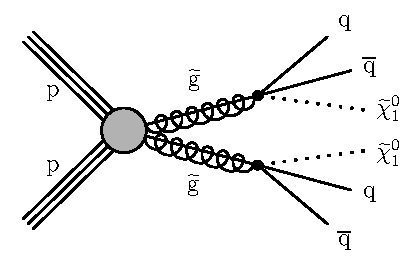
\includegraphics[width=0.3\textwidth]{figures/MT2_2019/Figure_007-a}
    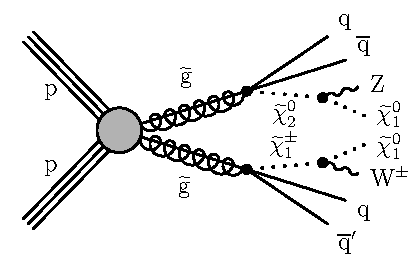
\includegraphics[width=0.3\textwidth]{figures/MT2_2019/Figure_007-b}
    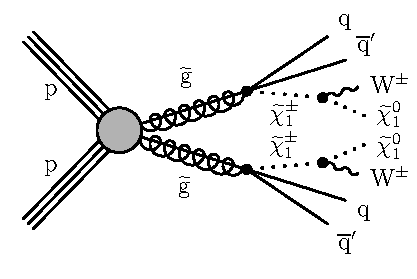
\includegraphics[width=0.3\textwidth]{figures/MT2_2019/Figure_007-c}\\
    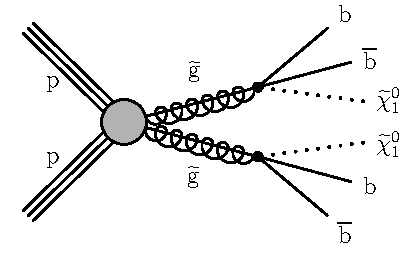
\includegraphics[width=0.3\textwidth]{figures/MT2_2019/Figure_007-d}
    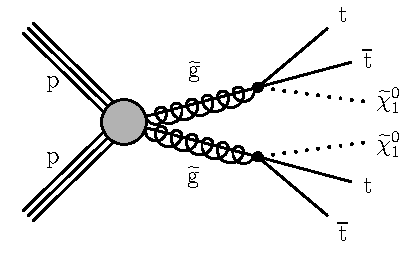
\includegraphics[width=0.3\textwidth]{figures/MT2_2019/Figure_007-e} \\
    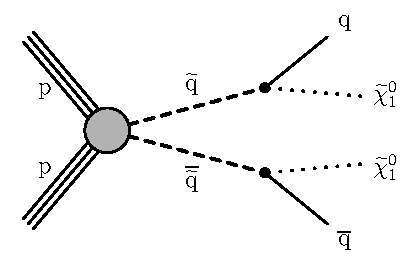
\includegraphics[width=0.3\textwidth]{figures/MT2_2019/Figure_007-f}
    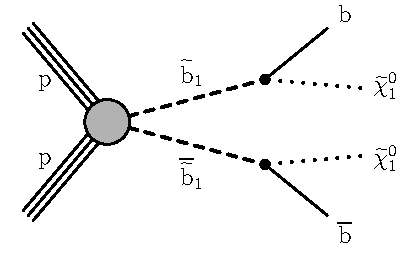
\includegraphics[width=0.3\textwidth]{figures/MT2_2019/Figure_007-g}
    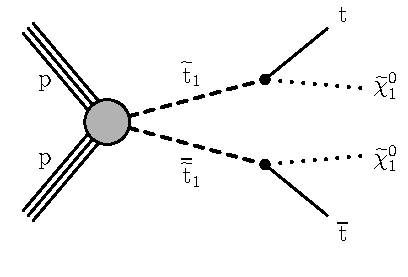
\includegraphics[width=0.3\textwidth]{figures/MT2_2019/Figure_007-h} \\
    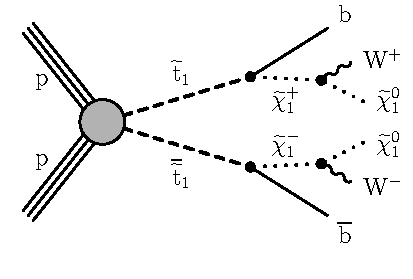
\includegraphics[width=0.3\textwidth]{figures/MT2_2019/Figure_007-i}
    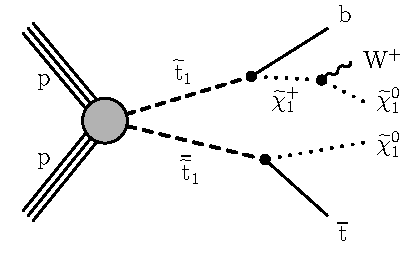
\includegraphics[width=0.3\textwidth]{figures/MT2_2019/Figure_007-j}
    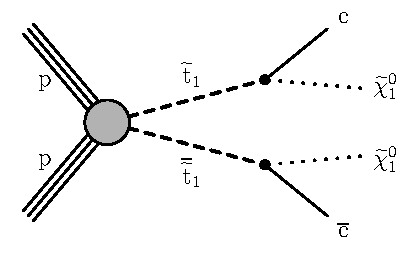
\includegraphics[width=0.3\textwidth]{figures/MT2_2019/Figure_007-k} \\
    \caption[Diagrams for gluino and squark pair production, as predicted by supersymmetric extensions of the Standard Model.]{Diagrams of gluino (upper five) and squark (lower six) pair production, as predicted by supersymmetric extensions of the Standard Model. 
The classic search considers five potential gluino decay chains. 
At upper left, the gluinos decay to light flavor quarks (up, down, strange, or charm), and the lightest neutralino, \lsp.
At upper center, the gluinos decay to light flavor quarks, but rather than decaying directly to \lsp, the gluinos decay either to the second neutralino, \chitwo, which subsequently decays to a Z boson and \lsp, or to the lightest chargino, \chargino, which subsequently decays to the W boson and \lsp, with equal probability.
At upper right, both gluinos undergo the \chargino to W decay chain.
On the left of the second row, both gluinos decay to bottom quark pairs and \lsp.
On the right of the second row, both gluinos decay to top quark pairs and \lsp.
Additionally, the classic search considers six potential modes of squark production and decay.
On the left of the third row, light flavor squarks decay to light flavor quarks and \lsp.
In the center of the third row, bottom squarks decay to bottom quarks and \lsp.
On the right of the third row, top squarks decay to top quarks and \lsp.
At lower left, top quarks decay to bottom squarks and \chargino, which subsequently decay to the W boson and \lsp.
At lower center, top squarks may undergo either the \chargino decay chain, or a direct decay to a bottom squark and \lsp, with equal probability.
At lower right, each top squark decays to a charm squark and \lsp.
Taken from \cite{MT2_2019}.}
    \label{fig:susyproduction}
  \end{figure}  

    The classic search generically targets any new physics that produces high \Ht events with jets and missing energy from undetected particles.
    Diagrams for several candidate models are shown in Figures~\ref{fig:susyproduction}, \ref{fig:monophidiag}, and \ref{fig:LQdiags}.
    The diagrams in Figure~\ref{fig:susyproduction} of gluino and squark pair production as predicted by supersymmetric extensions of the Standard Model are of greatest interest, and while the analysis is sensitive to a wide variety of similar hypothetical models, it is optimized for these.
    As discussed in Section \ref{sec:SUSYsms}, these models simplify the enormous parameter space of supersymmetric extensions by assuming that all superpartners except those in the process are so massive that they can be neglected entirely.
    The upper five diagrams all depict pair production of gluinos, the supersymmetric partner of the gluon, the mediating gauge boson of the strong interaction.
    As each gluino decays to two quarks, each of which will typically produce a jet, gluino pair production events tend to have many jets.
    Many different decay chains are possible, and the analysis considers five representative benchmarks.

    In the first benchmark, the gluinos decay to light flavor quarks (up, down, strange, or charm), and the lightest neutralino, \lsp.

    In the second benchmark, the gluinos decay to light flavor quarks, but rather than decaying directly to \lsp, the gluinos can decay either to the second neutralino, \chitwo, which subsequently decays to a Z boson and \lsp, or to the lightest chargino, \chargino, which subsequently decays to the W boson and \lsp.
    Each of these decays can occur with equal probability.
    Both the W and Z will themselves decay, usually to of pair of quarks, which will in turn produce jets. 
    So, relative to the first signal model, the second tends to have greater jet multiplicity.
    The Z can also decay to neutrinos, and the W can decay to a neutrino and a lepton that is not reconstructed.
    In these scenarios, this benchmark trades some jets for an enhanced missing energy signature.
    If  the W or Z decays leptonically and a lepton is successfully reconstructed, events from these signals may fail the lepton veto and instead end up in control regions, biasing the background prediction.
    The procedure used to handle such signal contamination of control regions is described in Section \ref{sec:MT2sigcontam}.

    The third benchmark, in which both gluinos undergo the \chargino to W decay chain, is similar.

    In the fourth benchmark, both gluinos decay to the bottom quark and \lsp.
    As described in Section \ref{sec:btagging}, it is possible to identify jets that originated from a bottom quark; such a jet is said to be ``b-tagged.''
    The classic search bins in the number of b-tagged jets in order to enhance sensitivity to signals of this type.

    In the fifth and final gluino pair-production benchmark, both gluinos decay to top quarks and \lsp.
    The top quark decays with probability near unity to a bottom quark and a W boson.
    The extra W bosons, compared to the direct bottom decay model, can either add jets or leptons and neutrinos, as previously discussed.
    This signal tends to produce the most remarkable events of any signal model considered, with very large \Ht, \njet, and \nb, but also loses many events to the lepton veto as any of the four W bosons is liable to produce a lepton.

    The lower six diagrams of Figure~\ref{fig:susyproduction} all depict pair production of squarks, the supersymmetric partners of quarks.
    Squark decays directly produce only one quark each, compared to two for gluino decays, so squark pair-production events tend to have fewer jets than gluino pair-production events.

    In the first squark benchmark diagram, on the left of the third row, a pair of light flavor squarks (up, down, strange, or charm) is produced and each decays to a light flavor squark and \lsp.
   
    In the second benchmark, bottom squarks are produced and decay to bottom quarks and \lsp.
    These events tend to have b-tagged jets, but fewer than in gluino decays to bottom squarks.

    In the third benchmark, top squarks are pair produced and decay to top quarks and \lsp.
    The relationship between this process and the previous one is similar to the relationship between the fifth and fourth gluino benchmarks, respectively.

    The fourth benchmark is very similar to the third.
    Instead of the top squark decaying directly to a top quark, which then decays to a bottom quark and W boson, the squark decays to a bottom quark directly and \chargino, which subsequently produces the W.
    While the final state particles are identical, their kinematics can be very different depending on the distribution of masses realized in nature.
    For instance, if the top squark and \chargino mass splitting is very small, the bottom quark jet in this benchmark may have such low \pt in a typical event that it is difficult to reconstruct.

    In the fifth benchmark, each top squark may undergo the \chargino decay chain or decay directly to a bottom squark and \lsp, with equal probability, mixing the two previous models.

    In the last benchmark, each top squark decays to a charm quark and \lsp.
    This decay chain could dominate when the top squark and \lsp mass splitting is too small to allow decay to on-shell top quarks, and the mass of \chargino is larger than that of the top squark.

    In each of these models, the mass of the squark or gluino and the mass of \lsp are free parameters.
    Large squark and gluino masses cause low production rates, as the production cross sections drop rapidly with increasing mass, as dicussed in Section \ref{sec:SUSYsms} and shown in Figure~\ref{fig:SUSYxsec}.
    The mass of \lsp does not affect the production rate, except insofar as it must be lower than the masses of all other superpartners, but it does affect the character of the events.
    When the mass splitting between the gluino or squark and \lsp is small, only a small portion of the event's energy ends up in the visible decay products, and most is lost to the rest energy of \lsp.
    These events have low \Ht and \met, low \njet, and when applicable, low \nb, and more closely resemble background.
    As the mass splitting increases, more energy shifts to the visible portion of the event, making events less background-like and increasing sensitivity.
    The analysis considers a grid of potential mass points for each model, and this sensitivity pattern is evident in the curves shown in Section \ref{sec:MT2limits}.
    
    The classic search also considers non-supersymmetric models.

    The first is referred to as the mono-$\phi$ model.
    In this model, a colored scalar boson much like a squark is produced singly, rather than pair-produced as in squark models in order to conserve R-parity, and decays to a quark and invisible fermion, as shown in Figure~\ref{fig:monophidiag}.
    This model has an especially low number of jets and low \mttwo, and so would appear in more background-like bins than most supersymmetric models.
    In fact, it was originally proposed \cite{monophi} to explain a potential excess in bins of this sort in the previous edition of the classic search, published based on 2016 data \cite{MT2_2016}, and so there is some interest in whether such an excess persists in the larger dataset.
    While the analysis is not optimized for models of this sort, indeed \mttwo is designed to target pair-production, it still has some residual sensitivity to any model characterized by jets and missing energy in the final state, including mono-$\phi$.

    The second non-supersymmetric model, and final model considered explicitly by the classic search, is leptoquark extensions of the Standard Model.
    As discussed in Section \ref{sec:othermodels}, while squarks can decay to a quark and \lsp, leptoquarks decay to a quark and a neutrino, which is experimentally effectively indistinguishable from a low mass \lsp.
    This last fact was first established in a reinterpretation of the 2016 edition of the classic search \cite{LQ2016}.
    Thus, it is a relatively simple exercise to reinterpret squark squark results in the low mass \lsp limit to leptoquark results.
    A few leptoquark production diagrams are shown in Figure~\ref{fig:LQdiags}.

  \begin{figure}[h!]
    \centering
    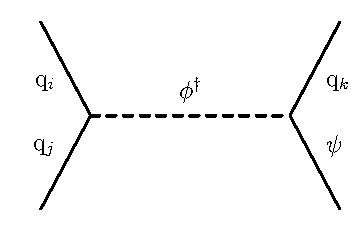
\includegraphics[width=0.85\textwidth]{figures/MT2_2019/Figure_008.pdf}
    \caption[Diagram for the mono-$\phi$ model.]{Diagram for the mono-$\phi$ model, in which a colored scalar $\phi$ is resonantly produced, and decays to an invisible massive Dirac fermion $\psi$ and an SM quark. Note that $\phi$ is not pair-produced, in contrast to otherwise-similar squarks. Taken from \cite{MT2_2019}.}
    \label{fig:monophidiag}
  \end{figure}  

  \begin{figure}[h!]
    \centering
    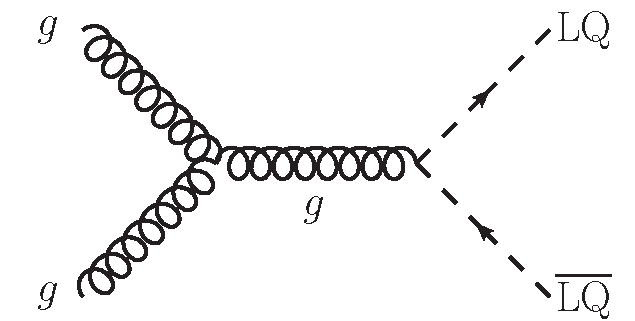
\includegraphics[width=0.3\textwidth]{figures/MT2_2019/Figure_009-a}
    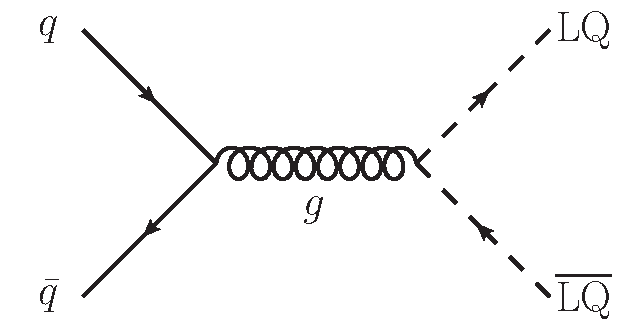
\includegraphics[width=0.3\textwidth]{figures/MT2_2019/Figure_009-b}\\
    \vspace{3mm}
    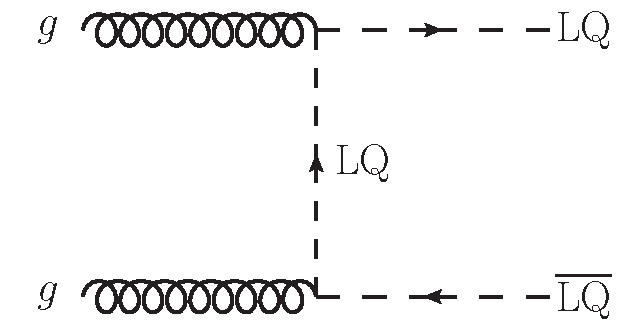
\includegraphics[width=0.3\textwidth]{figures/MT2_2019/Figure_009-c}
    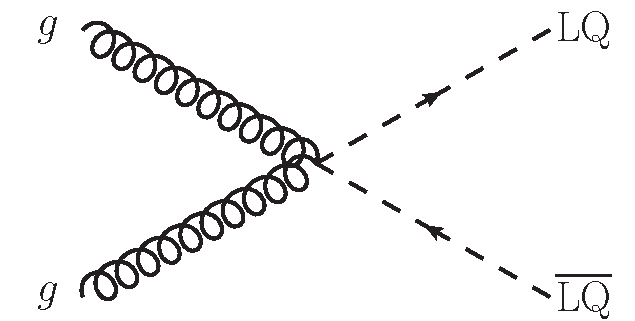
\includegraphics[width=0.3\textwidth]{figures/MT2_2019/Figure_009-d}
    \vspace{3mm}
    \caption[Leptoquark pair production diagrams.]{Diagrams of leptoquark pair production. Each lepqtoquark decays to a neutrino and a quark. Taken from \cite{MT2_2019}.}
    \label{fig:LQdiags}
  \end{figure}  

  \begin{table}[htb]
    \topcaption[Table of systematic uncertainties affecting expected signal yields.]{
      Systematic uncertainties in the signal yields for the simplified models of BSM physics.
      The large statistical uncertainties in the simulated signal sample come from a small number of bins with low acceptance,
      which are typically not among the most sensitive bins contributing to a given model benchmark point.
      Taken from \cite{MT2_2019}.
      \label{tab:sig_systs}}
    \centering
    \begin{tabular}{lc}
      \hline
      Source & Range [\%] \\
      \hline
      Integrated luminosity                     & 2.3--2.5     \\
      Limited size of MC samples                & 1--100  \\
      $b$-tagging efficiency, heavy flavors       & 0--40   \\
      $b$-tagging efficiency, light flavors       & 0--20   \\
      Lepton efficiency                         & 0--20   \\
      Jet energy scale                          & 5       \\
      Fast simulation \met modeling            & 0--5     \\
      ISR modeling                              & 0--30   \\
      $\mu_{\mathrm{R}}$ and $\mu_{\mathrm{F}}$  & 5       \\
      \hline
    \end{tabular}
  \end{table}
  By necessity and unlike backgrounds, the expected event yields for signal models are obtained directly from simulation.
  For this reason, while most uncertainties are shared with background, signal estimates are exposed to a few extra uncertainties, and some of the shared uncertainties increase in magnitude.

  First, while background is normalized to control region counts and so automatically scaled to the correct integrated luminosity, signal counts must be scaled by an independent measurement of the integrated luminosity.
  This measurement is only precise to within a few per cent, leading to a few per cent uncertainty on the expected event count.

  Second, additional jets obtained from ISR must be modeled in simulation for signal, while for background, the control regions provide a precise measurement of the relevant ISR jet production.
  In bins with many jets, where ISR jet production rates are less well-known and simultaneously more important, this uncertainty is as large as 30\%.

  Finally, signal models must be simulated in the fast-simulation framework discussed in Section~\ref{sec:limitations} to make the enormous array of signal scenarios considered computationally feasible.
  A systematic is assessed to cover potential errors made by this approximation.

  The remaining uncertainties are described in the next section, in the context of background estimates.

  \subsection{Backgrounds} \label{sec:MT2bg}

  All of the targeted signals are characterized by all-hadronic events with large missing energy, but observing such an event does not constitute discovery due to the existence of backgrounds that can produce the same basic signature.
  These backgrounds can be broadly divided into the detector mismeasurement background, in which apparent missing energy is generated not by genuine undetected particles but by an error in reconstruction, and the neutrino background, in which the missing energy is produced by genuine neutrinos as predicted in the Standard Model.
  The neutrino background can be subdivided into neutrinos originating from $W^{\pm}\rightarrow \ell^{\pm}\nu$, in which the presence of a charged lepton allows the neutrino to be rejected with good efficiency, and those originating from $Z\rightarrow \nu\nu$, in which the final state is entirely invisible and cannot be efficiently vetoed.

  
    \subsubsection{Mismeasurement} \label{sec:MT2QCD}
  
    The most problematic background is that caused by detector mismeasurement.
    Nearly every mismeasured event is a QCD multijet event, because nearly every event at a proton-proton collider is a QCD multijet event and the probability of mismeasurement is roughly flat across events. 
    Accordingly, the mismeasurement background is also referred to as the QCD multijet background.
    While the detector makes mistakes only very rarely, QCD events are so relatively common that this background is still dominant in the raw dataset, before any cleaning selections.

    Estimating the QCD background is challenging because it requires highly detailed knowledge of the detector's idiosyncrasies.
    Rather than risk falsely discovering a signal or failing to identify one that is present due to misprediction of this background, the analysis adopts selections designed to suppress it, until the background is sufficiently minor that large relative error in its prediction is acceptable.
    
    The first and most powerful of these selections uses the \mttwo variable described in Section \ref{sec:MT2}, namely $\mttwo > 200$~GeV, where the value is chosen to achieve the desired suppression of the mismeasurement background.
    Although the \mttwo selection is somewhat expensive in the sense that it eliminates a significant fraction of signal, especially for signals with a small mass splitting and signals like mono-$\phi$ that are not pair-produced, it is crucial for suppressing the mismeasurement background.
    At $\Ht > 1500$~GeV, the mismeasurement background extends unacceptably beyond $\mttwo \sim 200$~GeV, and the \mttwo selection is tightened to $\mttwo > 400$~GeV.

    The second selection uses the observable 
    $$\dphimin = \textrm{Min}\left(\left|\phi_{\met}-\phi_i\right|\right)$$
    where $\phi_i$ indicates the $\phi$ coordinate of the $i$th \pt jet and $\phi_{\met}$ is the $\phi$ coordinate of the missing energy vector.
    Stated simply, \dphimin is the smallest angular separation in the transverse plane of the missing energy vector and any of the four highest \pt jets.
    Close overlap between a jet and the missing energy vector indicates a high probability that the jet was badly mismeasured, and is itself the source of the \met in the event.
    The selection applied is $\dphimin > 0.3$, where the value is chosen to achieve strong background rejection without too great a loss of signal efficiency.
    Only the four highest energy jets are used because the probability of {\it some} jet overlapping the missing energy vector approaches unity as the number of jets increases, so the selection would nearly always veto high \njet\xspace events, and the high \njet\xspace bins are sufficiently signal-rich that aggressive background rejection is not as necessary.
    The effect of this selection is depicted in Figure~\ref{fig:dphimin}, after an \mttwo selection of only 100 GeV.

    The last selection rejects events in which a suspiciously large fraction of the missing energy comes from very soft objects.
    The minimum \pt for selected jets is 30~GeV.
    The missing energy vector from only jets is denoted $\vec{\HTm}$.
    The missing energy vector used in the analysis, $\vec{\met}$, uses all PF candidates, including those outside jets or in jets with $\pt < 30$~GeV.
    If these two quantities are very different, it means that a large portion of the \met in the event was generated by these low \pt objects, a sign that something may have gone wrong in reconstruction.
    Specifically, the selection is $\left|\vec{\HTm}-\vec{\met}\right|/\met < 0.5$.

    \begin{figure}[h!]
      \centering
      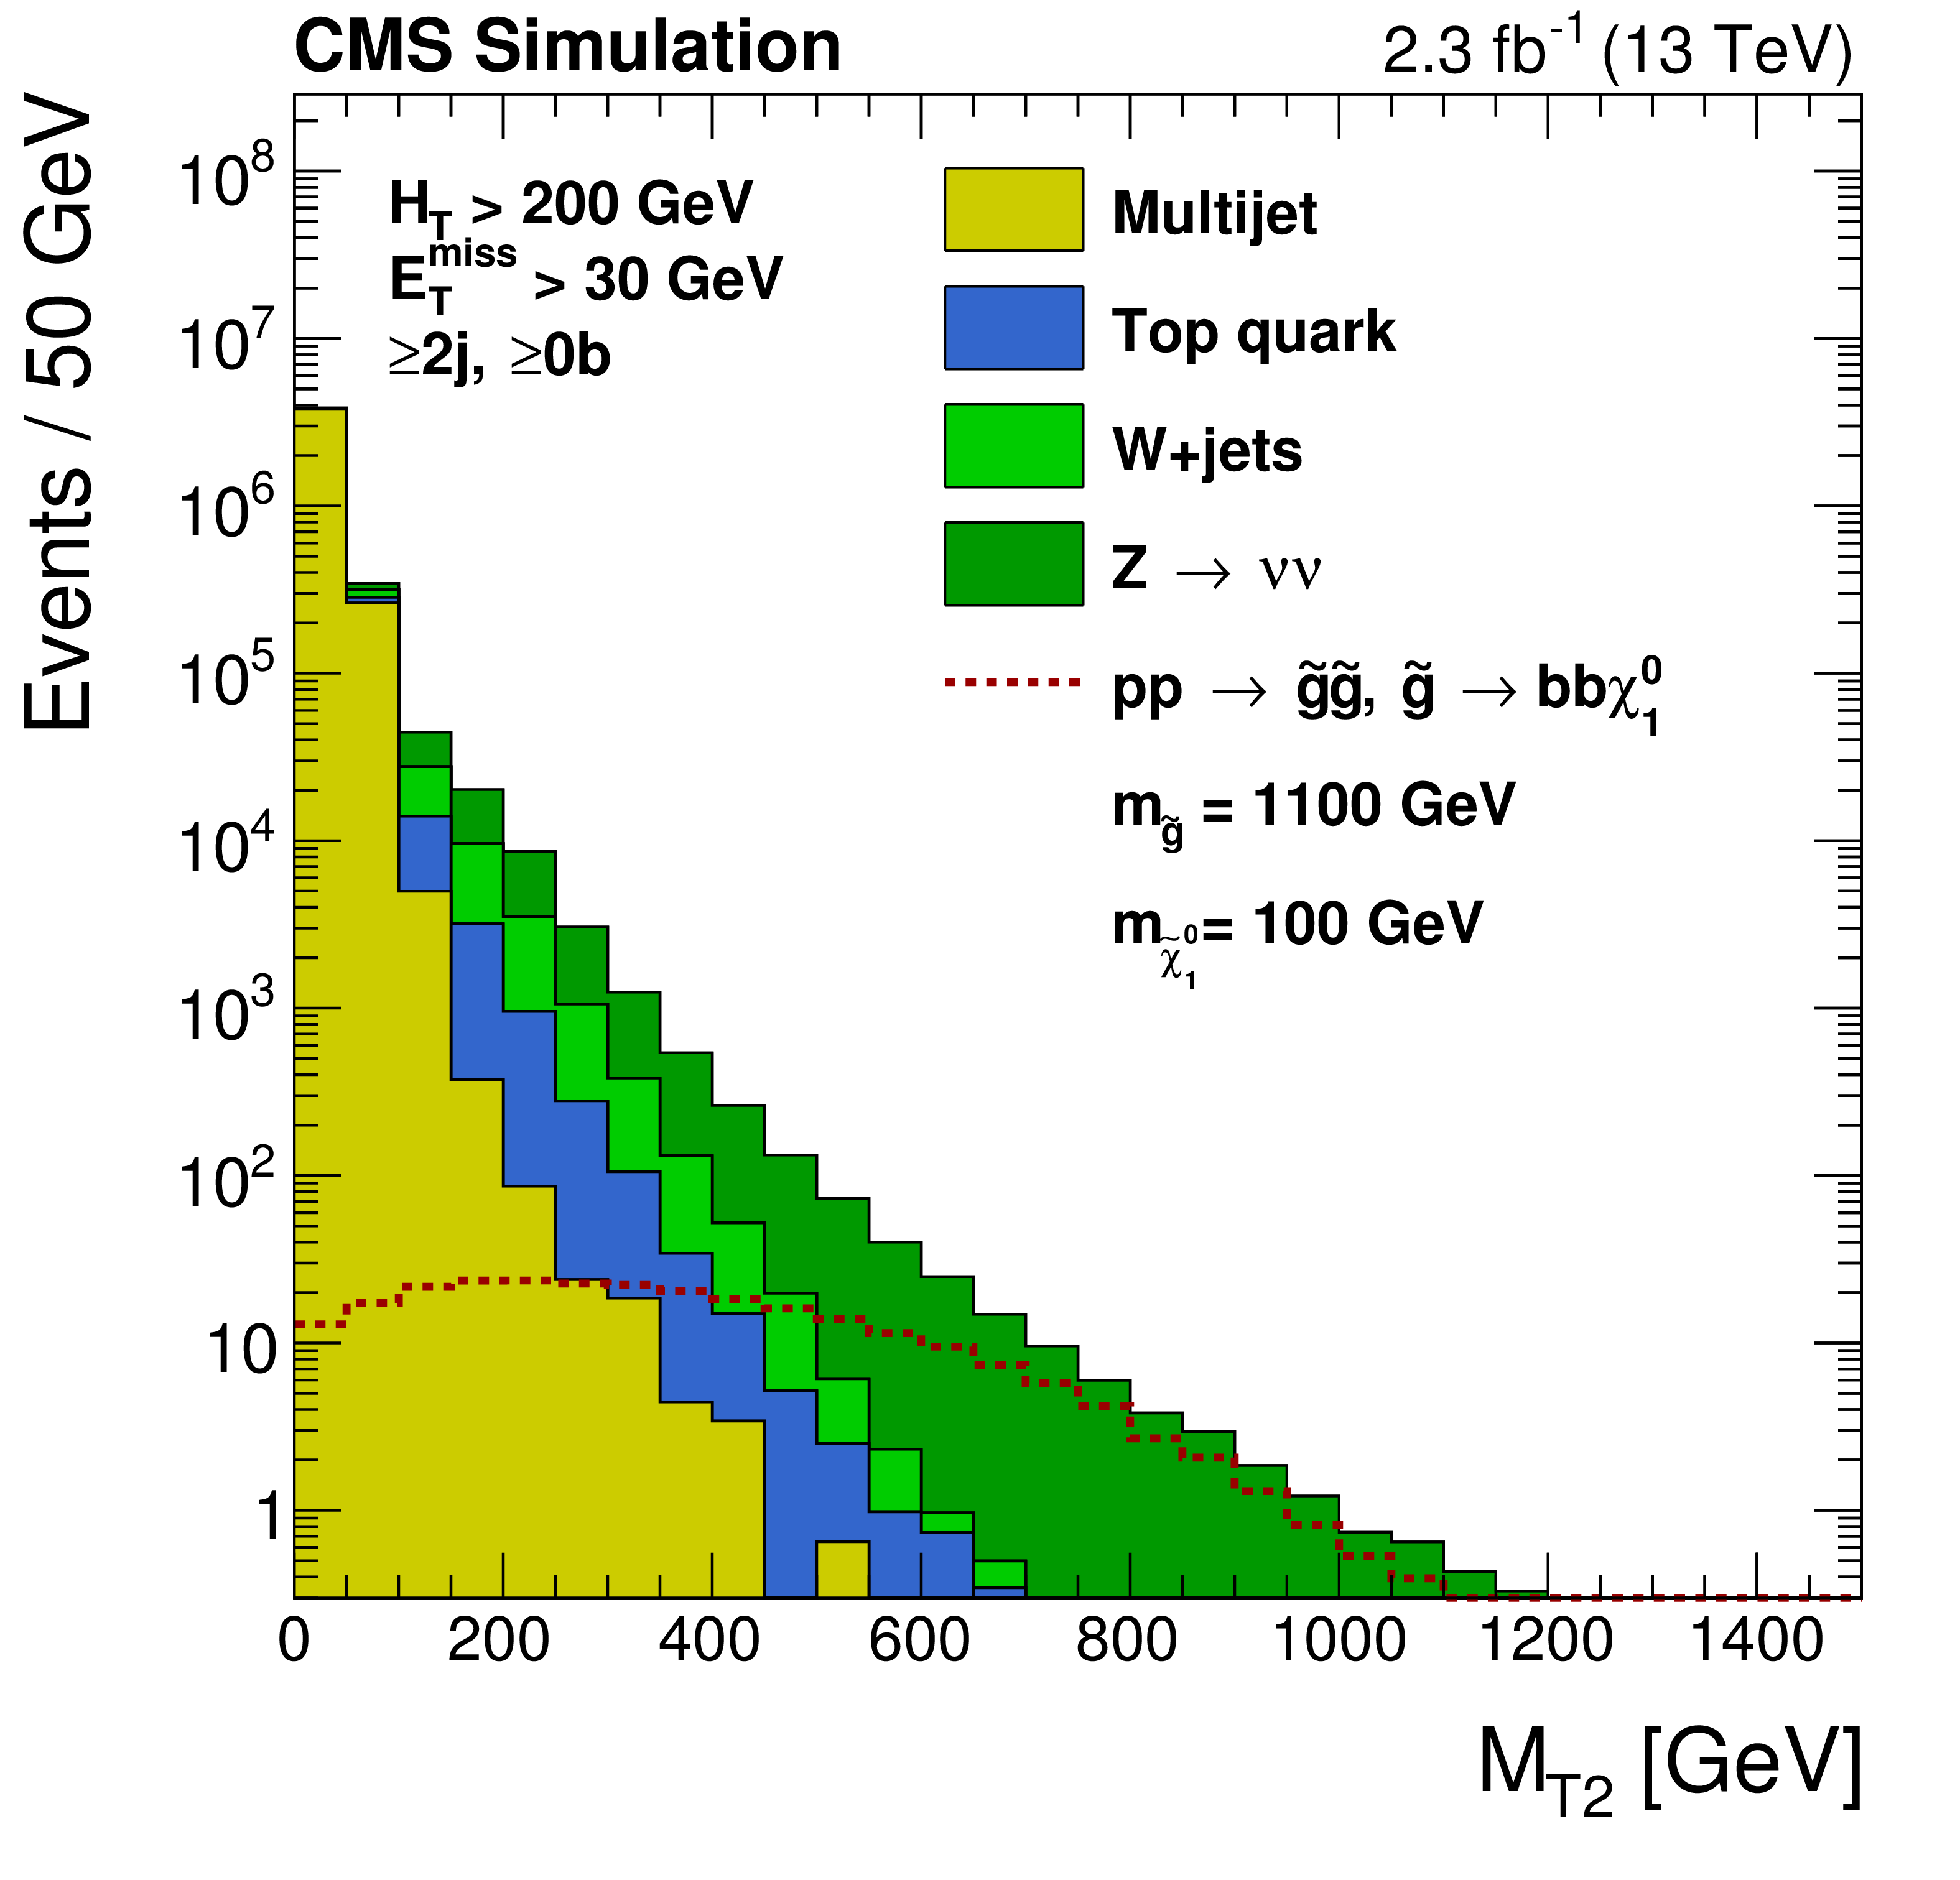
\includegraphics[width=0.48\textwidth]{figures/mt2_mt2_2015.png}
      \caption[\mttwo distributions of backgrounds and an example signal point.]{The distributions in \mttwo of the QCD background (filled yellow) and the neutrino backgrounds (filled blue and green) are stacked and overlaid with an example signal point (gluino pair production and decay to bottom quarks, in red). Even with other mismeasurement-suppression selections applied, the mismeasurement background still dominates without $\mttwo > 200$~GeV. Taken from \cite{MT2_2015}.}
      \label{fig:mt2dist}
    \end{figure}  
    
    \begin{figure}[h!]
      \centering
      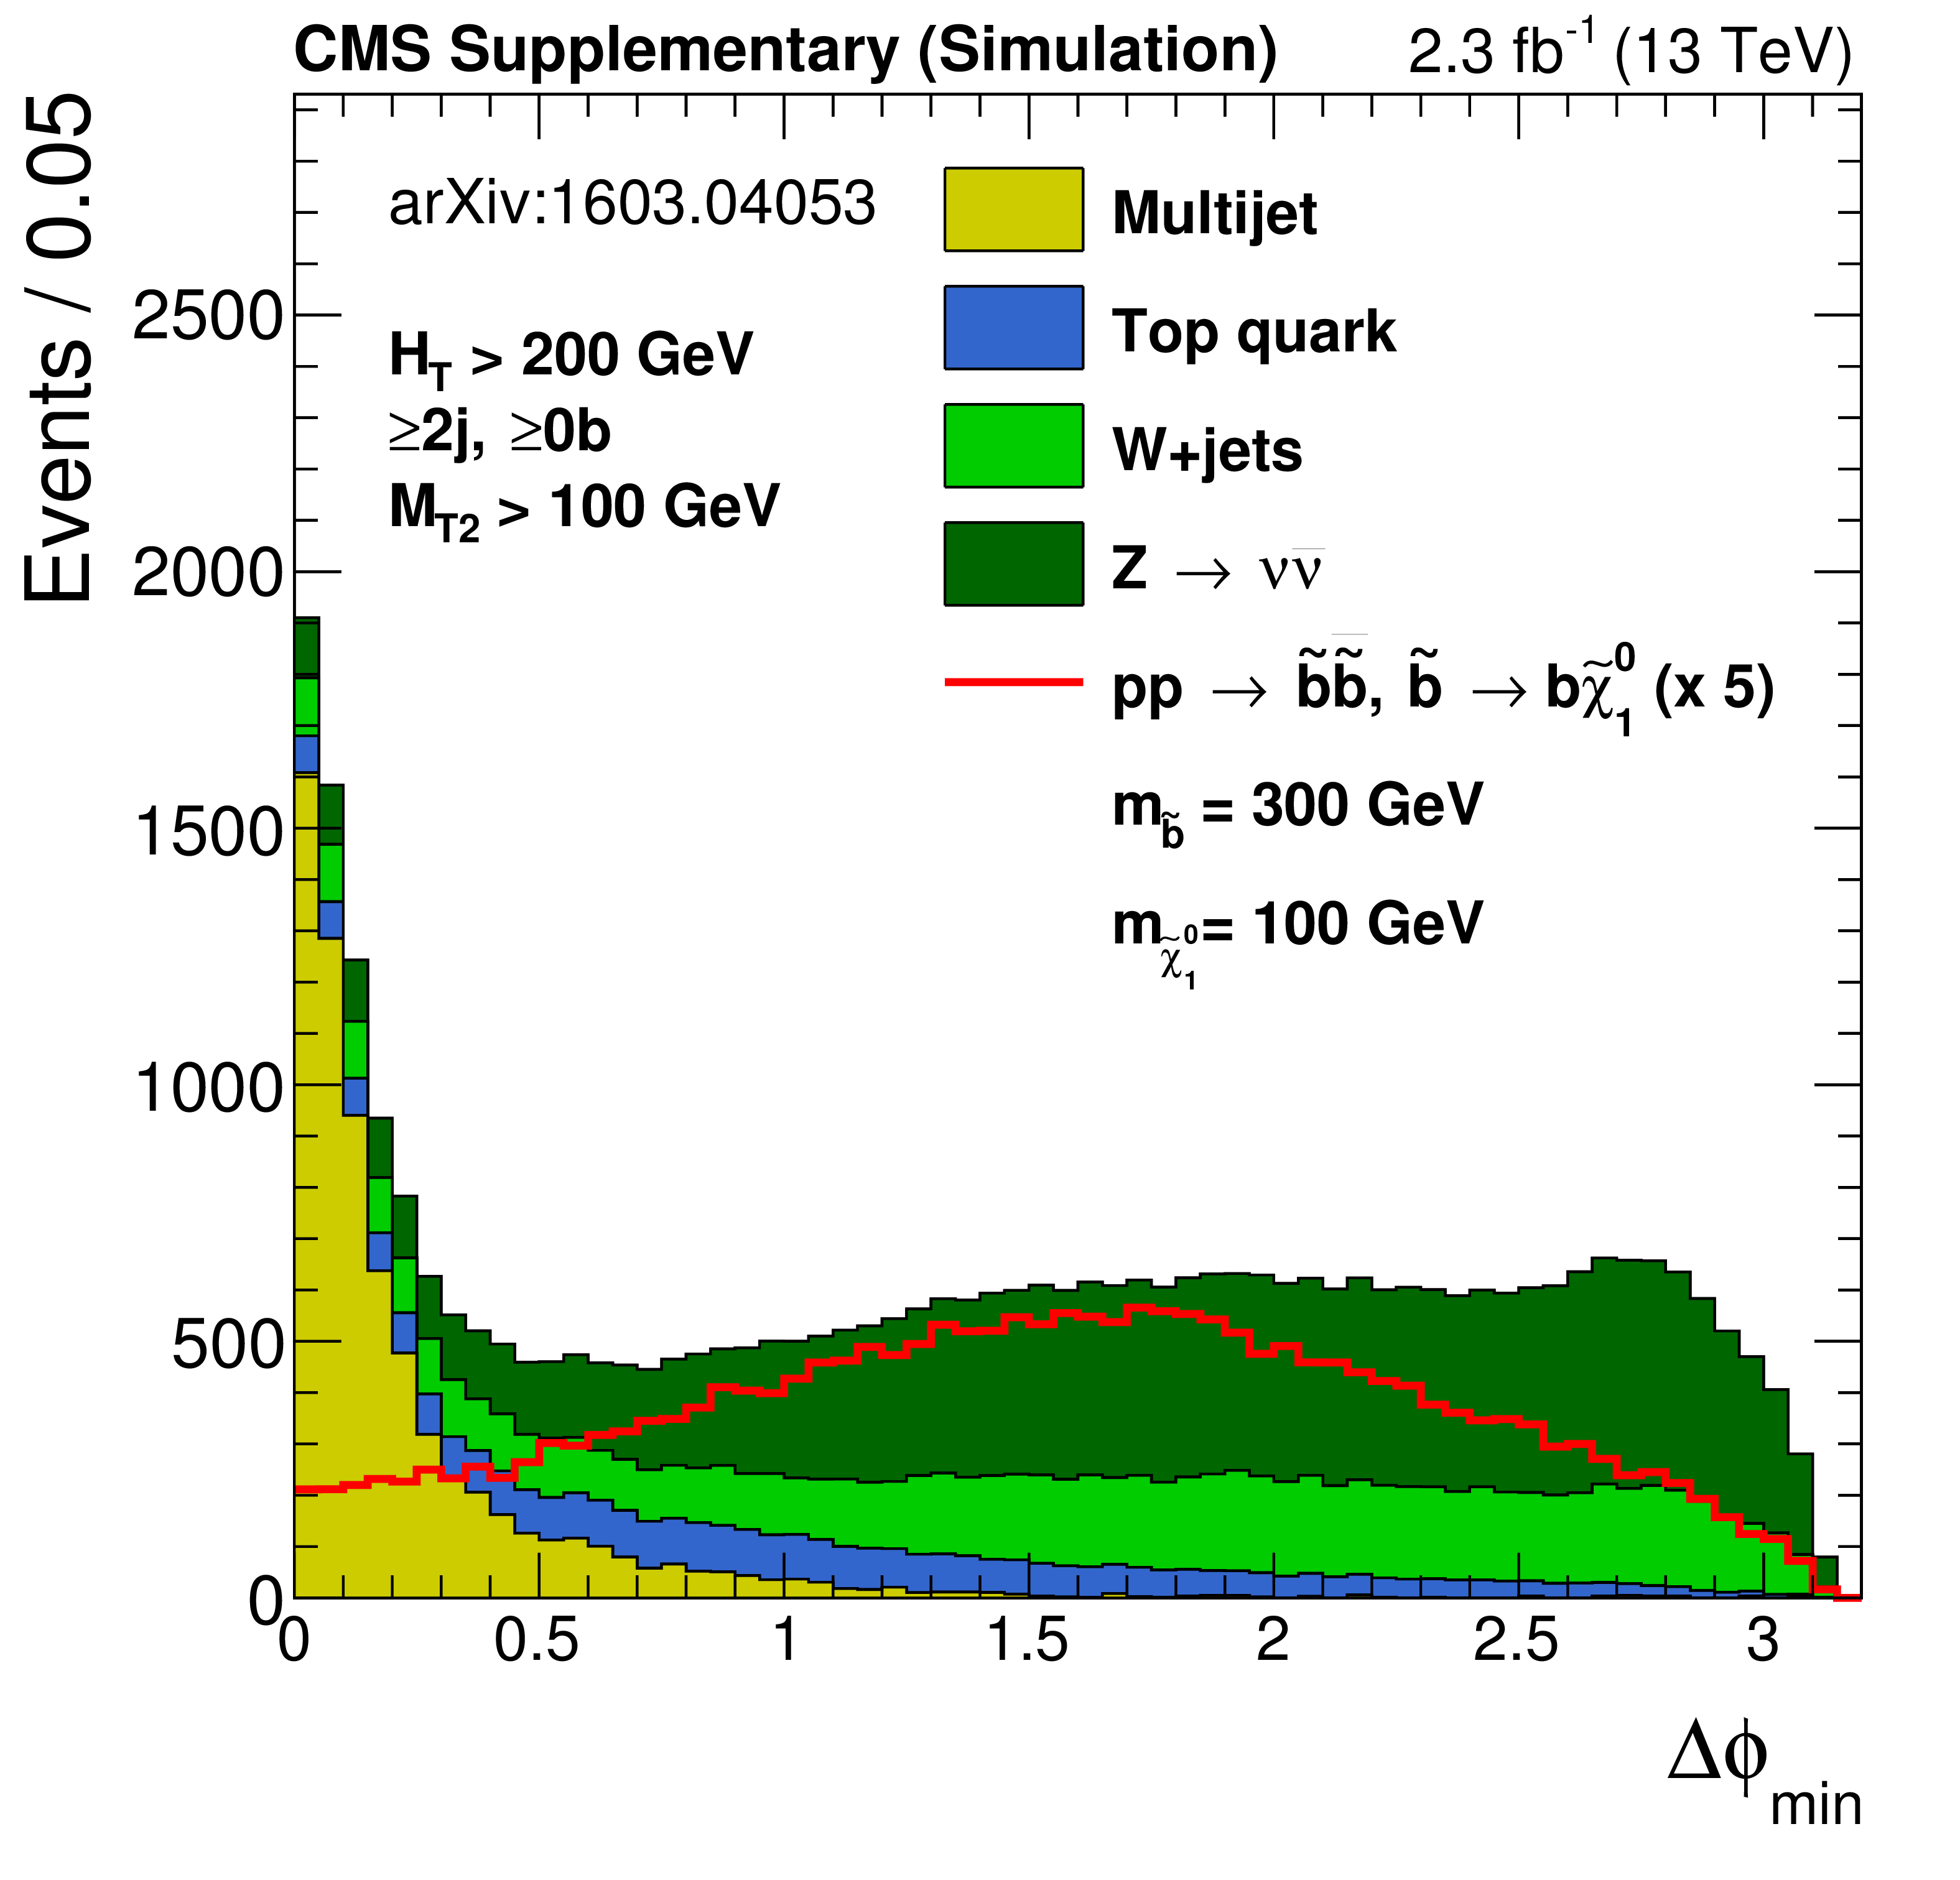
\includegraphics[width=0.48\textwidth]{figures/mt2_dphi_2015.png}
      \caption[\dphimin distributions of backgrounds and an example signal point.]{The distributions in \dphimin of the QCD background (filled yellow) and the neutrino backgrounds (filled blue and green) are stacked and overlaid with an example signal point scaled up by a factor of 5 (bottom squark pair production, in red), with the \mttwo selection relaxed to 100 GeV. Note that most QCD lies below the cut value of 0.3. Taken from \cite{MT2_2015} supplementary materials.}
      \label{fig:dphimin}
    \end{figure}  
    
    The residual mismeasurement background is estimated using a procedure called Rebalance and Smear that was newly implemented for this edition of the classic analysis, and described in Section \ref{sec:RandS}.
    
    \subsubsection{Lost Lepton} \label{sec:MT2lostlep}

    The lepton veto rejects most events containing neutrinos originating from the decay of a W boson, $W^{\pm}\rightarrow \ell^{\pm}\nu$.
    However, the lepton is not always successfully reconstructed, usually because the lepton is a $\tau$ that decays hadronically and is mistaken for a meson, and this residual so-called lost lepton background must be estimated. 

    A first attempt might be to simulate events containing W bosons, scale the simulation to the desired luminosity, and count the events in which the lepton is not reconstructed.
    This procedure would have reasonable accuracy, but producing accurate simulations is not trival, and the result would be subject to an array of systematic errors.
    Schematically, if $N_{LL}^{\mathrm{Data}}$ is the actual number of lost lepton events in data and $N_{LL}^{\mathrm{MC}}$ is the number predicted by Monte Carlo simulation, the simulation will mispredict by some factor $\epsilon$ such that $N_{LL}^{\mathrm{Data}} = \epsilon N_{LL}^{\mathrm{MC}}$.

    It is possible to do better than $\epsilon$ with data driven techniques.
    In addition to the lost lepton events, one can also ask the simulation for its prediction of the number of W events in which the lepton is not lost, single lepton events, $N_{SL}^{\mathrm{MC}}$, where we restrict the lepton to electrons and muons since $\tau$ reconstruction is much more difficult.
    Every part of this simulation is exactly identical to the lost lepton simulation, subject to almost the same errors, with the major exception being the predicted lepton reconstruction efficiency.
    Call this new error factor $\delta$ so that $N_{SL}^{\mathrm{Data}}=\delta N_{SL}^{\mathrm{MC}}$.
    Then $\epsilon/\delta = \gamma$ is the portion of the misprediction due to the simulation's imperfect knowledge of the lepton reconstruction efficiency and a few other more minor uncorrelated effects, a small portion of the total.
    The ratio $R_{\mathrm{MC}}^{0\ell/1\ell} = N_{LL}^{\mathrm{MC}} / N_{SL}^{\mathrm{MC}}$ is subject only to this relatively small error $\gamma$, since the fully correlated errors cancel.
    The prediction of $N_{LL}^{\mathrm{Data}}$ follows directly,
    \begin{equation}
      N_{LL}^{\mathrm{Data};Est} = R_{\mathrm{MC}}^{0\ell/1\ell} N_{SL}^{\mathrm{Data}}.
    \end{equation}
    The input $N_{SL}^{\mathrm{Data}}$ is measured in a control region populated by single lepton events observed in data, in a kinematic region identical to the corresponding lost lepton signal region.
    The remaining systematic uncertainty is only about 15\% in most signal regions.

    \begin{table}[tbhp]
      \centering
      \topcaption[Table of uncertainties affecting the lost lepton background estimate.]{\label{tab:llepsyst}
        Summary of systematic uncertainties in the lost-lepton background prediction, together with their typical size ranges across the search bins. 
        ($\dagger$) In every topological region, bins along the \mttwo axis with insufficient statistics to allow a fully data-driven estimate are assigned an \mttwo shape from simulation, normalized based on the integral of the affected bins in the data control region.
        Taken from \cite{MT2_2019}.
      }
      \begin{tabular}{ l  c }
        \hline
        Source & Range [\%] \\
        \hline
        Limited size of data control samples & 5--100\\
        Limited size of MC samples & 0--50\\
        $e/\mu$ efficiency & 0--10\\
        $\tau$ efficiency & 0--3\\
        $b$-tagging efficiency & 0--3\\
        Jet energy scale & 0--5\\
        $\Mt\left(\text{lepton},~\vec{\met}\right)$ selection efficiency & 0--3\\
        \mttwo shape uncertainty$^{\dagger}$ & 0--40\\
        Renormalization and factorization scale variation & 0--5\\
        $t\bar{t}b\bar{b}/t\bar{t}jj$ weight & 0--25\\
        \hline
      \end{tabular}
    \end{table}
    Other uncertainties affecting the lost lepton background prediction are summarized in Table~\ref{tab:llepsyst}, together with their typical size ranges across the search bins.
    The first two uncertainties due to limited data control region and Monte Carlo simulation sample sizes are purely statistical.
    The remainder are systematic.

    The efficiency to reconstruct leptons is, as mentioned, the primary uncertainty of the simulation with respect to data, that does not drop out after taking a ratio of lost- and single-lepton events.

    The impact of the $\tau$ reconstruction efficiency is smaller, as it is not used in the single lepton control region, however uncertainty on the rate at which the $\tau$ veto fails to reject events contributes to uncertainty in the expected yield.

    The expected transfer factor from the single lepton to lost lepton regions varies slightly with respect to the binning variables, \Ht, \njet, \nb, and \mttwo, and so is recalculated in simulation for each bin.
    Since the transfer factor varies, they may be incorrectly estimated if simulation does not accurately reproduce the $b$-tagging efficiency and jet energy assignments in real data.

    To restrict the single lepton control region to leptons consistent with originating from a leptonic W decay, the lepton and \met system is required to satisfy $\Mt\left(\text{lepton},~\vec{\met}\right) < 100$~GeV, since an on-shell W can never decay to a lepton-neutrino system more massive than this, and $\Mt \leq M$.

    The renormalization and factorization scales are generic issues with theoretical calculations, discussed in Section~\ref{sec:limitations}.

    Finally, the $t\bar{t}b\bar{b}/t\bar{t}jj$ weight is a special systematic assessed to cover an ad hoc procedure that corrects a particularly severe data-simulation discrepancy affecting the relative rates of $b\bar{b}$ ISR and light flavor ISR in simulated $t\bar{t}$ events.
    This simulation error is not significant for the majority of CMS analyses, however it is important for analyses like this search that include bins with large \nb, for which $t\bar{t}b\bar{b}$ is the only meaningful background.

    In closing, it should be noted that while the lost lepton background tends to be subdominant relative to the Invisible Z background discussed in the next section, it is the largest background in certain high \njet, high \nb, high \Ht bins since Z events do not populate these bins efficiently, while $t\bar{t}$ pair-production events do, and all $t\bar{t}$ events contain two W bosons that may decay leptonically.

    \subsubsection{Invisible Z} \label{sec:MT2zinv}

    The $Z\rightarrow \nu\nu$ background is predicted in a similar fashion to the lost lepton background, using a control region populated with $Z\rightarrow \ell^+\ell^-$ events.
    Again, the leptons are restricted to pairs of electrons and pairs of muons, since $\tau$ reconstruction is much more difficult.    
    Figure~\ref{fig:Zestimate} (right) shows the similarity in the \mttwo distributions of simulated \znunu events and observed \zll events in which one pretends that the leptons are invisible, demonstrating both that these events are kinematically very similar as expected, and that the simulation is accurate.
    The ratio $R_{MC}^{\nu\nu/\ell^+\ell^-}$ can be extracted from Monte Carlo simulation, and is dominated by only the lepton reconstruction efficiency uncertainty.
    In the Standard Model, this ratio is almost exactly 3, but it is significantly larger experimentally because it is possible for one of the leptons in $Z\rightarrow\ell^+\ell^-$ not to be well-reconstructed, causing the affected event not to be counted.
    The value $N_{\ell^+\ell^-}^{Data}$, unlike $N_{SL}^{Data}$, is not trivial to extract, since a non-negligible fraction of double lepton events come from sources other than a single Z boson, 
    almost always one each from a pair of W bosons.
    $N_{\ell^+\ell^-}^{MC}$ and $N_{\nu\nu}^{Data}$ are exclusively $Z\rightarrow \ell^+\ell^-$ and $Z\rightarrow\nu\nu$ events, respectively, and for maximal cancellation of systematic uncertainties, it is desirable that $N_{\ell^+\ell^-}^{Data}$ be purified to the greatest extent possible.

  \begin{figure}[h!]
    \centering
    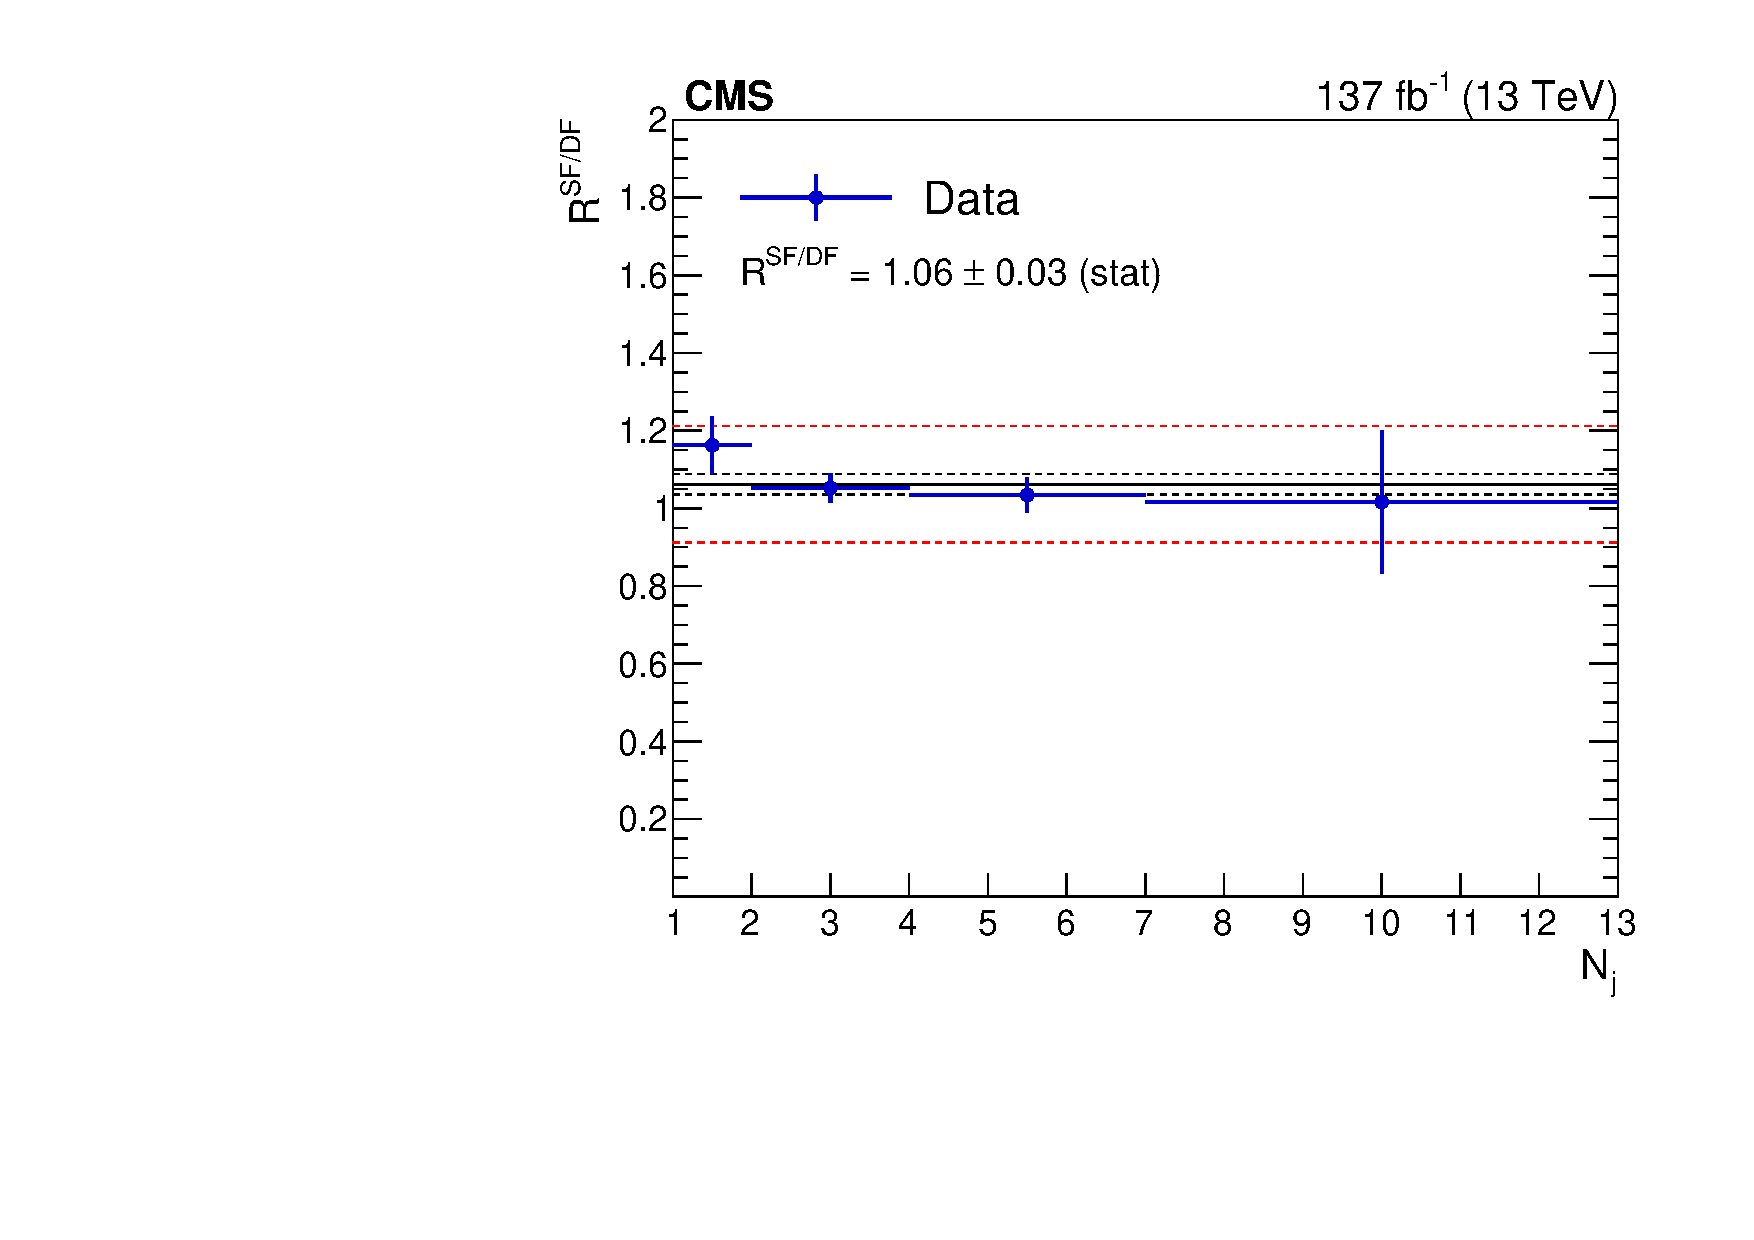
\includegraphics[width=0.53\textwidth]{figures/MT2_2019/Figure_002-a.pdf}
    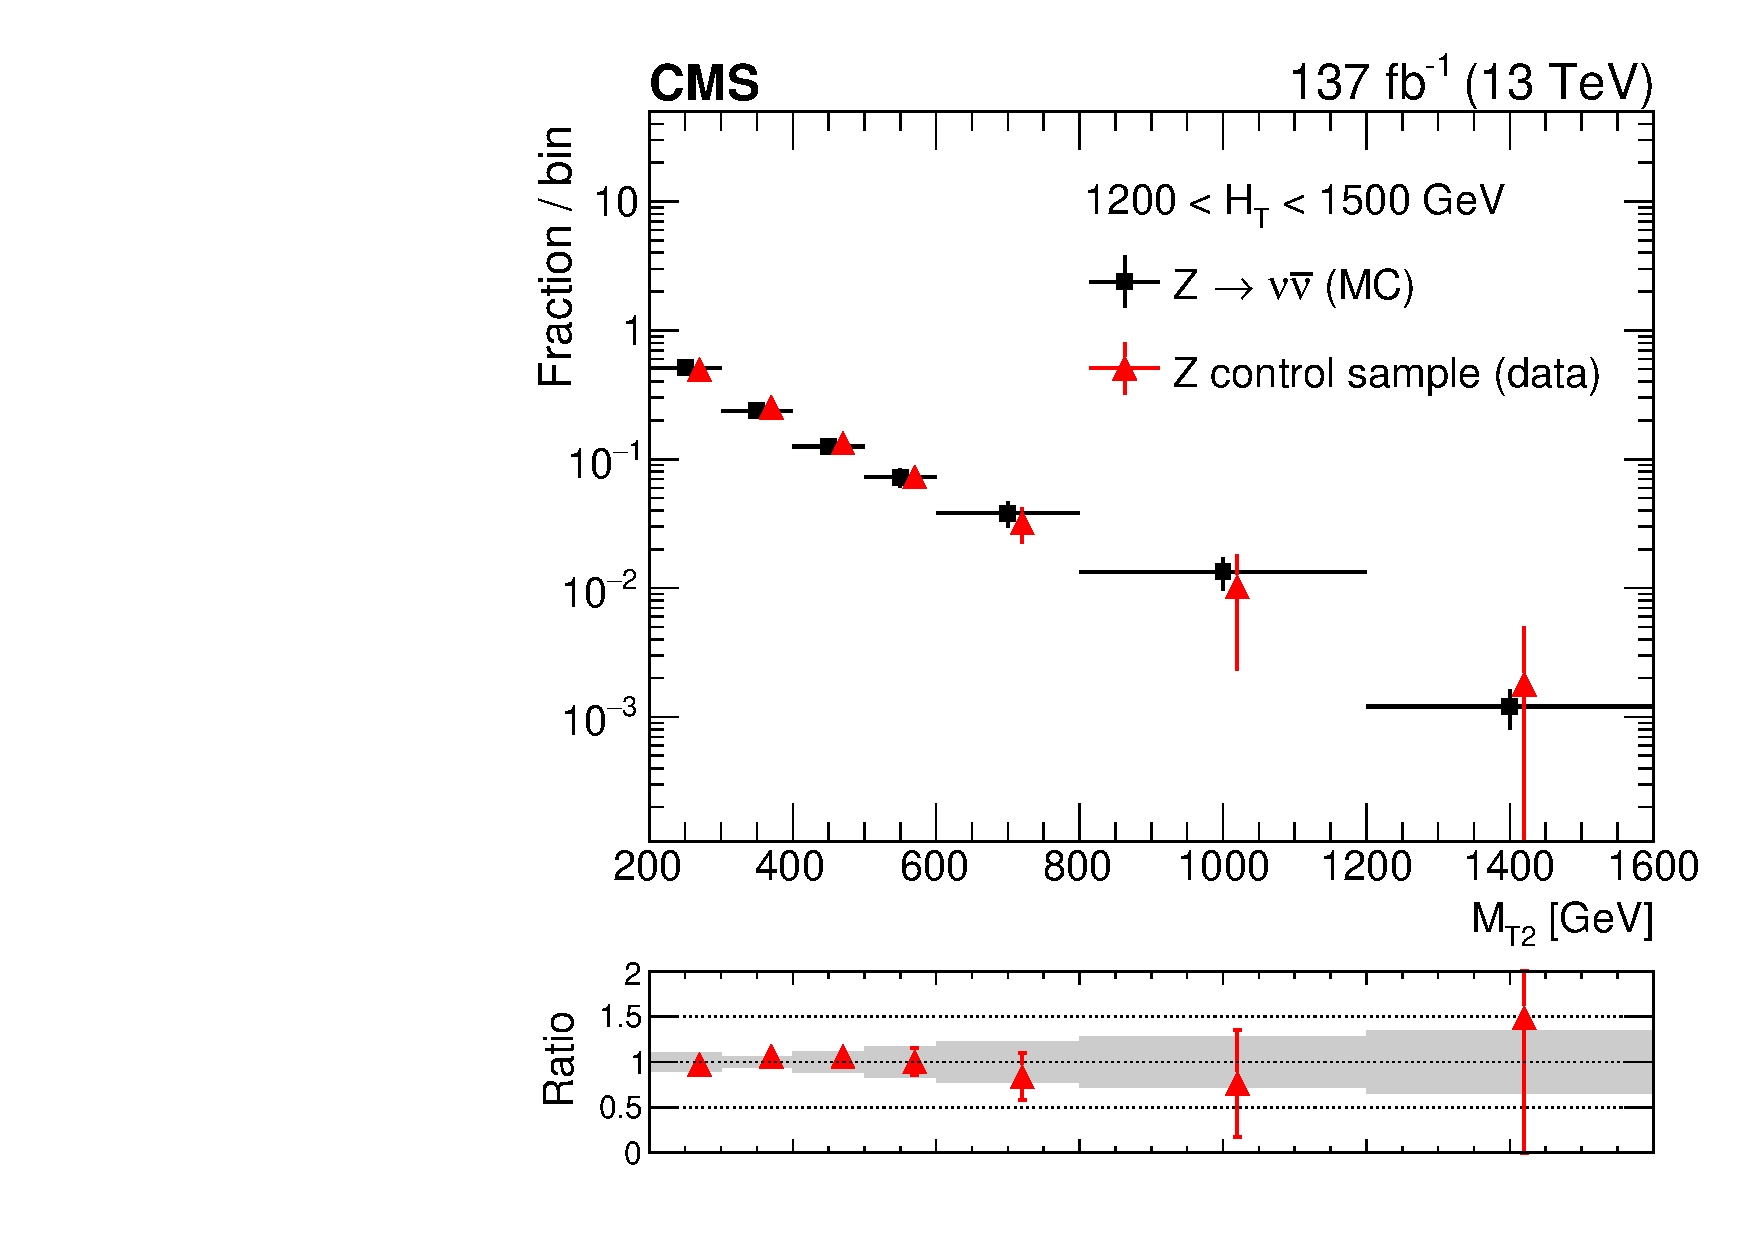
\includegraphics[width=0.44\textwidth]{figures/MT2_2019/Figure_002-b.pdf}
    \caption[(Left) The ratio of the number of same flavor to different flavor lepton pairs in data. (Right) A comparison of the \Mttwo shape between data Z to lepton events and simulated Z to neutrino events.]{
      (Left) The ratio of the number of same flavor to different flavor lepton pairs in data, $R^{SF/DF}$, which is a component of the $Z\rightarrow\nu\nu$ background estimate from $Z\rightarrow\ell^+\ell^-$ events. (Right) A comparison of the \Mttwo shape between data $Z\rightarrow\ell^+\ell^-$ events and simulated $Z\rightarrow\nu\nu$ events. The two processes should be kinematically identical, and the similarity of the distributions indicates that the Monte Carlo simulation models the processes well. Taken from \cite{MT2_2019}.}
    \label{fig:Zestimate}
  \end{figure}  

    Fortunately, there is an experimental handle on the contamination.
    When a Z boson decays to a lepton pair, the flavor is always identical, either two electrons or two muons.
    When a pair of W bosons each decay to a lepton pair, their choices are uncorrelated.
    Half the time, the flavors will be identical as for a Z event, and half the time, one W will decay to a muon and the other to an electron.
    The first case is the undesired impurity in $N_{\ell^+\ell^-}^{Data}$, and events of the second type are used to populated a different-flavor control region used to predict the impurity, $N_{DF}^{Data}$.
    It is nearly sufficent simply to subtract $N_{DF}^{Data}$ from $N_{\ell^+\ell^-}^{Data}$ since the different flavor and same flavor W events occur at the same rate.
    However, it is possible that the detector is slightly more or less efficient at reconstructing events where both leptons are the same flavor than events in which they are different flavors, so the different flavor count must be scaled slightly to compensate, by a factor $R^{SF/DF}$.
    $R^{SF/DF}$ is measured in data in $\ell^+\ell^-$ events that are kinematically inconsistent with originating from a Z decay, chiefly due to a requirement that the invariant mass of the lepton pair be at least 20~GeV away from the Z mass.
    One finds that $R^{SF/OF} \approx 1.06 \pm 0.15$, as shown in Figure~\ref{fig:Zestimate} (left).
    The final prediction is
    \begin{equation}
      N_{\nu\nu}^{Data;Est} = R_{MC}^{\nu\nu/\ell^+\ell^-}(N_{Data}^{\ell^+\ell^-}-R^{SF/OF}N_{DF}^{Data})
    \end{equation}
    Being irreducible, the \znunu plus jets background is dominant in the vast majority of bins.

    \begin{table}[tbhp]
      \centering
      \topcaption[Table summarizing the systematic uncertainties affecting the \znunu background prediction.]{\label{tab:invzsyst}
        Summary of systematic uncertainties in the \znunu background prediction,
        together with their typical size ranges across the search bins.
        ($\dagger$) In every topological region, bins along the \mttwo axis with insufficient statistics to allow a fully data-driven estimate are assigned an \mttwo shape from simulation, normalized based on the integral of the affected bins in the data control region.
        Take from \cite{MT2_2019}.
      }
      \begin{tabular}{ l  c }
        \hline
        Source & Range [\%] \\
        \hline
        Limited size of data control samples & 5--100\\
        Limited size of MC samples & 0--50\\
        Lepton efficiency & 0--5\\
        Jet energy scale & 0--5\\
        Uncertainty in $R^{\mathrm{SF}/\mathrm{DF}}$ & 0--5\\
        \mttwo shape uncertainty$^{\dagger}$ & 0--40\\
        \hline
      \end{tabular}
    \end{table}
    The uncertainties in the \znunu background prediction are summarized in Table~\ref{tab:invzsyst} together with their typical size ranges across the search bins.
    Only the uncertainty in $R^{\mathrm{SF}/\mathrm{DF}}$ is unique to \znunu, while the others are shared with the lost-lepton estimate.

  \subsection{Baseline Selection} \label{sec:MT2baseline}

  \begin{table}[htbp]
    \scriptsize
    \centering
    \renewcommand{\arraystretch}{1.3}
    \begin{tabular}{c c l}
      Observable               & Selection   & Notes \\
      \hline
      \mttwo                   & $> 200$~GeV & Only for multijet events. Increased to $\mttwo > 400$~GeV for $\Ht > 1500$~GeV to maintain QCD suppression. \\
      $\pt^{\mathrm{Jet 1}}$   & $> 250$~GeV & Only for monojet events. \\
      \Ht                      & $> 250$~GeV & Motivated by available triggers. Background events at lower \Ht are too common for these events to be always recorded. \\
      \met                     & $> 250$~GeV & Relaxed to $\met > 30$~GeV for $\Ht > 1200$~GeV. Motivated by available triggers. \\
      \dphimin                 & $> 0.3$     & Auxiliary mismeasurement suppression. \\
      $\left|\vec{\HTm} - \vec{\met}\right|/\met$ & $< 0.5$ & Auxiliary mismeasurement suppression. \\
      \nlep                    & $= 0$       & The lepton veto; rejects the majority of $W^{\pm}\rightarrow\ell^{\pm}\nu$ background. \\
    \end{tabular}
    \caption[Summary table of baseline event selection.]{A summary of the baseline event selection for the classic \mttwo search.
      Events are required to have large \Ht, no leptons, and significant missing energy unlikely to be the product of detector mismeasurement or a single undetected particle.}
    \label{tab:baseline}
  \end{table}

  The properties of these signals and backgrounds motivate the baseline event selection summarized in Table \ref{tab:baseline}.
  The \mttwo selection primarily suppresses the mismeasurement background, by many orders of magnitude.
  The \dphimin and \HTm selections also help to suppress this background further, until it is smaller than the genuine \met backgrounds.
  The \Ht and \met selections are chosen primarily so that all of the selected events pass the online trigger.
  Backgrounds are so common at $\Ht < 250$~GeV, and $\met < 250$~GeV for $\Ht < 1200$~GeV, that the experiment is unable to record all of the events observed, making this part of the parameter space a poor region to search for a rare signal in any case.
  The lepton veto rejects most $W^{\pm}\rightarrow\ell^{\pm}\nu$ events, so that only events in which the lepton is not reconstructed remain in the signal region, as described in Section \ref{sec:MT2lostlep}, and serves to narrow the analysis' focus to the all-hadronic final state as part of CMS's larger research program.

  In addition to this baseline selection, the analysis bins in \mttwo, \Ht, \njet, and \nb to enhance signal sensitivity as described in Section \ref{sec:newbinning}.

  \subsection{Upgrades in 2019} \label{sec:MT2upgrades}

  The classic search has been performed before at 13 TeV, once in 2015 \cite{MT2_2015} using a 2.3~\fbinv dataset, and again in 2016 \cite{MT2_2016} using 35.9~\fbinv.
  The update in 2019 uses the full dataset from 2016, 2017, and 2018, totaling 137~\fbinv.
  As the analysis is dominated by statistical uncertainties in its most sensitive bins, the increased statistical power is the primary improvement in the update.
  
  The update includes two other major upgrades.

  The first improves the estimate of the mismeasurement background using a technique called Rebalance and Smear.

  The second leverages the increased statistics to expand the signal region binning, better targeting signal models with more extreme jet and b-tagged jet multiplicities, and \mttwo.
  

    \subsubsection{Rebalance and Smear} \label{sec:RandS}

    \begin{figure}[h!]
      \centering
      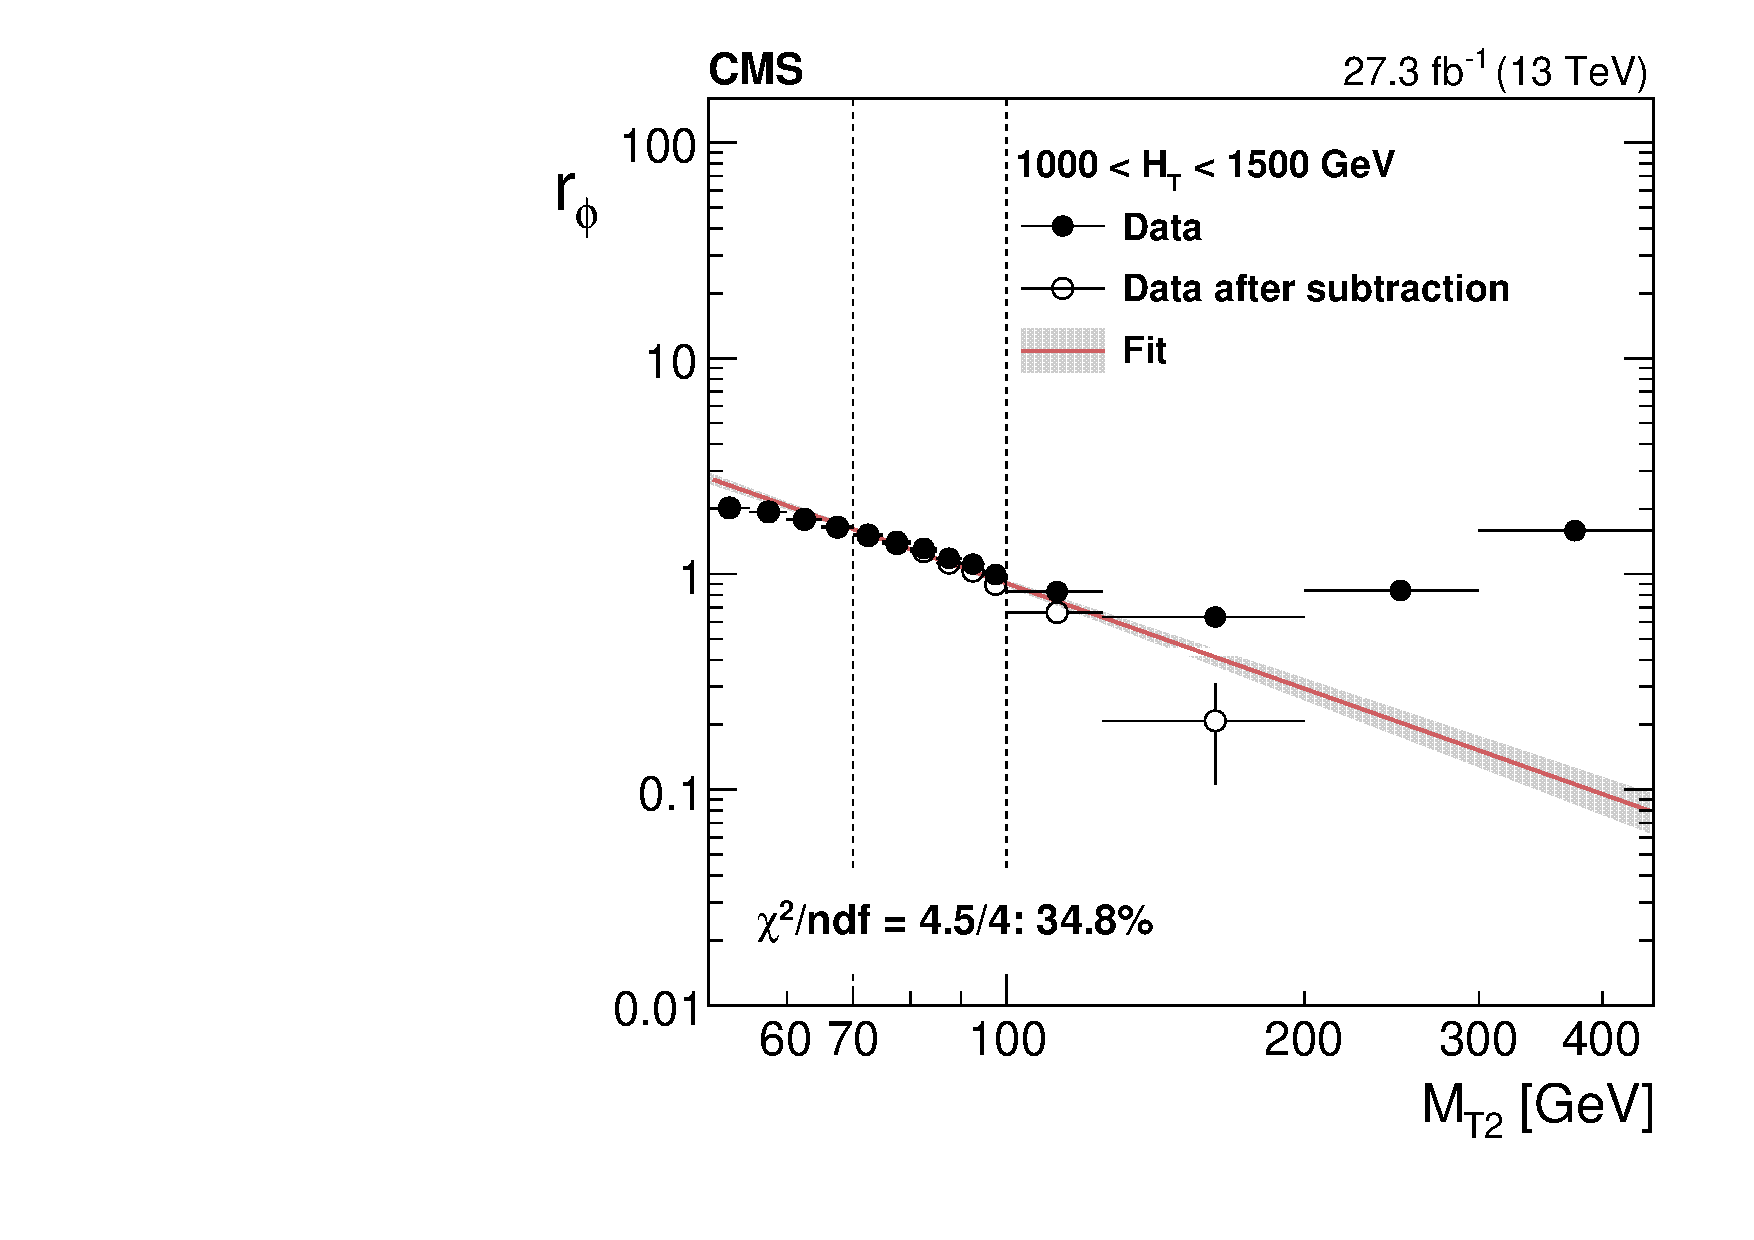
\includegraphics[width=0.85\textwidth]{figures/mt2_rphi_2016.pdf}
      \caption[Fit of $r_{\phi}$ as a function of \mttwo.]{
        The fit of $r_{\phi} = N_{\dphimin > 0.3}/N_{\dphimin < 0.3}$ as a function of \mttwo obtained in the 2016 classic search, for the $1000 < \Ht < 1500$~GeV \Ht band. 
        The fit is performed in events in the \mttwo band $70 < \mttwo < 100$~GeV and extrapolated to the $\mttwo > 200$~GeV signal region.
        Black points represent raw data, while white points represent data after the non-multijet contribution is subtracted.
        Taken from \cite{MT2_2016}.}
      \label{fig:rphi}
    \end{figure}  

    In older versions of the classic search \cite{MT2_2015, MT2_2016}, the mismeasurement background estimate used the \dphimin observable and extrapolated across \mttwo.
    Events at low \mttwo and at low \dphimin are both dominated by QCD mismeasurement.
    The suppression effect of \mttwo is so strong that even events at low \mttwo and {\it high} \dphimin are QCD dominated.
    As essentially every low \mttwo event is a QCD event, low \mttwo events can be used to measure the ratio $r_{\phi}$ of QCD mismeasurement events at high and low \dphimin.
    High \mttwo events with low \dphimin can then serve as a control region for estimating the QCD mismeasurement background, $N_{\dphimin > 0.3} = r_{\phi} N_{\dphimin < 0.3}$.
    Unfortunately, $r_{\phi}$ decreases with increasing \mttwo, so that instead the dependence must be fit to a power law at low \mttwo and extrapolated to high \mttwo, as shown in Figure~\ref{fig:rphi}.
    This procedure has obvious potential for statistical errors in the fit, systematic error in extrapolating the fit to high \mttwo, and potential non-multijet contamination of the low \dphimin control region at high \mttwo, producing total relative error at least 40\% and as large as 180\%.
    Although the impact of these errors is controlled by suppressing the mismeasurement background as described in Section~\ref{sec:MT2QCD}, it is desirable to replace this procedure with a more robust one.

    \begin{figure}[h!]
      \centering
      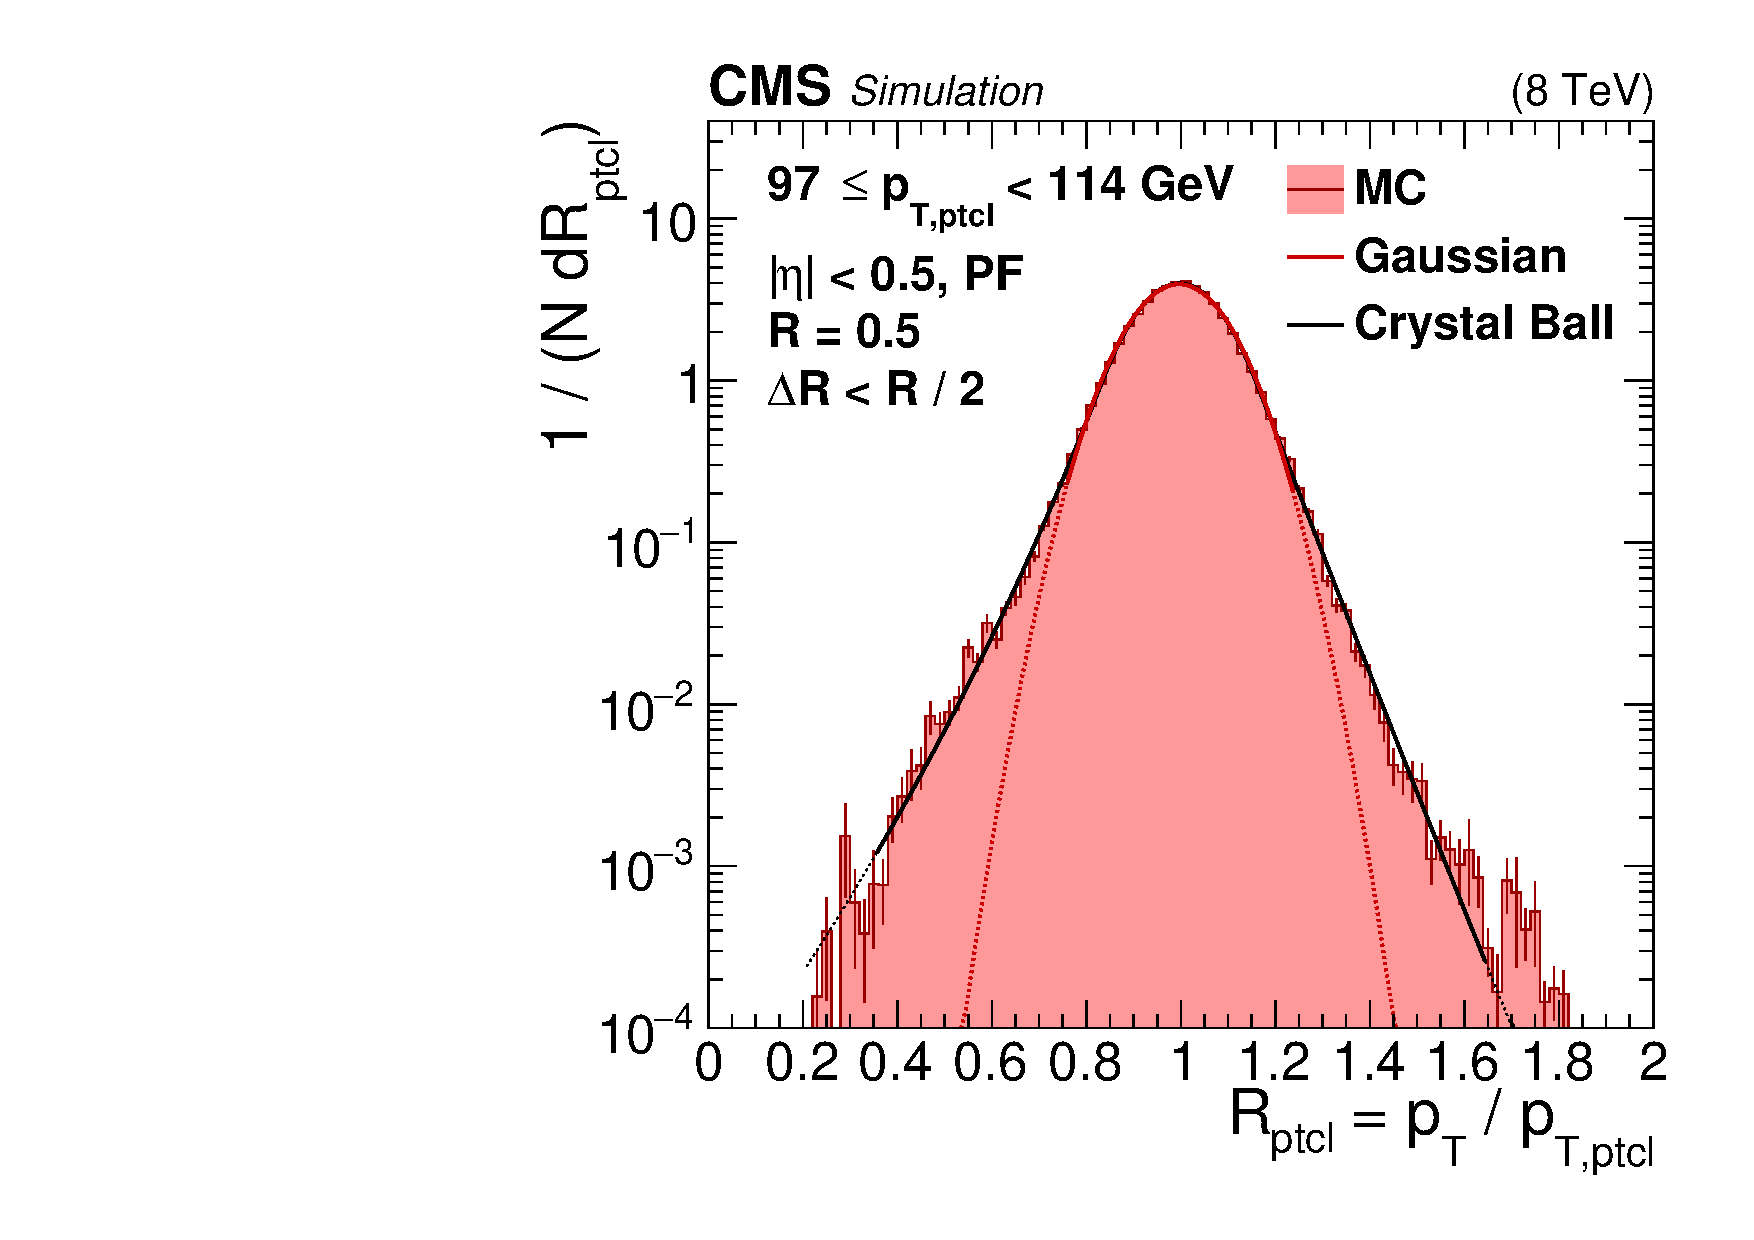
\includegraphics[width=0.85\textwidth]{figures/jet_resolution.pdf}
      \caption[Example plot of jet energy resolution template.]{
        $\mathrm{p}_{\mathrm{T,ptcl}}$ is the ``particle level'' \pt, the total energy that the jet's particle components actually had, while \pt is the energy measured by the detector.
        The horizontal axis is the ratio of these two quantities, and the vertical axis the probability that a jet's measured energy will differ from its true energy by that ratio.
        The response curve shown here applies to jets with particle level \pt in the band $97 < \pt < 114$~GeV, and measured in the CMS barrel.
        Large mismeasurements of jet energy are much less probable than small mismeasurements.
        The core is well-described by a Gaussian, but the tails are highly non-Gaussian and best described by a Crystal-Ball function.
        Taken from \cite{jet_resolution}.}
      \label{fig:jet_resolution}
    \end{figure}  


    Rebalance and Smear (R\&S) achieves the desired improvement.
    R\&S begins with a sample of multijet events from data with \Ht on the order of hundreds of GeV and at least two jets with $\pt > 10$~GeV.
    This is as nearly unbiased a sample of QCD events as is allowed by available triggers.
    These events will generically have some small but nonzero \met due to imperfect measurement of the jet energies, dictated by the detector's resolution, jets from pileup, very low energy objects in the event, and potentially a very small contribution from genuine neutrinos produced in the hadron decay chains inside the jets.
    The \pt values assigned to the jets are then adjusted, finding the most likely assignment of \pt values subject to the hypothesis that the true \met is very nearly zero, and that jet mismeasurements of a given size occur with probability given by jet response templates.
    As shown in Figure~\ref{fig:jet_resolution}, large mismeasurements are rare.
    Thus, the Rebalancing step tries to get the \pt as close to zero as feasible without making more improbable adjustments to the jets than necessary.
    The output of the Rebalancing step is a large sample of real QCD events with maximally accurate jet \pt assignments.

    Then, each of these events goes through a Smearing step.
    This step randomly assigns a new \pt to each jet in the event according to the same jet response templates.
    The vast majority of the time, the new event looks as unremarkable as the original event before Rebalancing.
    Rarely, the output event passes the baseline selection and represents a potential mismeasurement event that might lie in the data signal region.
    The Smearing can be repeated as many times for each event as is desired, subject to computing limitations.
    The number of Smeared events falling into each signal region, from this sample of known equivalent integrated luminosity, can then be converted into the expected number of events that would fall into the signal region in data, due to jet mismeasurement.
    
  \begin{figure}[h!]
    \centering
    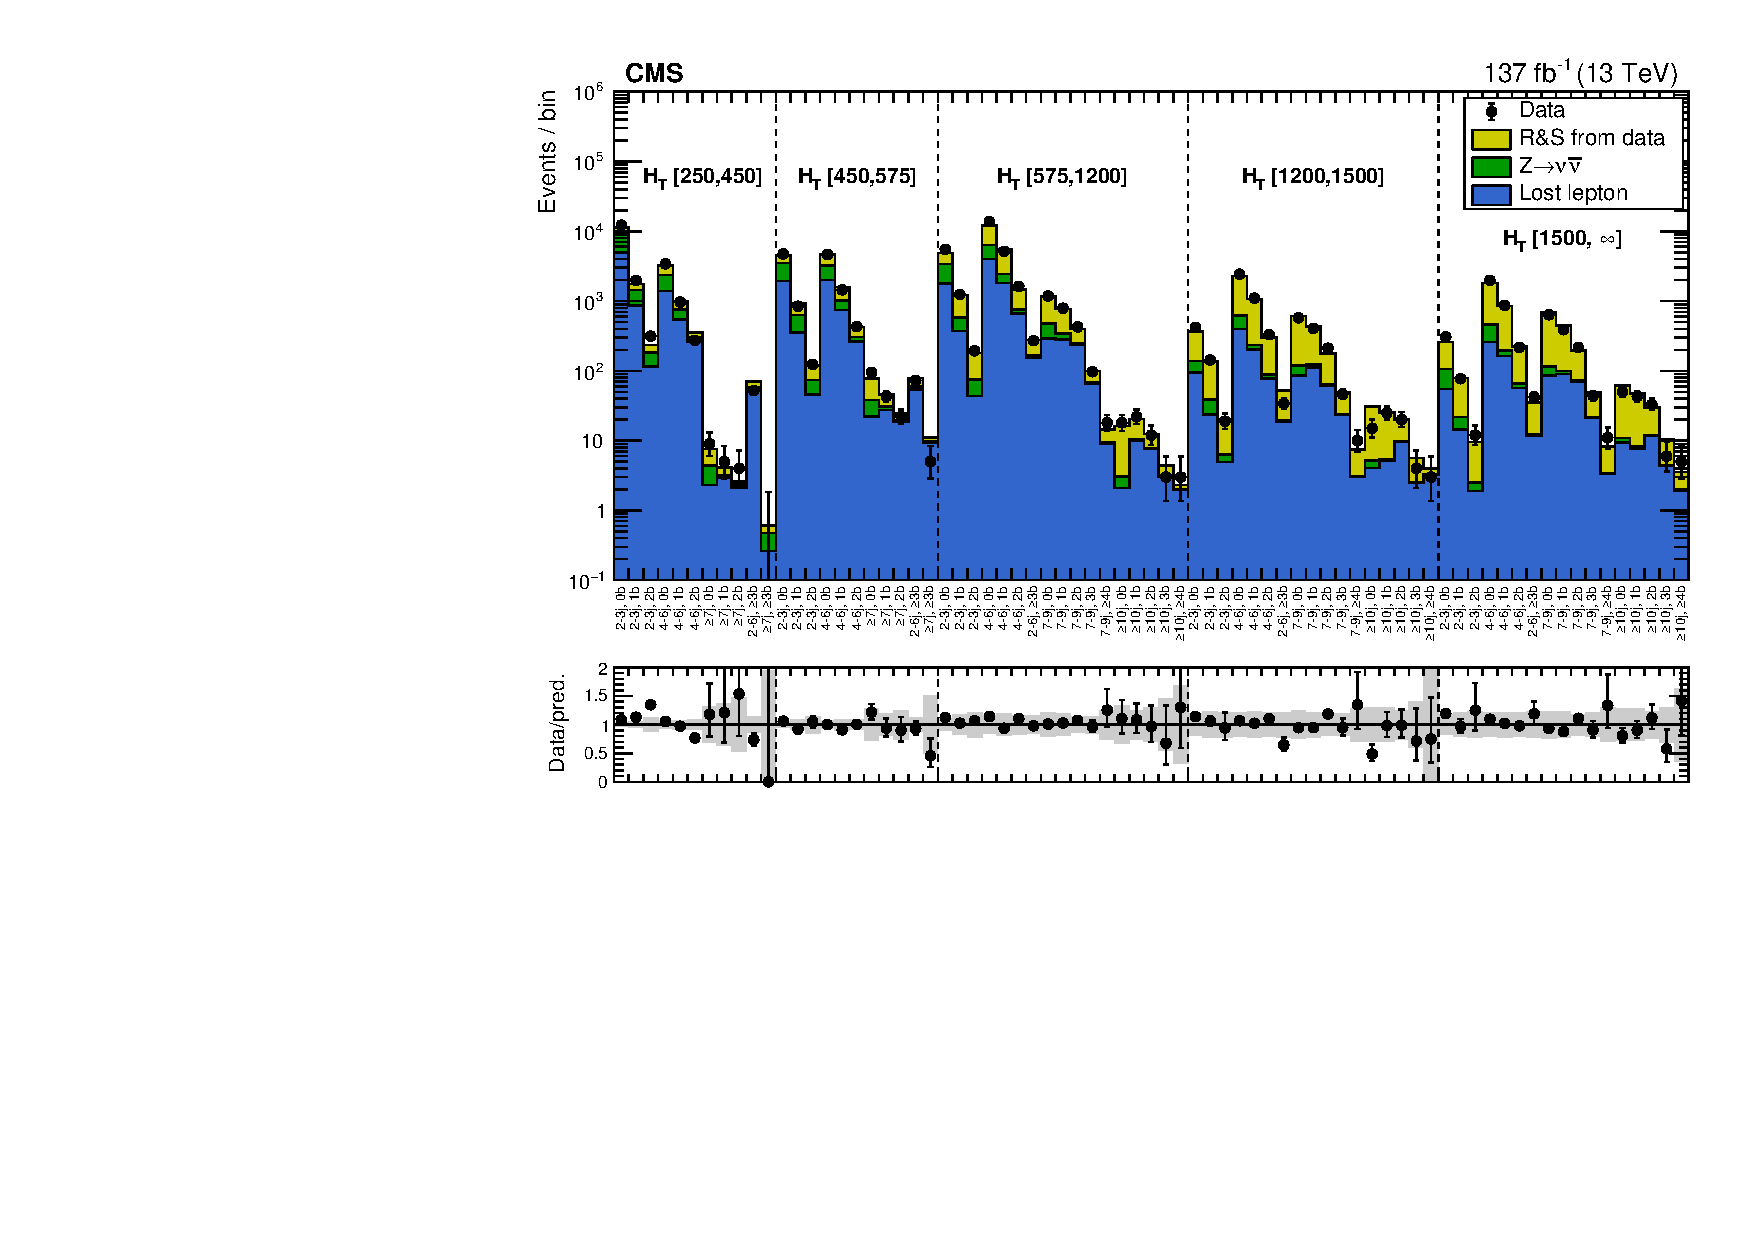
\includegraphics[width=0.85\textwidth]{figures/MT2_2019/Figure_003.pdf}
    \caption[Validation of the Rebalance and Smear jet mismeasurement background estimate in the $\dphimin < 0.3$ control region.]{
      The Rebalance and Smear jet mismeasurement background estimate is validated in the $\dphimin < 0.3$ control region. 
      The multijet mismeasurement event count predicted by Rebalance and Smear is shown in yellow, and contributes most of the event counts in this control region. 
      The combined background estimate (filled histogram) is consistent with the data observation (black data points).
      Taken from \cite{MT2_2019}.}
    \label{fig:RandSval}
  \end{figure}  

    Of course, many of the output events will have $\dphimin < 0.3$, falling outside of the signal region into the QCD-dominated low $\dphimin$ control region.
    This allows for a validation in data of the R\&S procedure, shown in Figure~\ref{fig:RandSval}.
    The total background estimate is consistent with data in the $\dphimin < 0.3$ control region across all of the analysis bins, with the R\&S estimated counts contributing most of the predicted events.

    \begin{table}[tbhp]
      \centering
      \topcaption[Systematic uncertainties affecting the Rebalance \& Smear jet mismeasurement background estimate.]
                 {\label{tab:qcdsyst}
                   Summary of systematic uncertainties in the multijet background prediction,
                   together with their typical size ranges across the search bins.
                   ($\dagger$) The parameter $\sigma_\text{T}^{\text{soft}}$ is the width of the assumed underlying irreducible \met distribution for a multijet event, used as an input to the Rebalancing step, and so-called because such \met is dominated by low energy objects.
                   The final output is largely independent of the precise choice for this parameter and the shape of the underlying distribution, but a systematic is assessed to cover any observed variations.
                   Taken from \cite{MT2_2019}.
      }
      \begin{tabular}{ l  c }
        \hline
        Source & Range [\%] \\
        \hline
        Jet energy resolution & 10--20\\
        Tails of jet response in templates & 17--25\\
        $\sigma_\text{T}^{\text{soft}}$ modeling$^{\dagger}$ & 1--25\\
        \njet modeling & 1--19\\
        \nb modeling & 1--16\\
        \hline
      \end{tabular}
    \end{table}

    R\&S achieves a significant improvement over the old $r_{\phi}$ based system, effectively eliminating statistical error, and improving the worst case relative error on the mismeasurement estimate from 180\% to less than 50\%.
    Systematic uncertainties are summarized in Table~\ref{tab:qcdsyst} together with their typical size ranges across the search bins.
    The sources of these uncertainties are described either in the text above, or are shared with the uncertainties affecting the genuine neutrino backgrounds.

    \subsubsection{Expanded Binning} \label{sec:newbinning}

    Although the baseline selection defines the class of events in which a signal of interest may be found, most signals will produce a significant number of events in only a subset of the phase space.
    For instance, a signal producing 4 top quarks in the final state (see Figure~\ref{fig:susyproduction} second row, right) will almost always produce events with $\njet \geq 7$, $\nb > 0$, and $\Ht \sim 1$~TeV.
    If the entire set of selected events is considered together, the entire background is combined, potentially hiding a signal.
    If instead the phase space is divided into many separate regions, the background in each region is smaller, so that the background count is as small as possible in the small subset of regions that any given signal actually populates.
    This sensitivity enhancement motivates very fine binning of the signal region.
    The classic search uses \mttwo, \Ht, \njet, and \nb as binning variables.

    In the 2016 version of the classic search \cite{MT2_2016}, the most extreme \njet\xspace bin was $\njet \geq 7$, and the most extreme \nb bin was $\nb \geq 3$.
    This limitation was imposed by limited statistics.
    The background estimate for each bin is performed separately, and the observed counts are subject to Poisson statistical flucuations.
    Binning too finely causes any potential sensitivity gains from better isolating signal to be lost to greater uncertainty in the expected background.
    The analysis binning was updated for the latest edition of the classic search \cite{MT2_2019}, anticipating the improved statistical power.
    The full set of new bins, along with the predicted background counts and observed event counts in data, is available in Appendix~\ref{app:classicbinning}.

    The new binning extends the old binning in three ways.
    First, new $\njet \geq 10$ bins were added to the $\Ht > 1200$~GeV regions.
    This allows for enhanced sensitivity to signals with extremely high jet multiplicity, such as the 4 top signal previously mentioned.
    Similarly, new $\nb \geq 4$ bins were added to these same regions, targeting the same signal.
    Sensitivity to some mass points of this signal model roughly doubled due to the addition of these bins, which have negligible background but appreciable signal counts.
    Finally, \mttwo binning was generally made narrower and the last bin moved to larger \mttwo values, for all signal regions, until the expected background in the last bin was on the order of 1 event.
    In all, there are 282 classic search bins, enhancing sensitivity to a broad array of potential signal models.

  \subsection{Signal Contamination} \label{sec:MT2sigcontam}

  The data driven estimate procedures for the neutrino backgrounds used control regions defined using leptons.
  Signals capable of producing leptons can contaminate these control regions, increasing the observed control region counts above the actual Standard Model production rate.
  This leads directly to an overprediction of background.
  For instance, consider stop pair production followed by decay to tops, as shown in Figure~\ref{fig:susyproduction} (row 3, right).
  Both tops will decay to a W and a bottom quark.
  If one of the W bosons decays leptonically and the lepton is reconstructed, the event will likely enter the single lepton control region.
  The lost lepton background, described in Section~\ref{sec:MT2lostlep}, will be overpredicted,
  \begin{equation}
    N_{LL}^{\mathrm{Data;Est}} = R_{MC}^{0\ell/1\ell} N_{SL}^{\mathrm{Data}} = R_{MC}^{0\ell/1\ell} \left(N_{SL}^{\mathrm{Data;SM}} + N_{SL}^{\mathrm{Data;BSM}}\right).
  \end{equation}
  The background overprediction is $\Delta N = R_{MC}^{0\ell/1\ell}N_{SL}^{\mathrm{Data;BSM}}$.
  For analysis purposes, the overprediction is modeled in simulation and treated as a reduction of the expected signal counts in every affected bin.
  \begin{equation}
    N_{SR}^{\mathrm{BSM;Adjusted}} = N_{SR}^{\mathrm{BSM;Raw}} - \Delta N
  \end{equation}
  This adjustment has the nice property that all terms are linear in the signal strength, so that it does not need to be recalculated for every signal strength considered when performing statistical analysis of the results.
  The same fraction of the signal is lost at every signal strength.
  
  As a result of this loss of sensitivity due to signal contamination, the classic analysis is less effective, all things equal, when used to search for signals that sometimes produce leptons than the naive expectation based on the leptonic versus hadronic branching ratios.
  This is an inevitable consequence of performing an all-hadronic search.

  \subsection{Results} \label{sec:MT2results}

  \begin{figure}[h!]
    \centering
    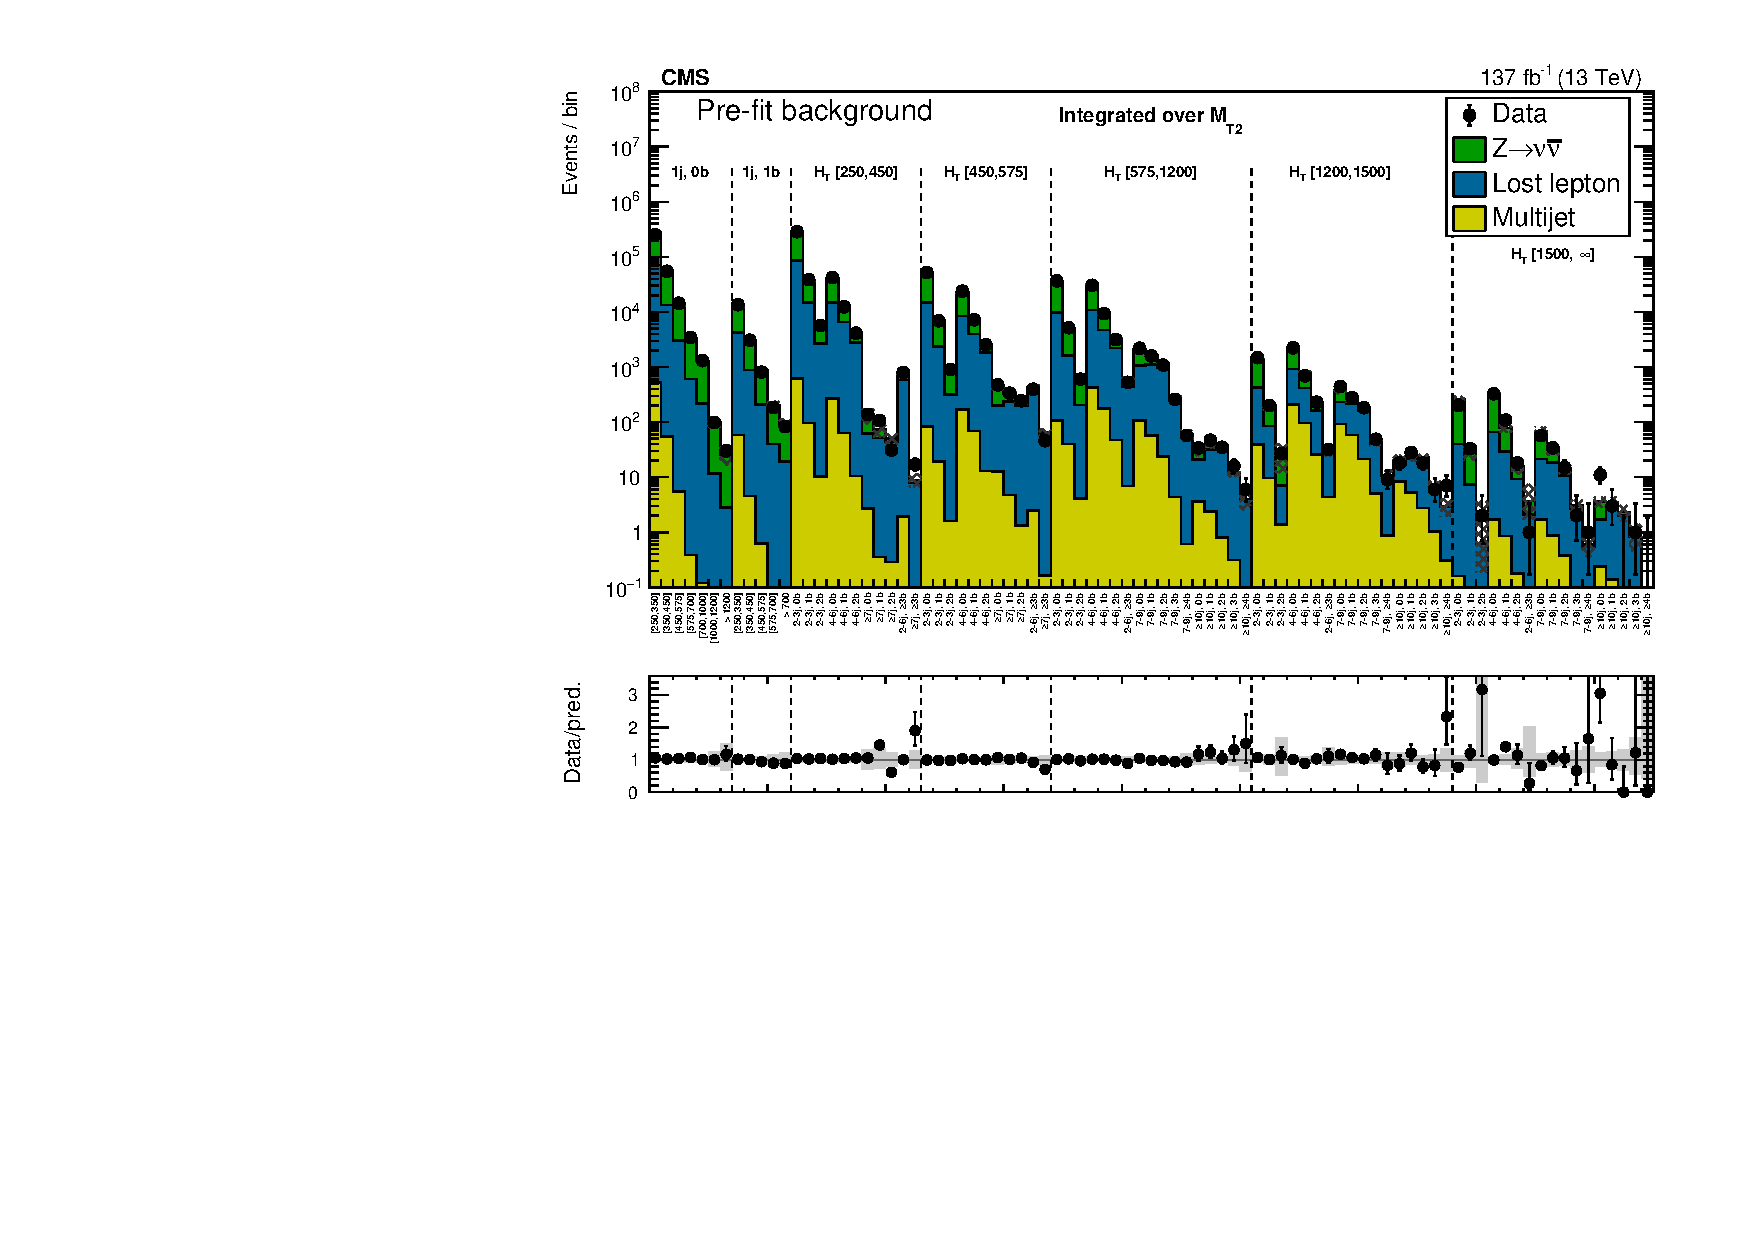
\includegraphics[width=0.85\textwidth]{figures/MT2_2019/Figure_005-a.pdf}
    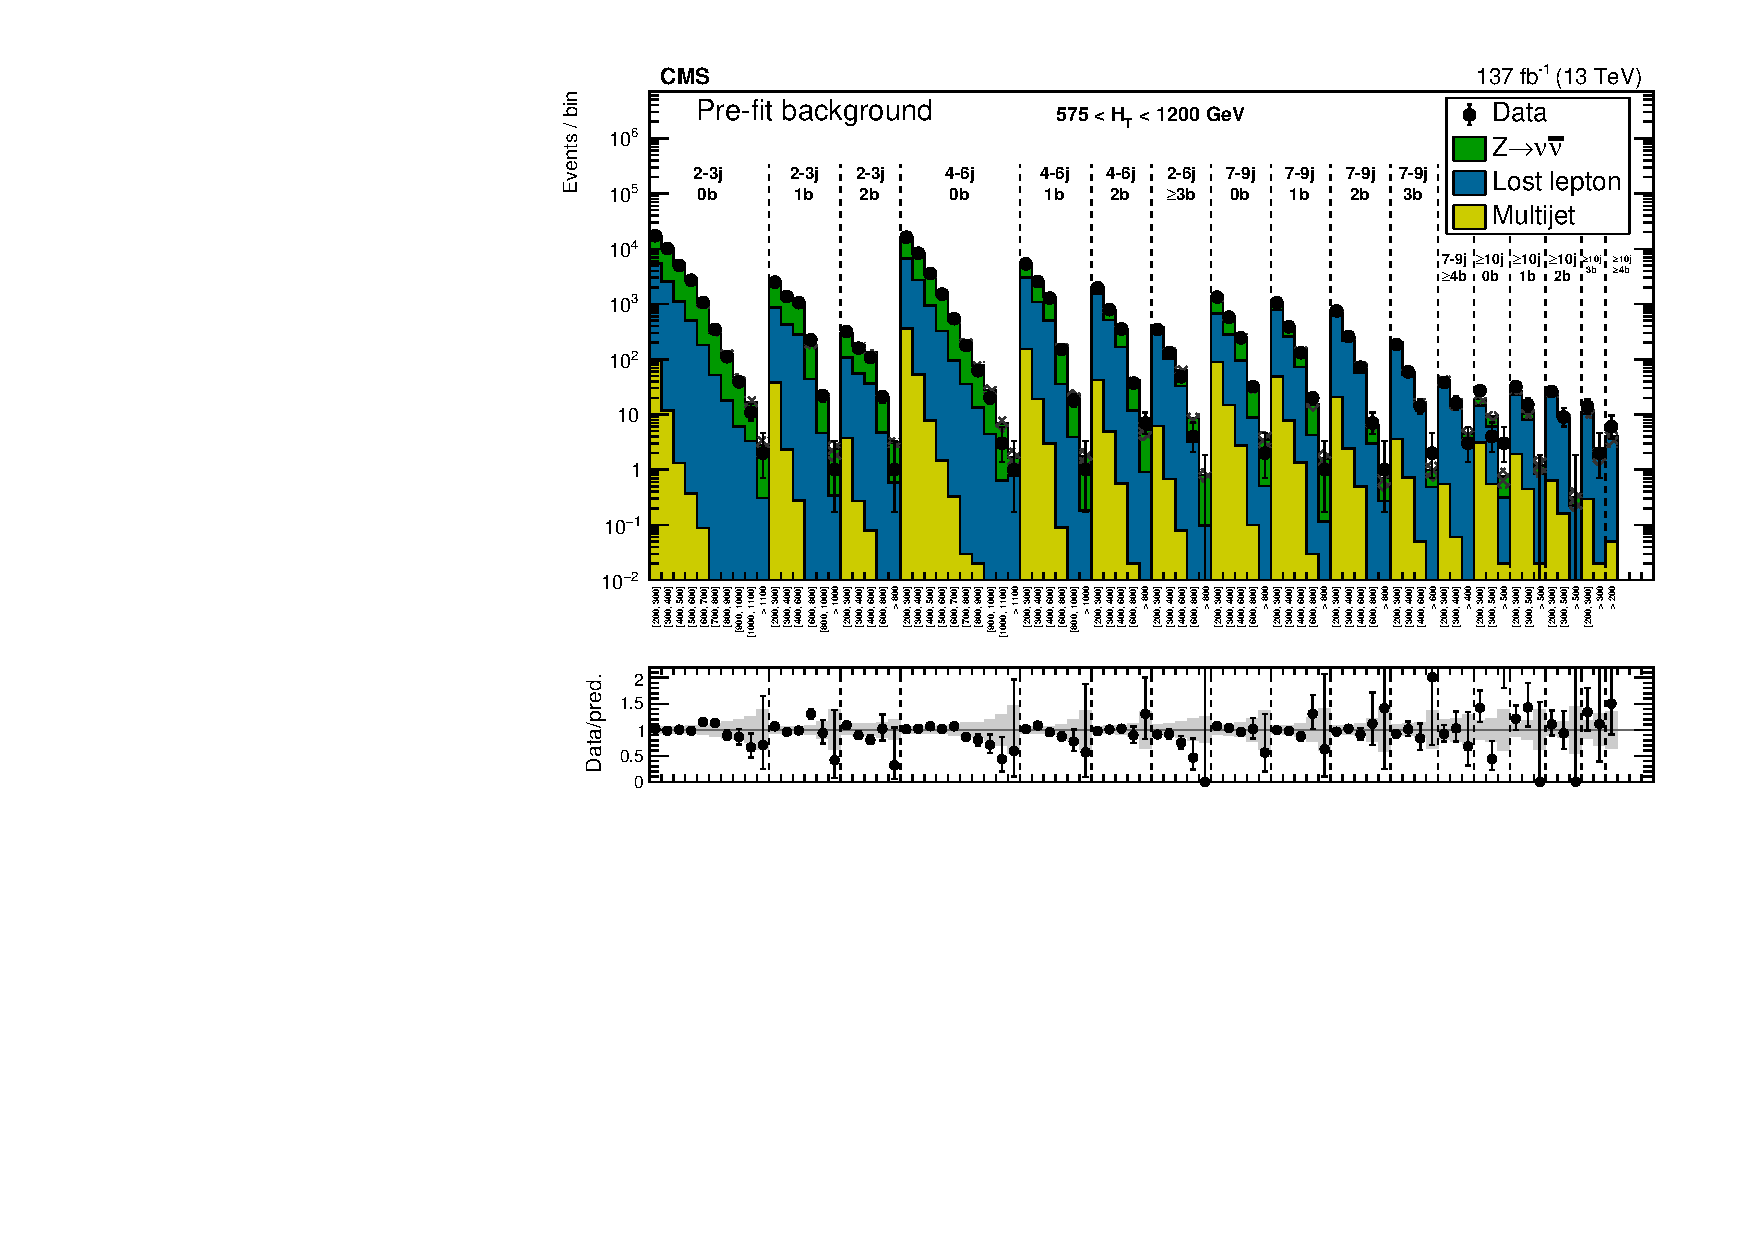
\includegraphics[width=0.85\textwidth]{figures/MT2_2019/Figure_005-b.pdf}
    \caption[Comparison of predicted background and observed data events in the classic search (upper) integrated over \Mttwo and (lower) for each of the medium \Ht search regions.]{Comparison of predicted background and observed data events in the classic search (upper) integrated over \Mttwo and (lower) for each of the medium \Ht search regions. Taken from \cite{MT2_2019}.}
    \label{fig:classicresults}
  \end{figure}  

  The full set of results for every classic search signal region, including every background prediction and the observed count, are available in Appendix~\ref{app:classicbinning}.
  The full set of results integrating over the \mttwo binning are display in Figure~\ref{fig:classicresults} (upper), and the results including the \mttwo binning for the $575 < \Ht < 1200$~GeV bins, the largest set, are shown in Figure~\ref{fig:classicresults} (lower).
  The observed counts are consistent with the background-only hypothesis, and the results are used to set exclusion limits at 95\% confidence level on the signals discussed in Section~\ref{sec:MT2sig}.

  \subsection{Limits} \label{sec:MT2limits}

  The \CL statistical analysis procedure is decribed in \cite{CLS_method}.
  It begins with maximum likelihood fits to the background-only and signal-plus-background hypotheses, for each signal model, considering each mass point separately. 
  The likelihoods are products of Poisson probabilities for each signal region bin, with log-normal constraint terms for each systematic affecting the predicted counts.
  Correlation between uncertainties affecting different bins are fully accounted for.
  As stated in the previous section, the background-only hypothesis is consistent with the observation.
  So, the parameter of interest for each signal model is the maximum signal cross section that can be excluded with 95\% confidence level.
  That is, the maximum possible production rate that the signal model could have, without requiring a combination of background and signal fluctuations more improbable than 1 in 20 to be consistent with the data.
  If the production cross section excluded at 95\% CL is less than the theoretical cross section for a given signal model, that signal model is said to be excluded at 95\% CL.

  The simplified supersymmetric extensions to the Standard Model shown in Figure~\ref{fig:susyproduction} have only two free parameters, the masses of the pair-produced superpartner, and the mass of the lightest supersymmetric particle, the dark matter candidate \lsp.
  Plotting the gluino or squark mass on the horizontal axis and the mass of \lsp on the vertical axis, then marking the mass points excluded at exactly 95\% CL, produces the exclusion curves shown in Figures~\ref{fig:t5x}--\ref{fig:stop_other}.
  Points to the lower left of these curves are excluded, while points above and to the right are not, as they require fluctuations no more improbable than 1 in 20 to be consistent with present data.

  The CMS dataset was collected only once, and this dataset is subject to fluctuations.
  The multiple exclusion curves shown on each plot, some in red and some in black, provide an indication of how unusual the limits generated by this dataset were.
  Suppose that the background's expected event count in a given region, summing across this entire dataset, is $B$.
  It is clearly possible that the actual number of background events that occur in the dataset in this bin could be around $B+\sqrt{B}$, or $B-\sqrt{B}$.
  In the first case, the analysis will draw unexpectedly strong limits on signals that populate this bin.
  In the second case, the analysis will draw unexpectedly weak limits on signals.

  The curves shown in red are the median, 1 standard deviation, and 2 standard deviation expected exclusion curves, in the background-only hypothesis.
  Together, these indicate the typical range of exclusion curves across many imaginary CMS datasets in which there is no signal to find.
  The curves in black are those that were observed in the CMS dataset as actually recorded.
  When the black observed curves extend out beyond the red expected curves, the analysis likely benefitted from a downward fluctuation of background.
  In cases where the observed curves swing inward compared to the expected curves, the analysis may have experienced an analogous unlucky upward fluctuation of background that mimicked a small signal, or alternatively there may be a genuine small signal lurking in the data that is resisting exclusion!

  The general shape of the curves is set by a combination of the falling cross section with increasing gluino or squark mass shown in Figure~\ref{fig:SUSYxsec}, and a loss of signal efficiency and signal versus background discriminatory power when the mass splitting between the gluino or squark and \lsp is small.
  On the lower right hand side of the plots lie signals that produce spectacular, energetic events, but at a very low rate due to the large mass of the gluino and squark, and accordingly small pair-production cross section.
  Moving up along the \lsp mass axis towards the upper right, the events remain spectacular, so the exclusion curves remain roughly vertical, limited only by the production cross section.
  Eventually, the mass splitting becomes small enough that the loss of signal efficiency and signal versus background discriminatory power becomes significant, and the exclusion curve turns to the left, towards lower mass squarks or gluinos and higher production rates.
  Decreasing the gluino or squark mass at fixed \lsp mass reduces the mass splitting, so the curve generally must also drop down somewhat along the \lsp mass axis to maintain a reasonable splitting.
  Eventually, the curve intercepts the $M_{\lsp} = M_{\tilde{g}}$ or $M_{\lsp} = M_{\tilde{q}}$ line.
  At this mass and below, all points are excluded even in the limit of zero mass splitting.


\begin{figure*}[htbp]
  \centering
    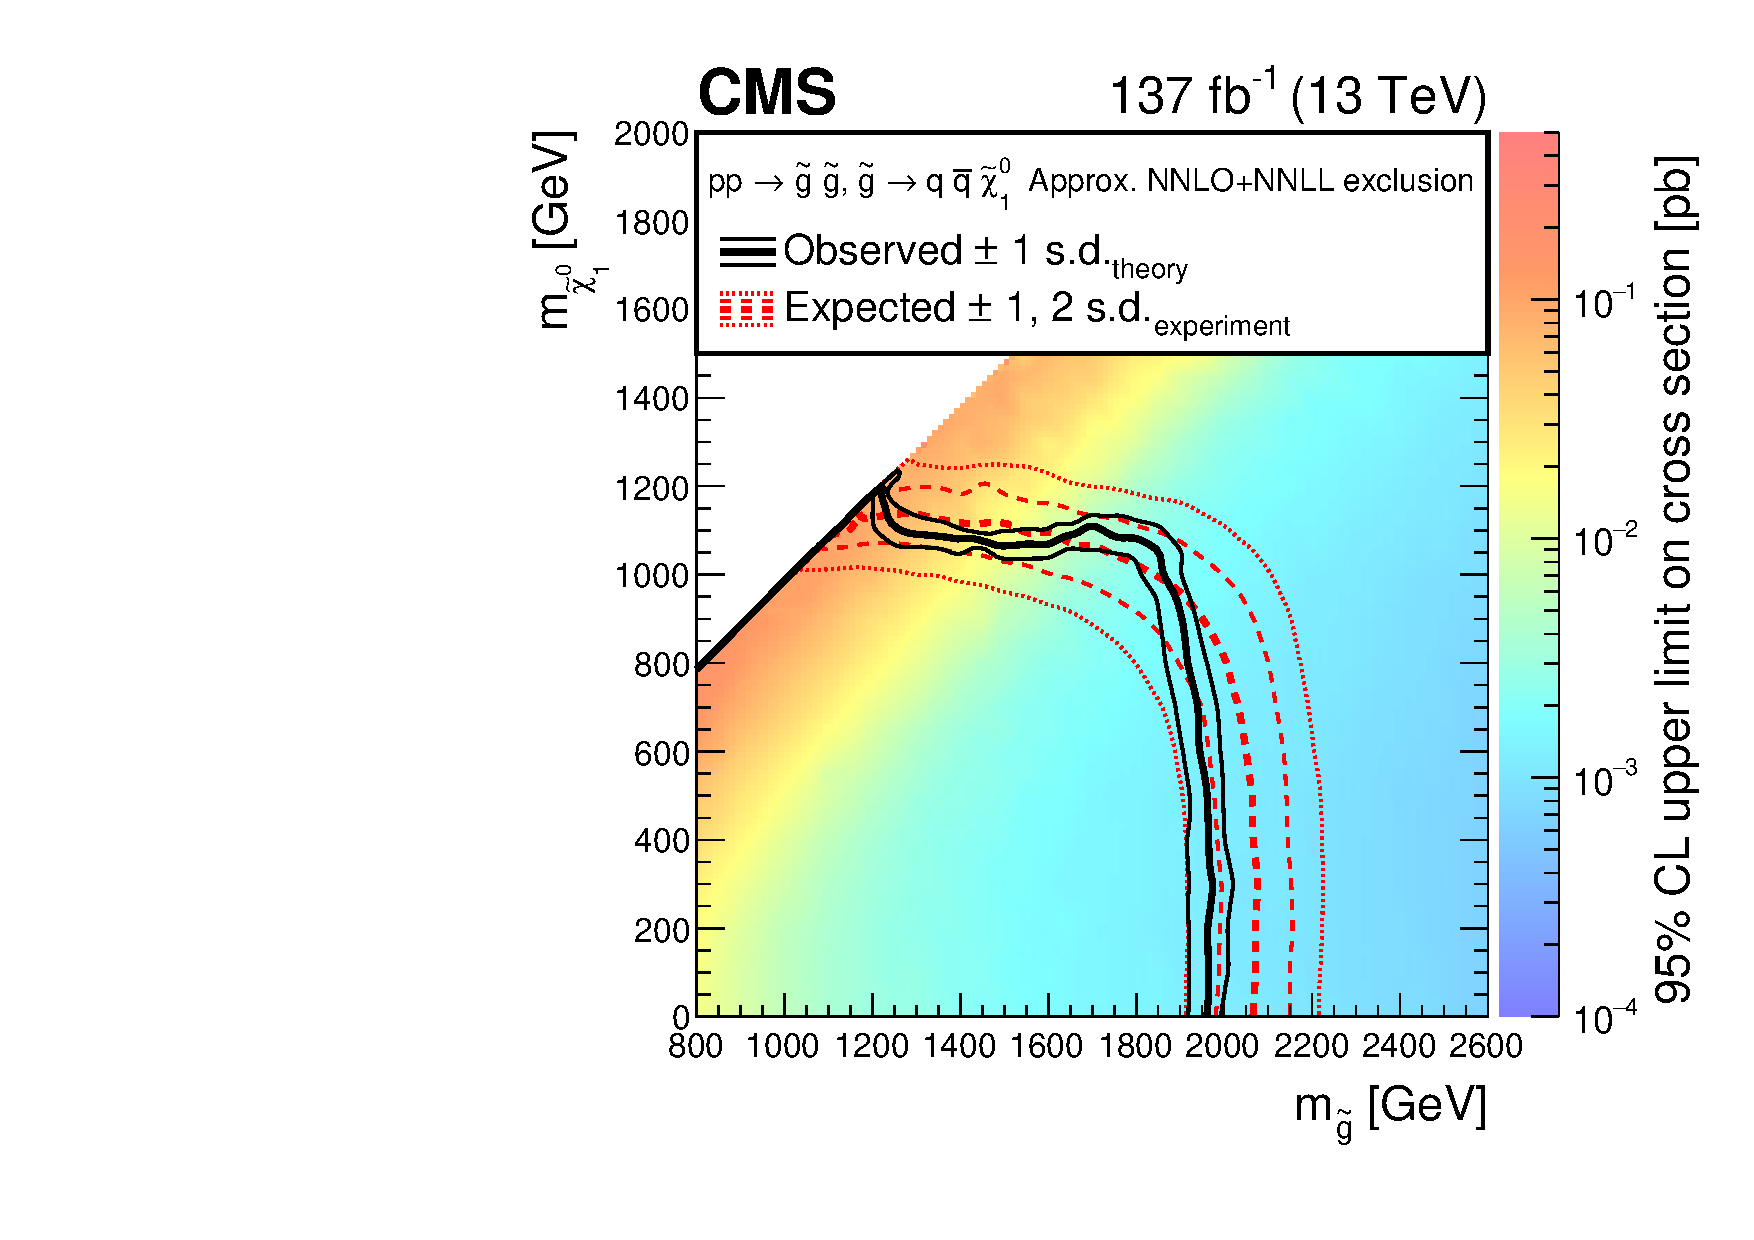
\includegraphics[width=0.48\textwidth]{figures/MT2_2019/Figure_011-a}\\
    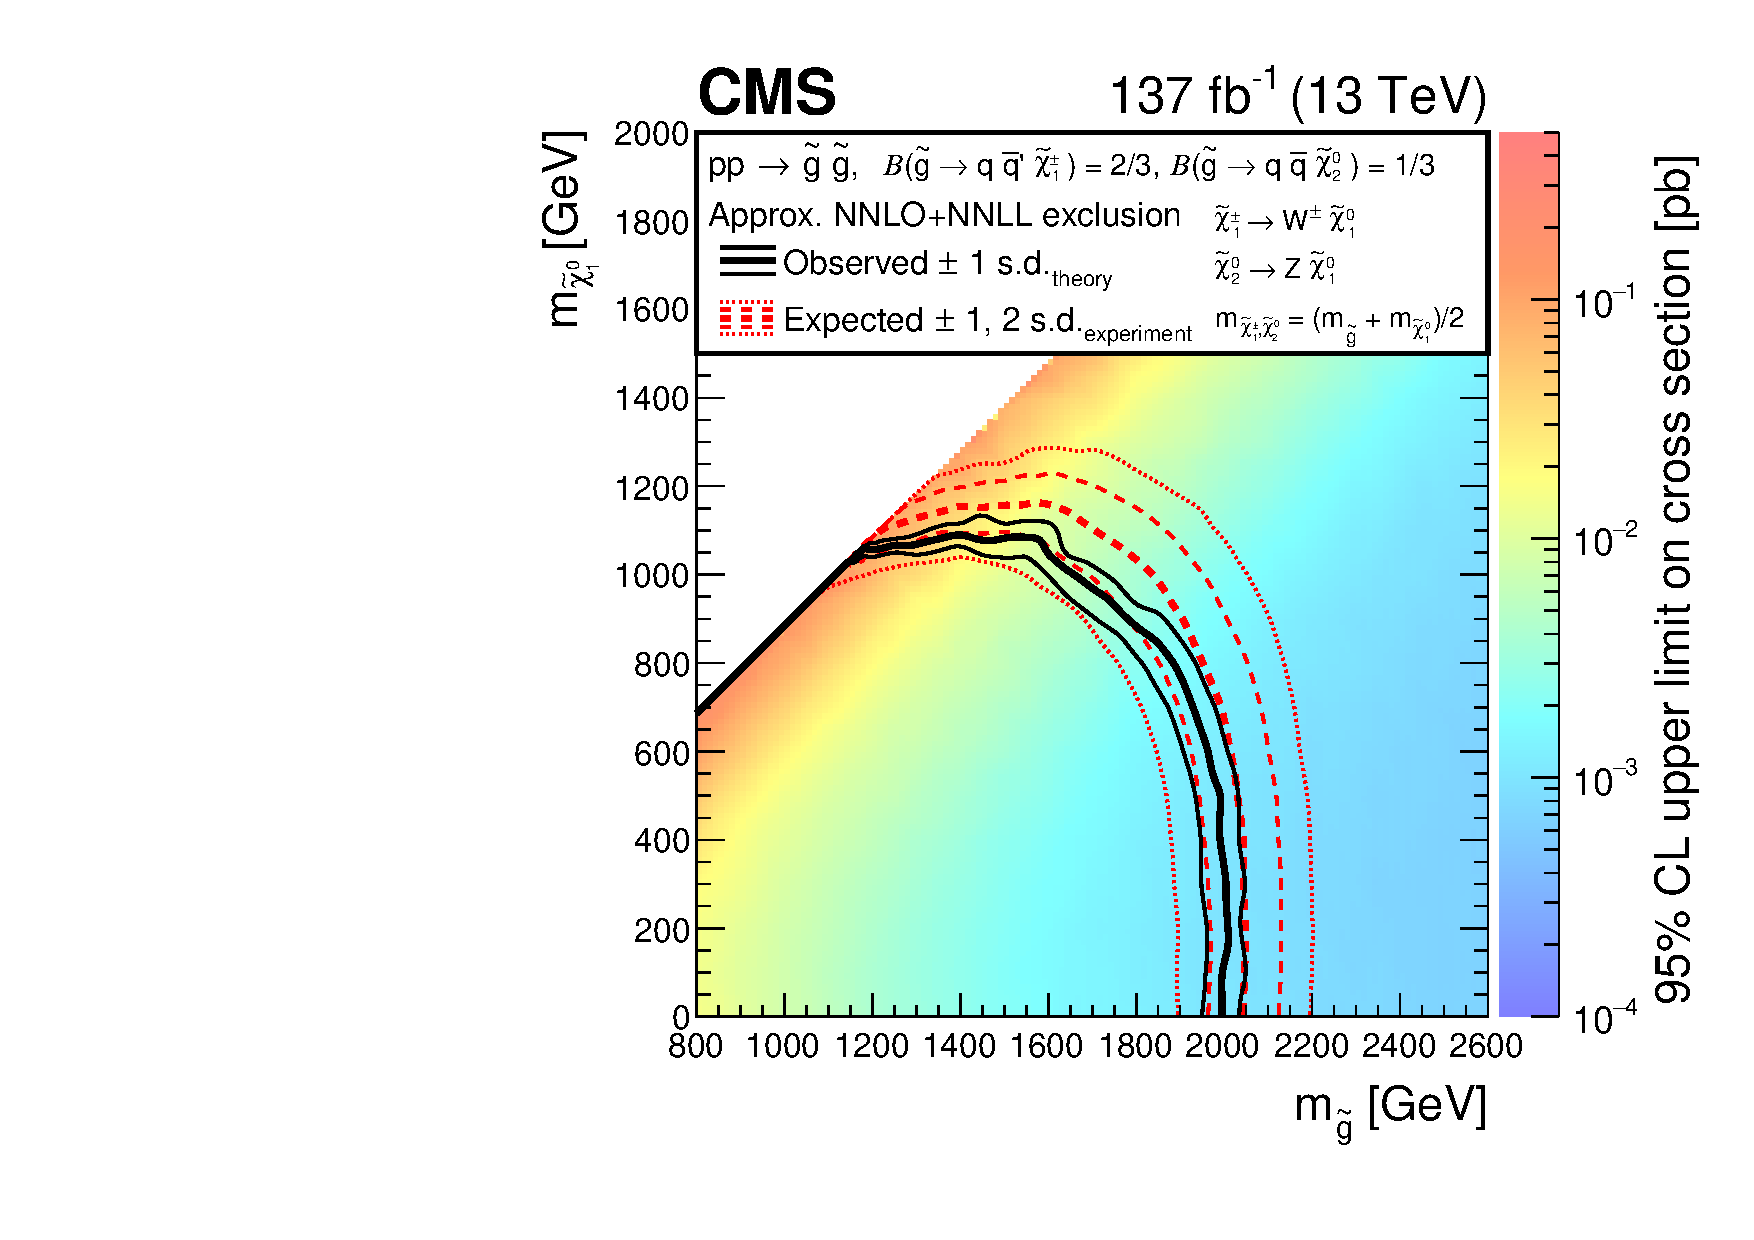
\includegraphics[width=0.48\textwidth]{figures/MT2_2019/Figure_011-b}
    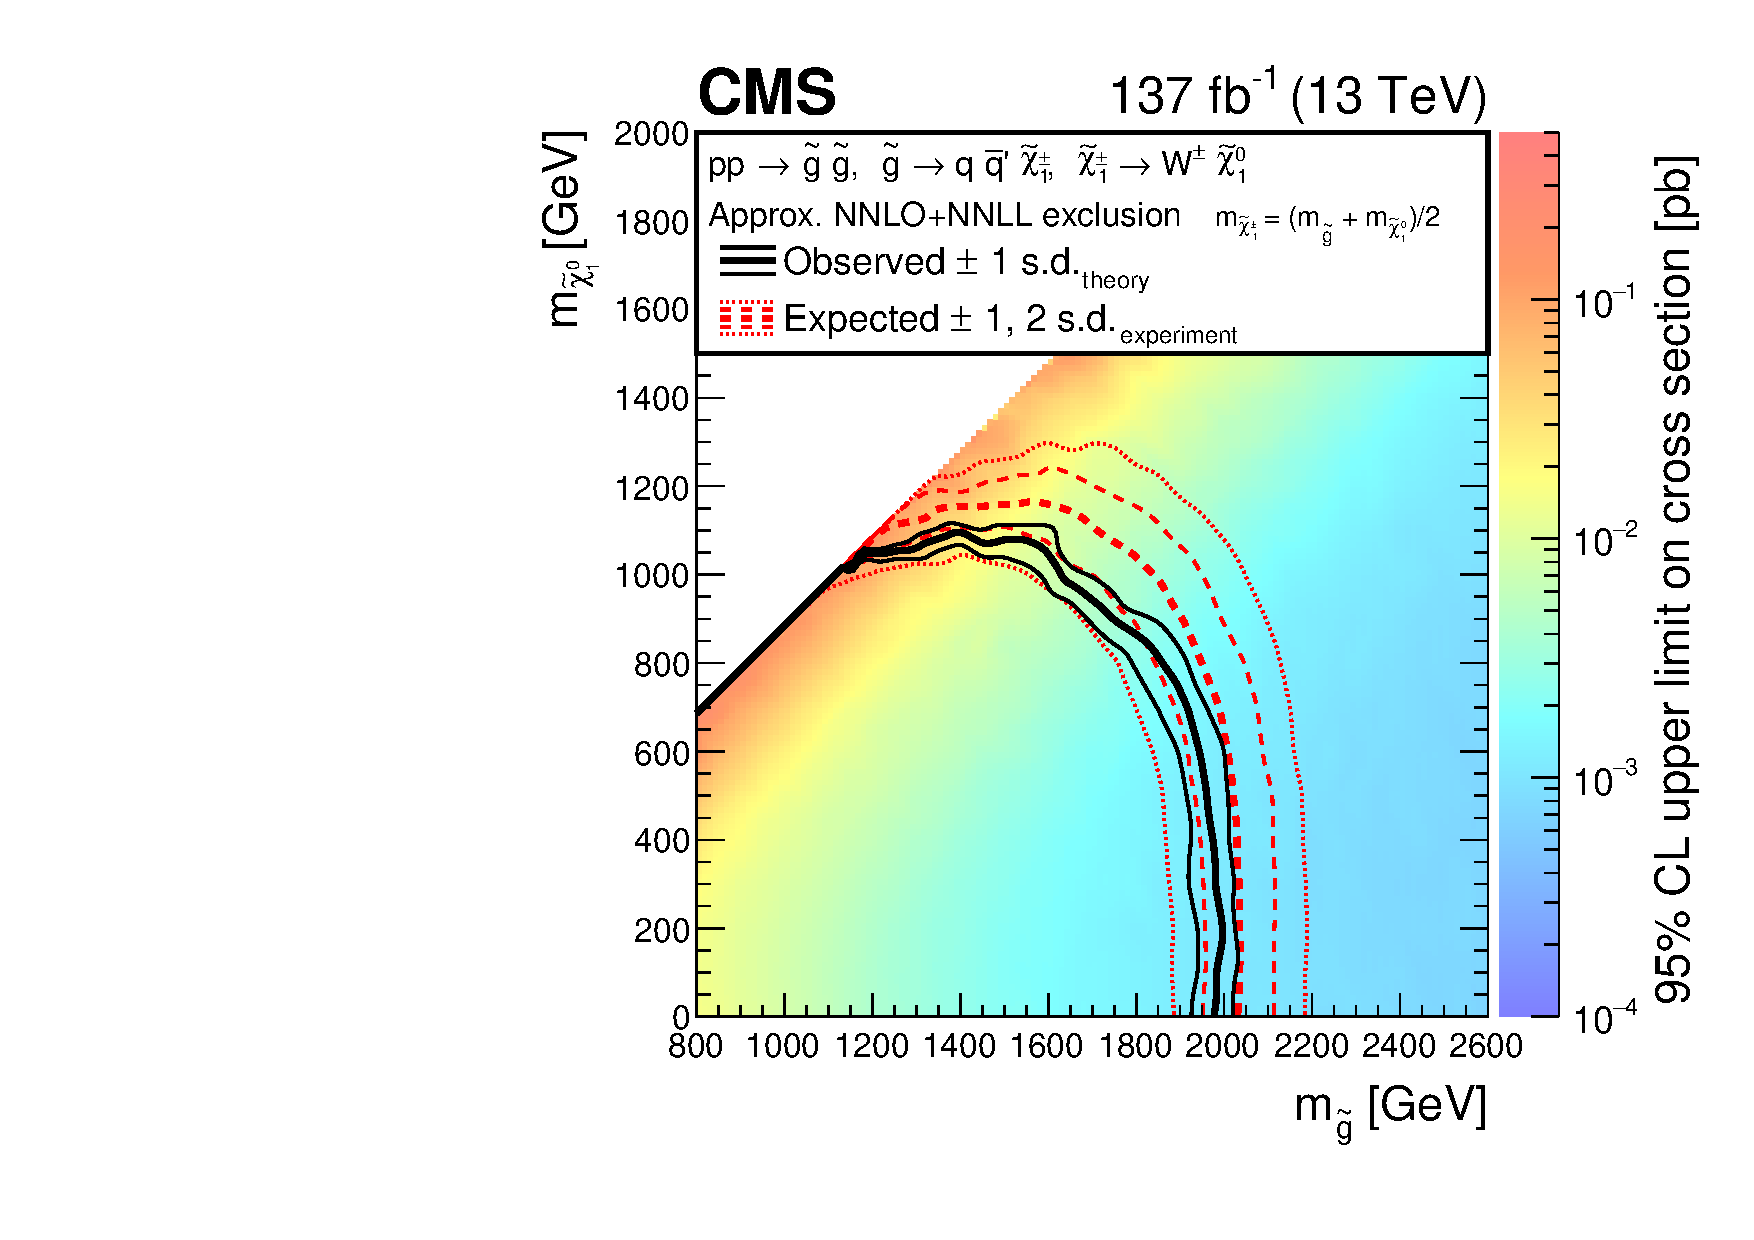
\includegraphics[width=0.48\textwidth]{figures/MT2_2019/Figure_011-c}
    \caption[Exclusion limits for gluino pair production and decay to light quarks.]{Exclusion limits at 95\% \CL for gluino pair production and decay to a pair of light quark jets and (upper) \lsp, (lower left) a democratic split between \lsp, \chitwo, which then decays to a Z boson and \lsp, and \chargino, which decays to a W boson and \lsp, and (lower right) \chargino then W and \lsp with 100\% branching fraction. Taken from \cite{MT2_2019}.}
    \label{fig:t5x}
\end{figure*}

\begin{figure*}[htbp]
  \centering
    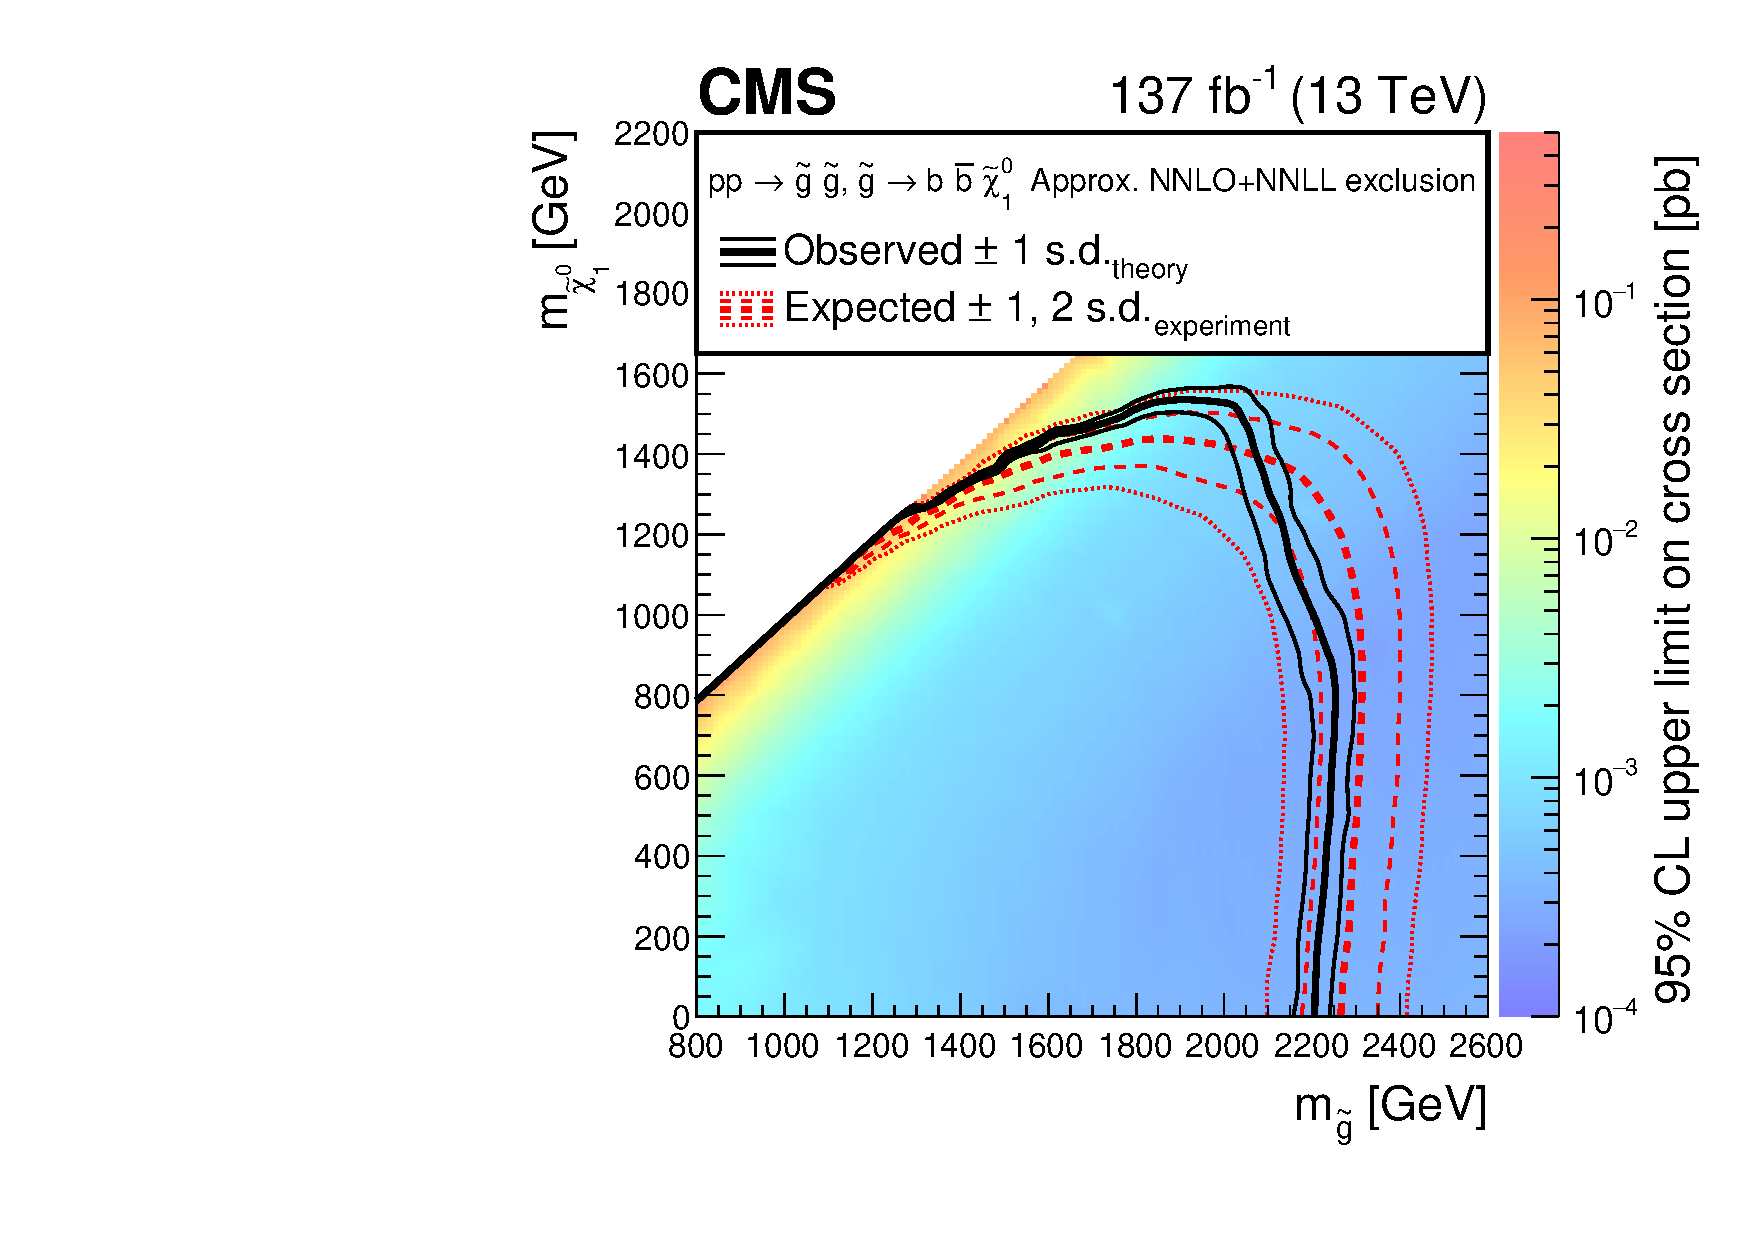
\includegraphics[width=0.48\textwidth]{figures/MT2_2019/Figure_012-a}
    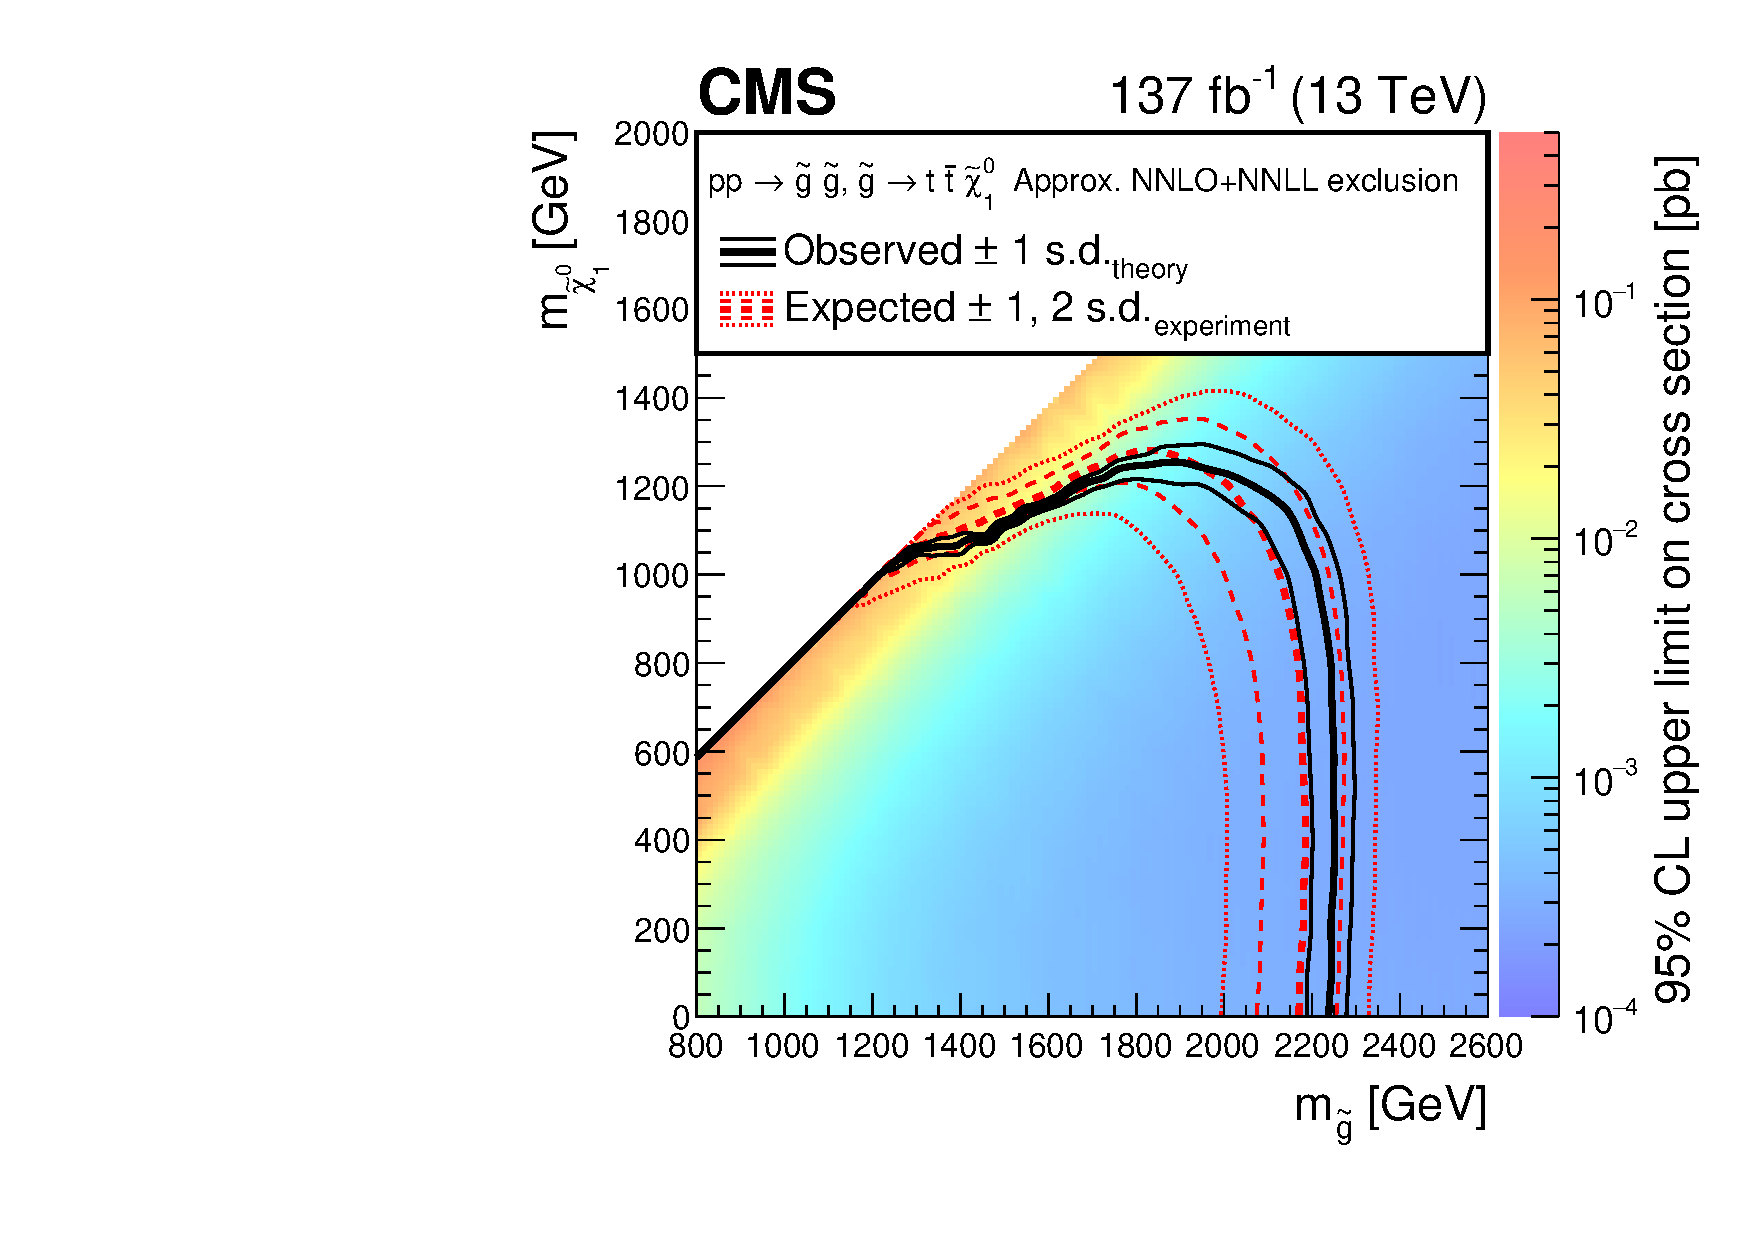
\includegraphics[width=0.48\textwidth]{figures/MT2_2019/Figure_012-b}
    \caption[Exclusion limits for gluino pair production and decay to bottom (left) and top (right) quarks.]{Exclusion limits at 95\% \CL for gluino pair production and decay to (left) bottom quarks and (right) top quarks. Taken from \cite{MT2_2019}.}
    \label{fig:t1x}
\end{figure*}

\begin{figure*}[htbp!]
  \centering
    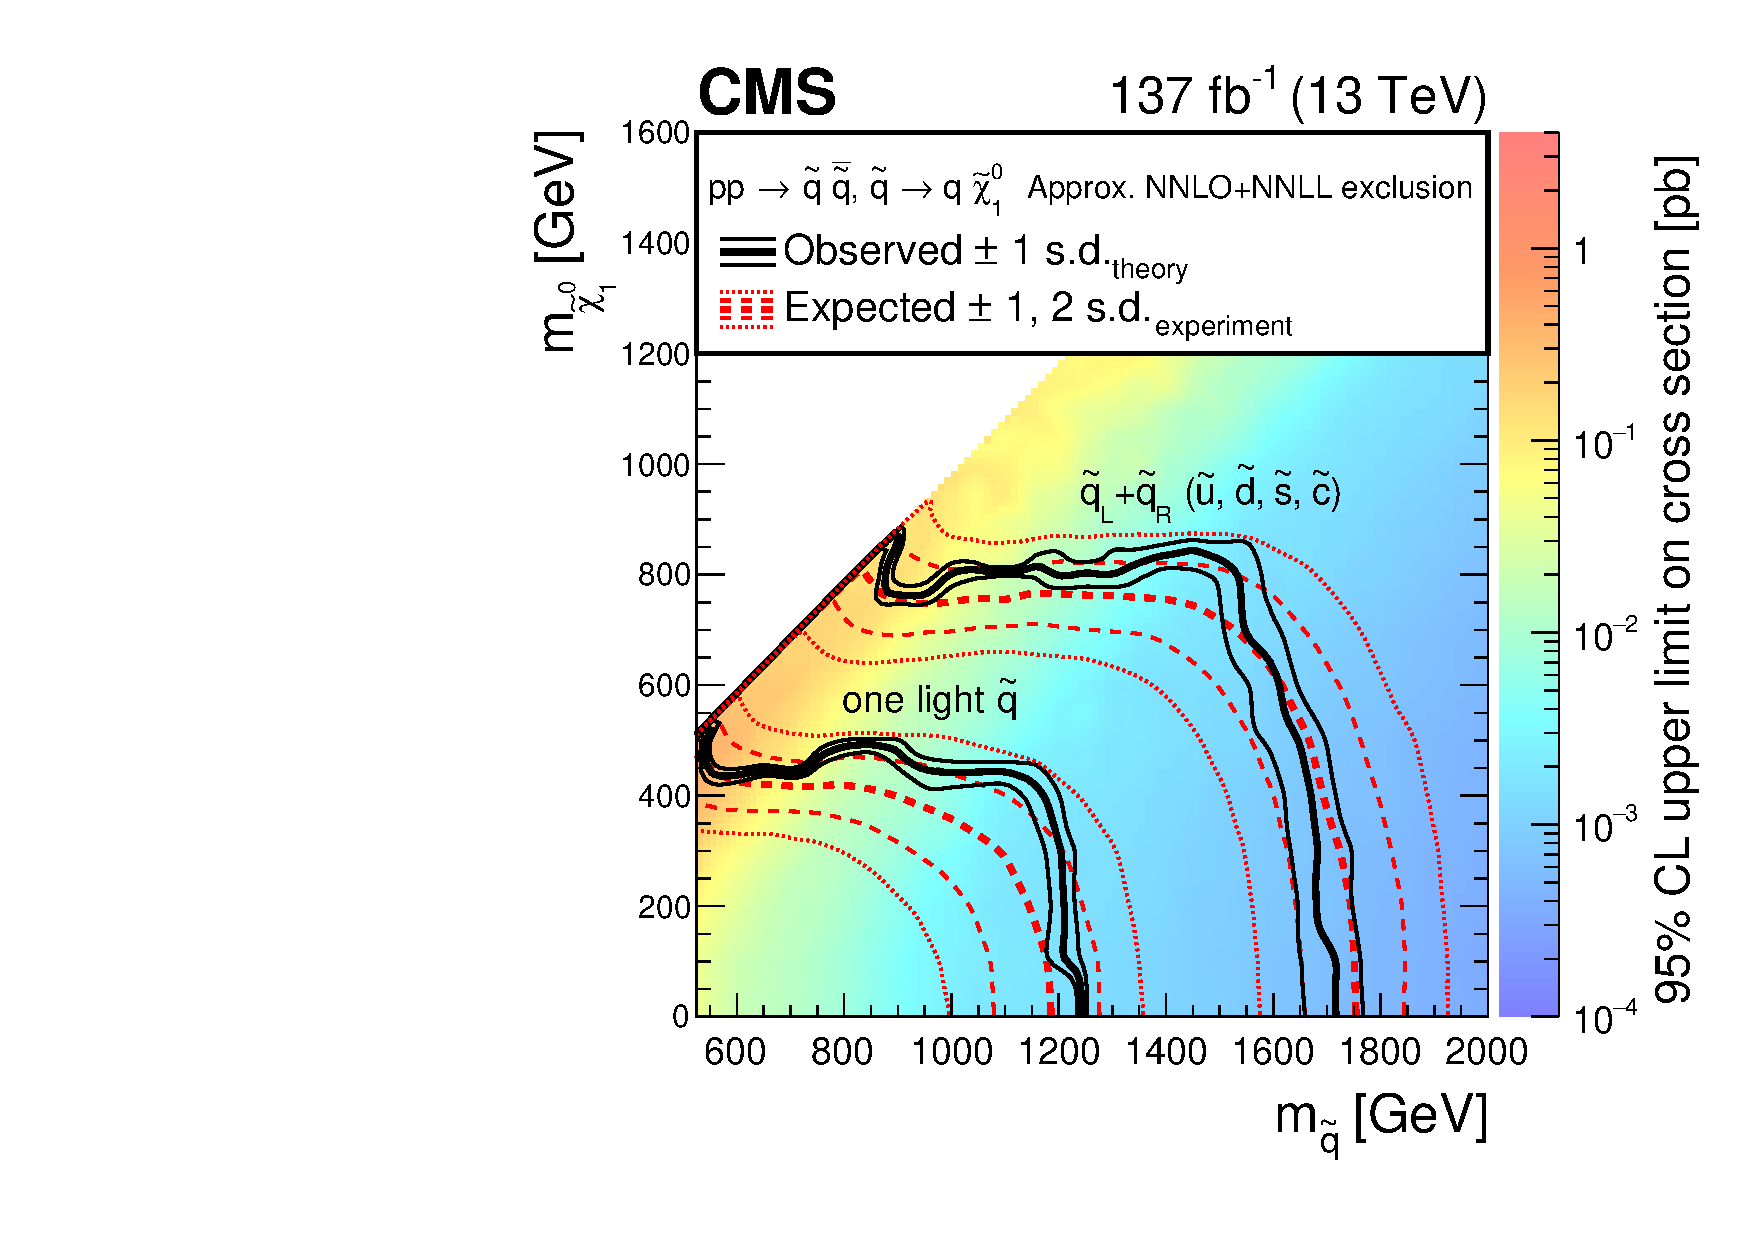
\includegraphics[width=0.48\textwidth]{figures/MT2_2019/Figure_013-a}
    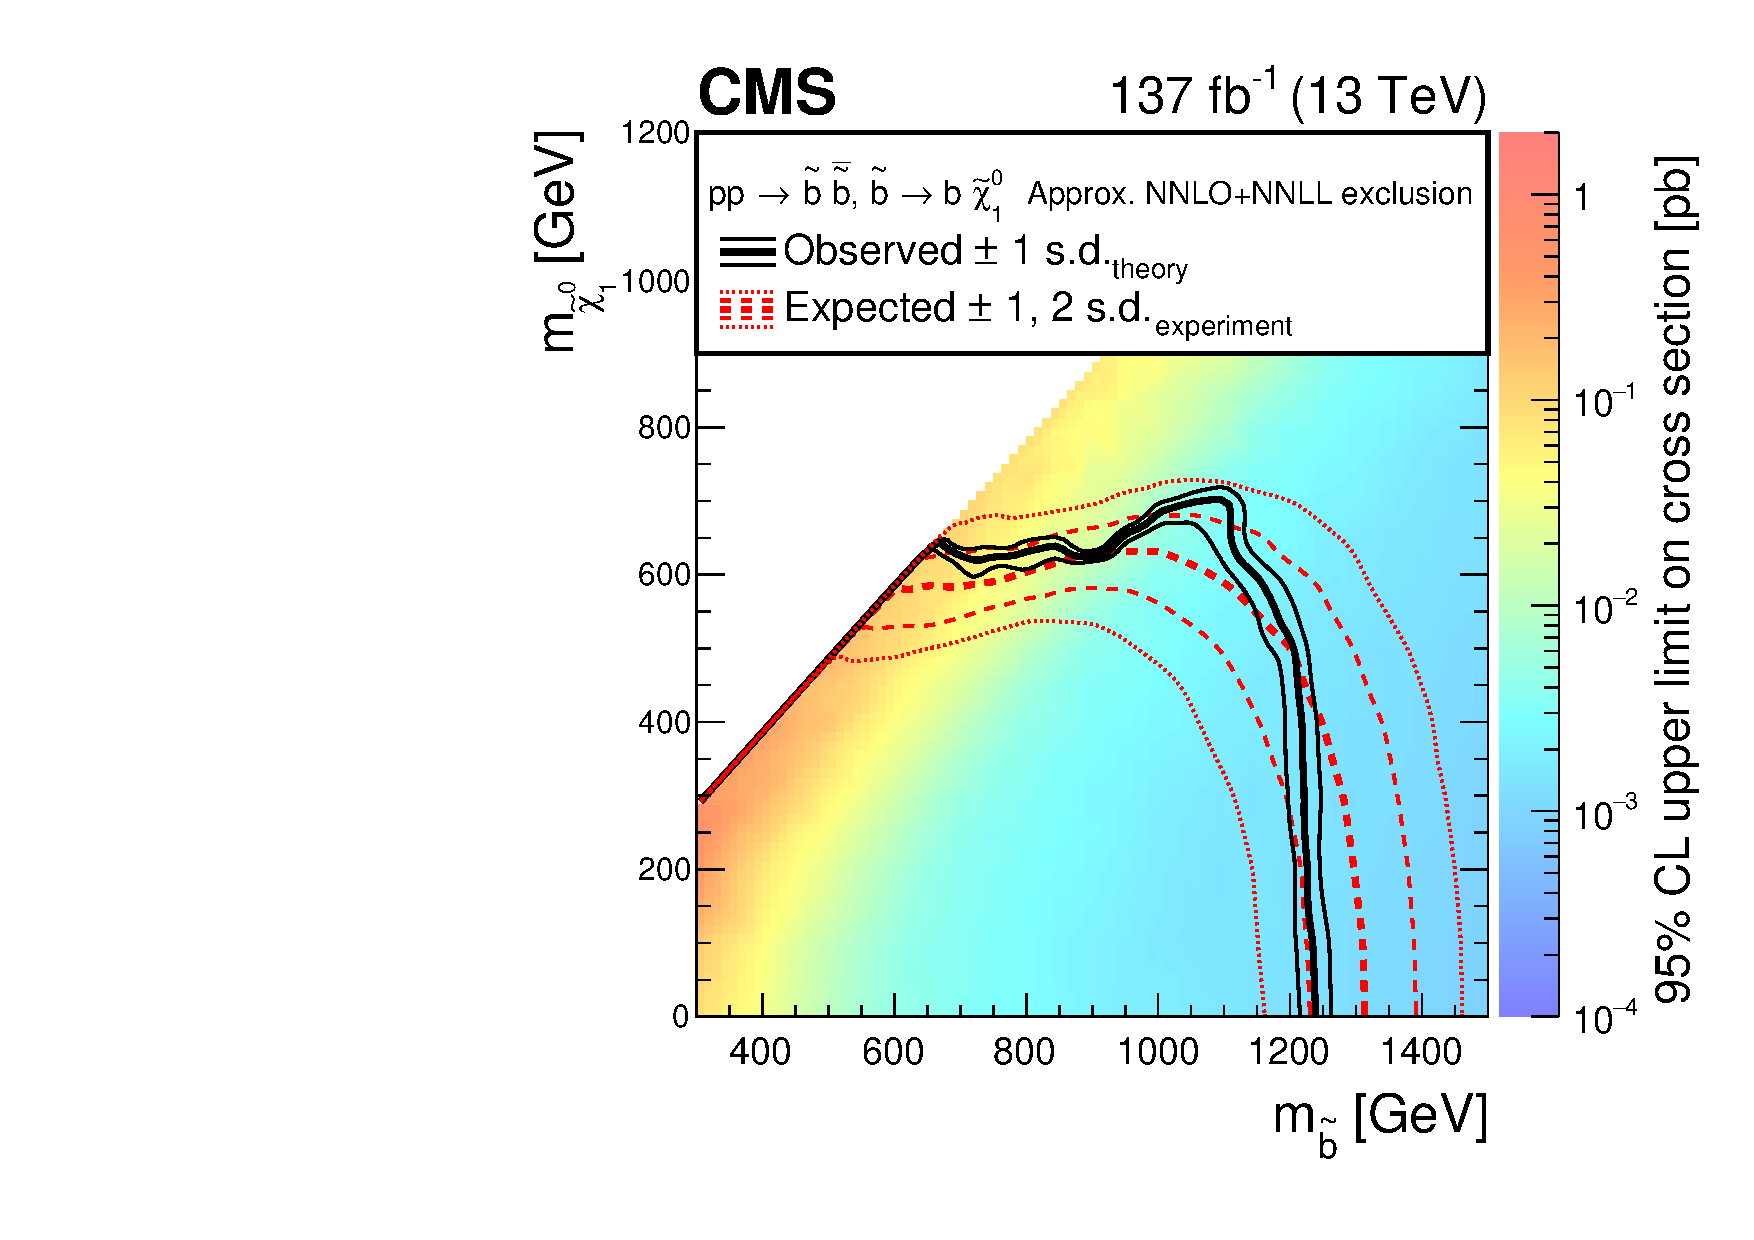
\includegraphics[width=0.48\textwidth]{figures/MT2_2019/Figure_013-b}
    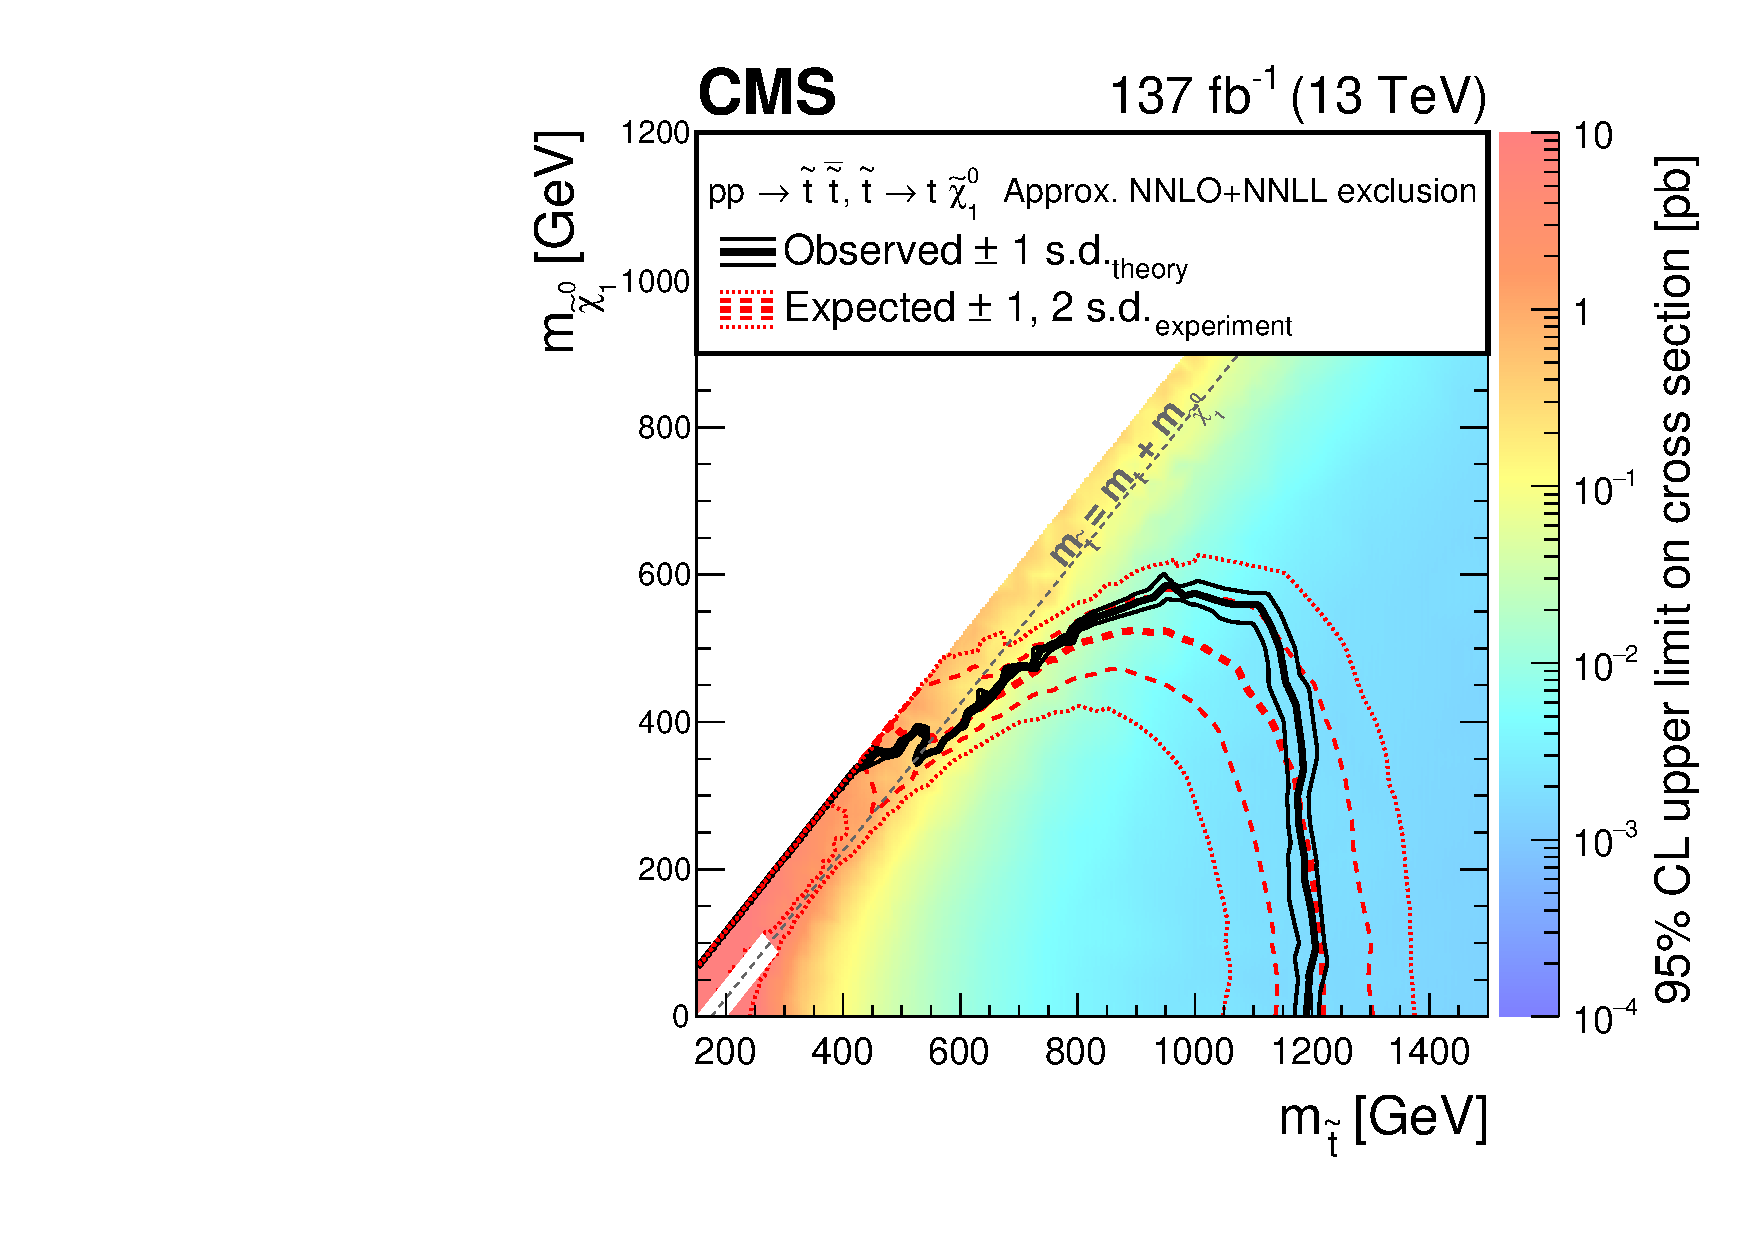
\includegraphics[width=0.48\textwidth]{figures/MT2_2019/Figure_013-c}
    \caption[Exclusion limit at 95\% \CL for (upper left) light-flavor squark pair production, (upper right) bottom squark pair production,
    and (lower) top squark pair production.]{Exclusion limit at 95\% \CL for (upper left) light-flavor squark pair production, (upper right) bottom squark pair production,
    and (lower) top squark pair production. Taken from \cite{MT2_2019}.}
    \label{fig:t2x}
\end{figure*}

\begin{figure*}[htbp!]
 \centering
   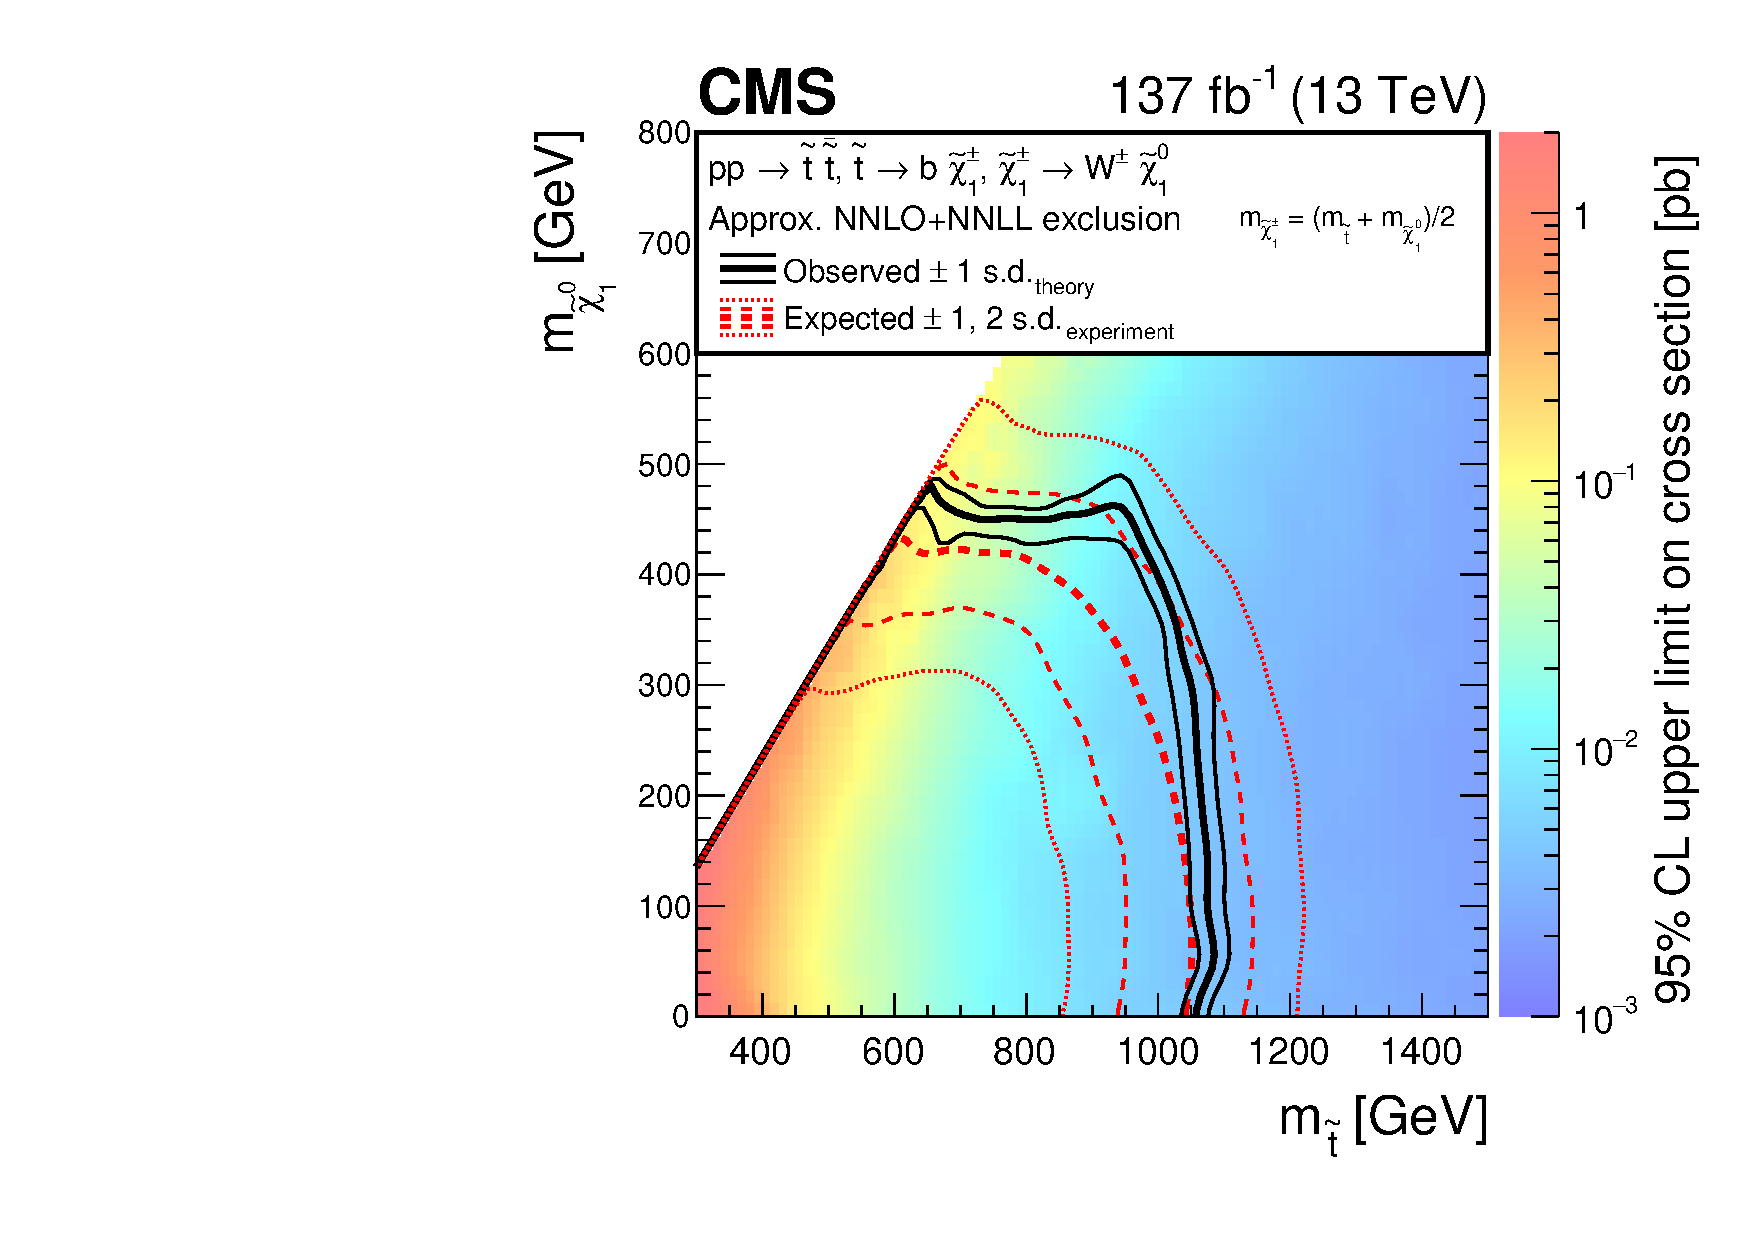
\includegraphics[width=0.49\textwidth]{figures/MT2_2019/Figure_014-a}
   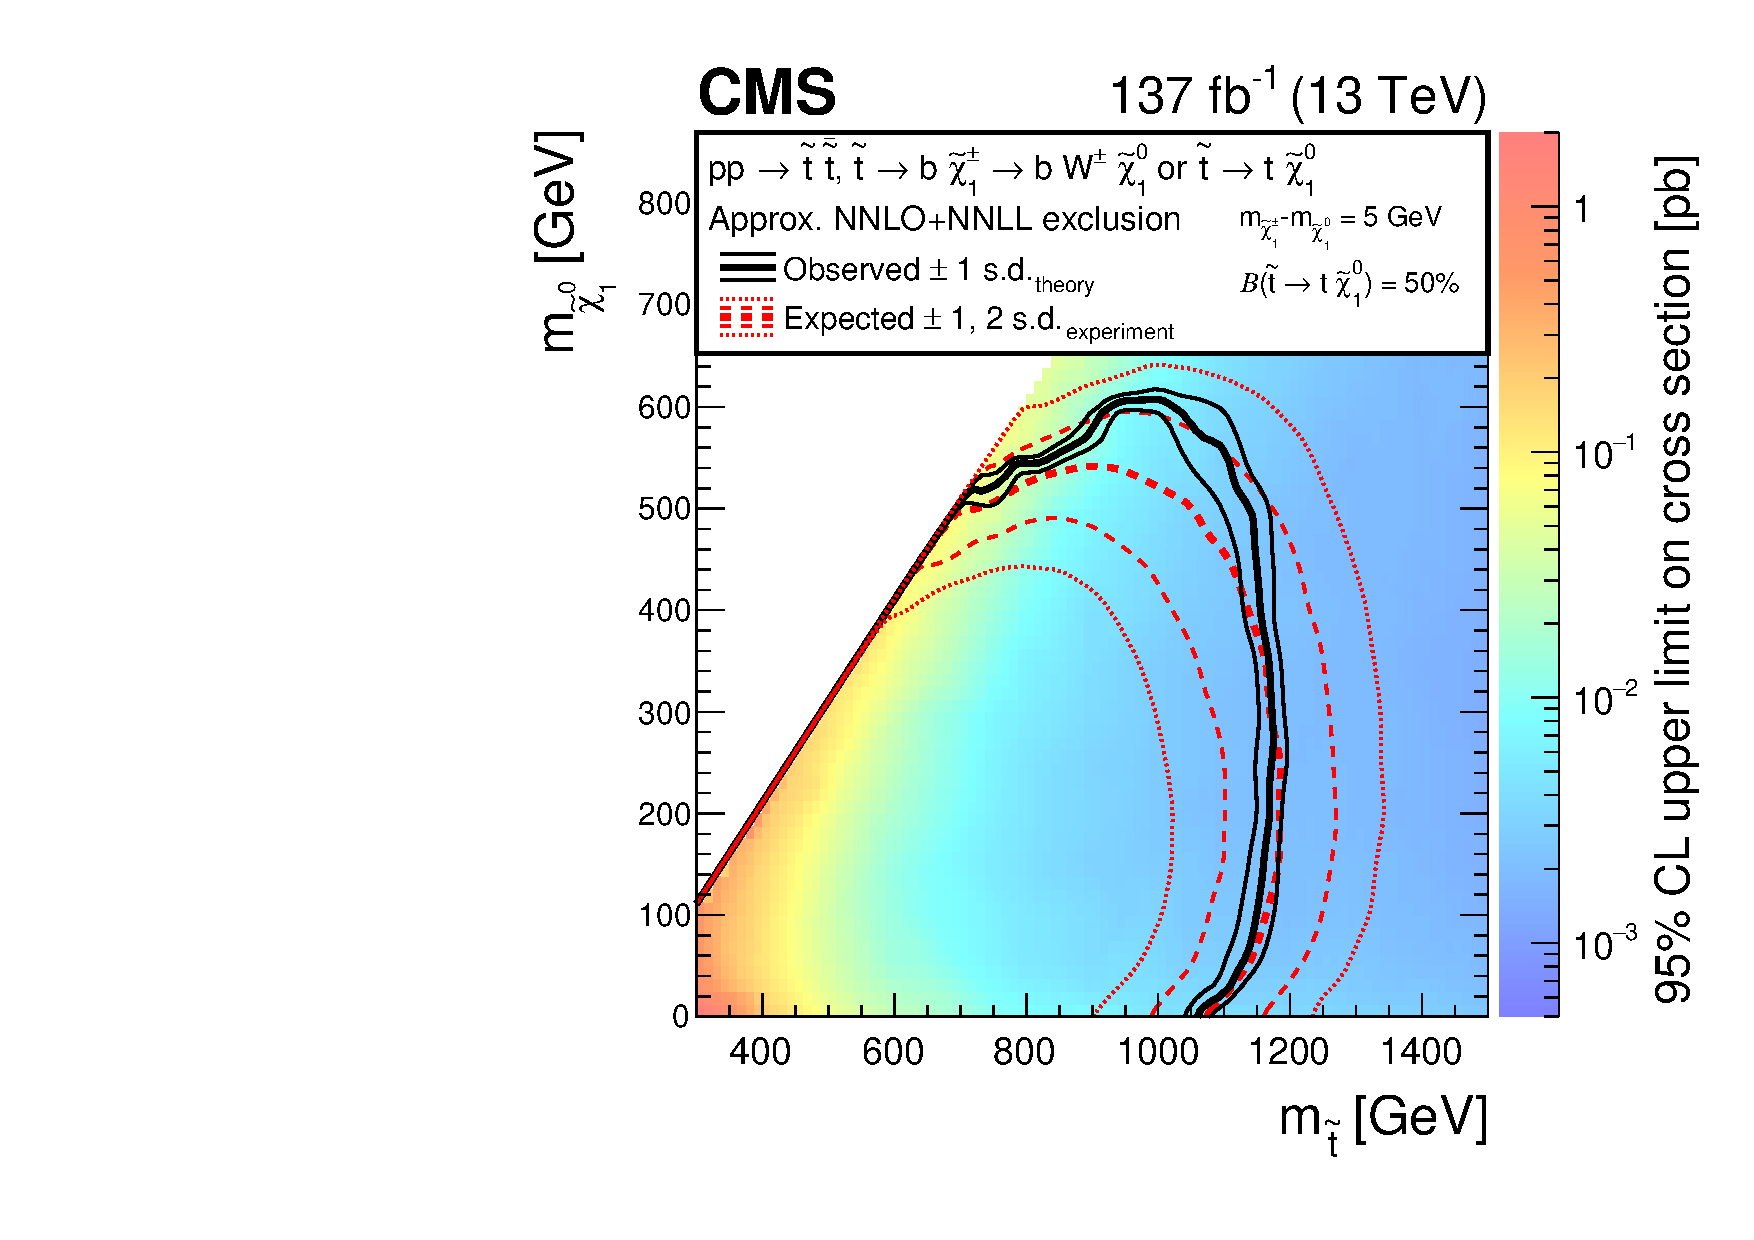
\includegraphics[width=0.49\textwidth]{figures/MT2_2019/Figure_014-b}
   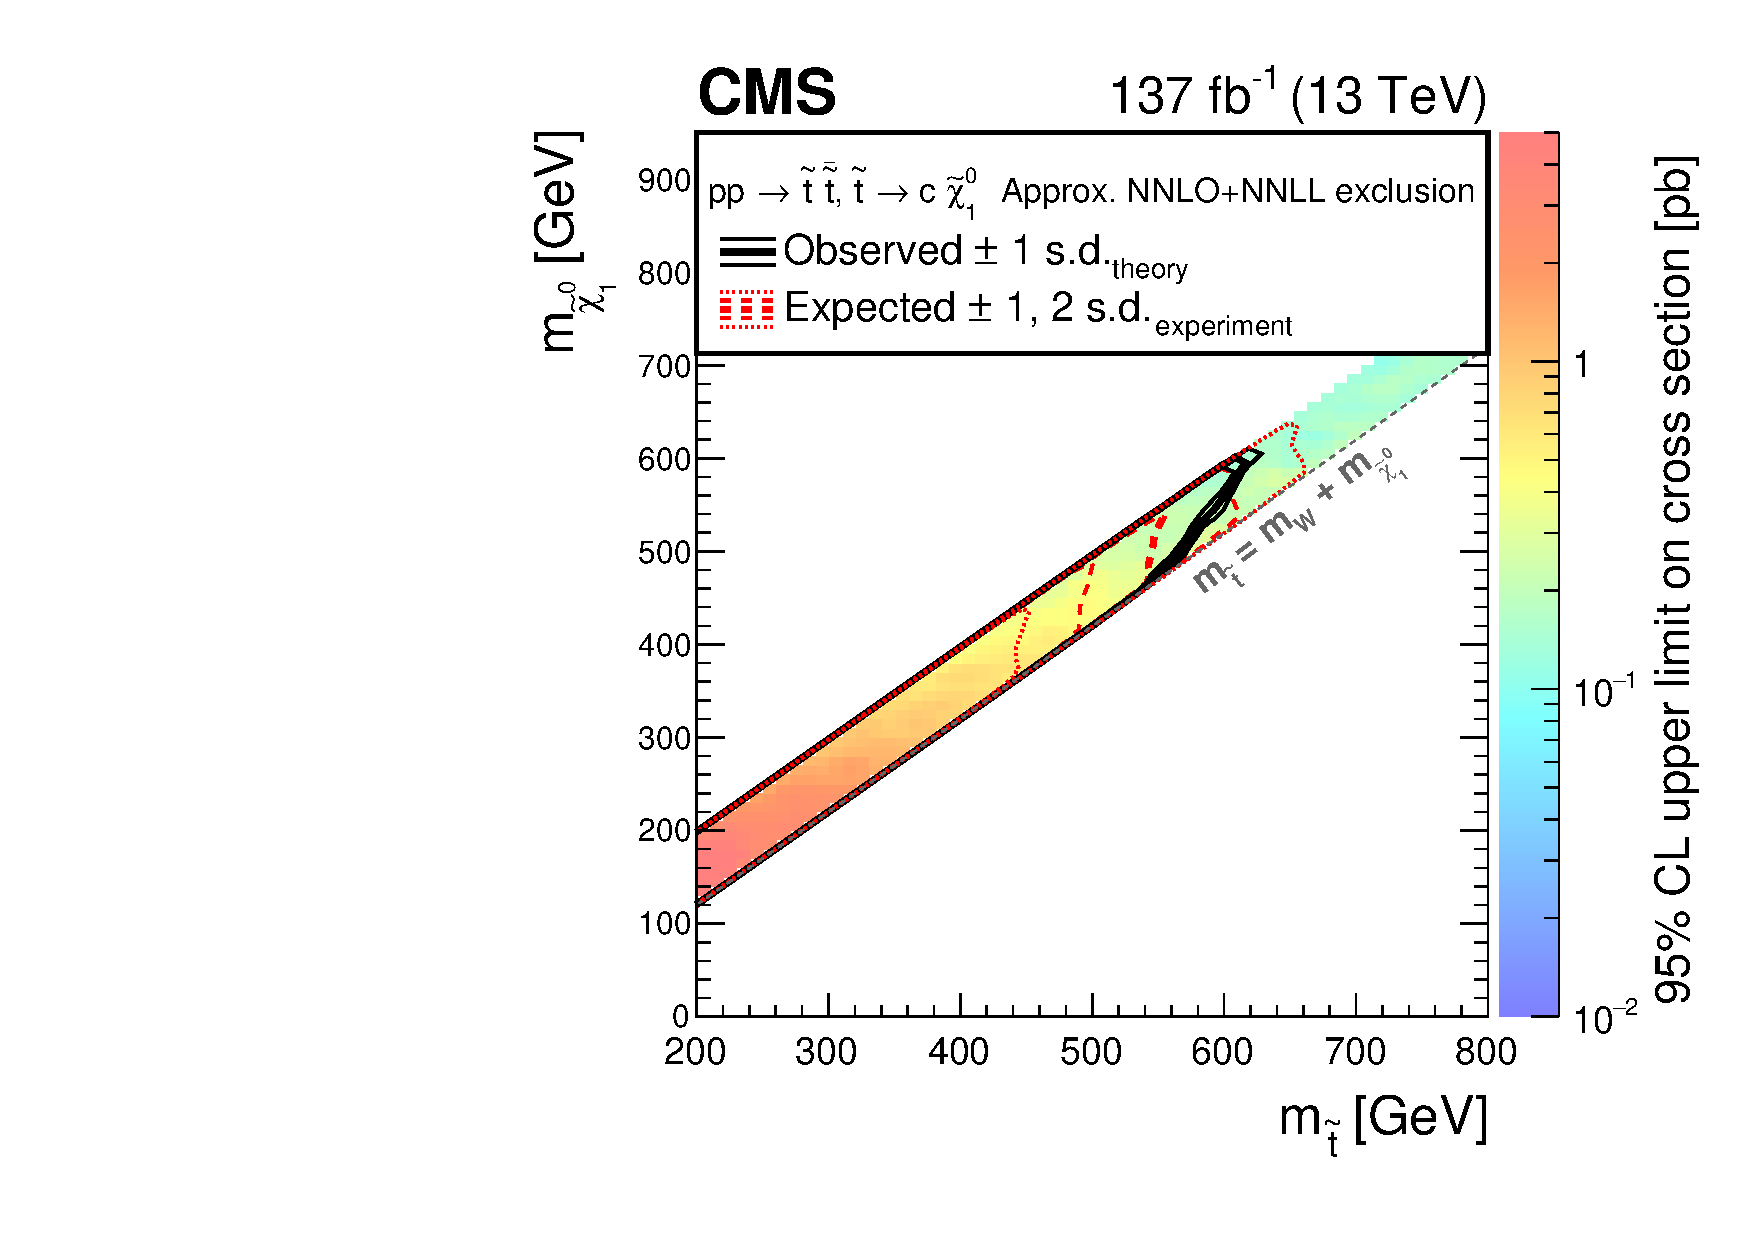
\includegraphics[width=0.49\textwidth]{figures/MT2_2019/Figure_014-c}
   \caption[Exclusion limit at 95\% \CL for top squark pair production for various decay modes of the top squark.]{
     Exclusion limits at 95\% \CL for top squark pair production and decay to (upper left) a bottom quark and \chargino, which subsequently decays to a W boson and \lsp, (upper right) either a bottom quark and \chargino or top quark and \lsp, or (lower) a charm quark and \lsp. Taken from \cite{MT2_2019}.}
   \label{fig:stop_other}
\end{figure*}

\begin{figure}[htbp]
 \centering
   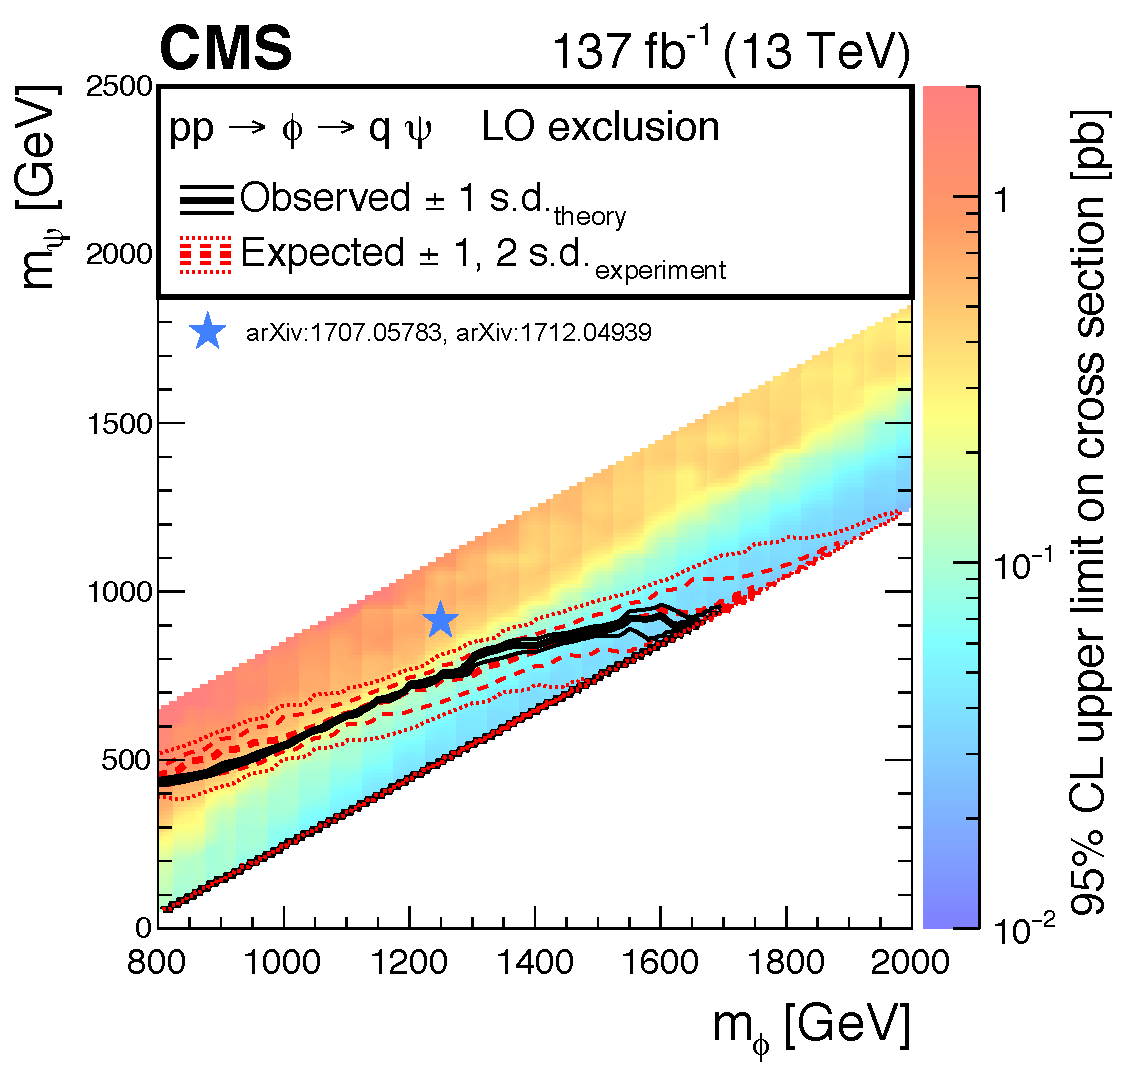
\includegraphics[width=0.49\textwidth]{figures/MT2_2019/Figure_015}
   \caption[Exclusion limit at 95\% \CL for the mono-$\phi$ model.]{
     Exclusion limit at 95\% \CL for the mono-$\phi$ model. 
     Only the portion of the mass plane of phenomenological interest was simulated.
     The star indicates the original authors' proposed best fit mass point, which remains unexcluded.
     Taken from \cite{MT2_2019}.}
   \label{fig:monophilimits}
\end{figure}

\begin{figure*}[htbp]
 \centering
   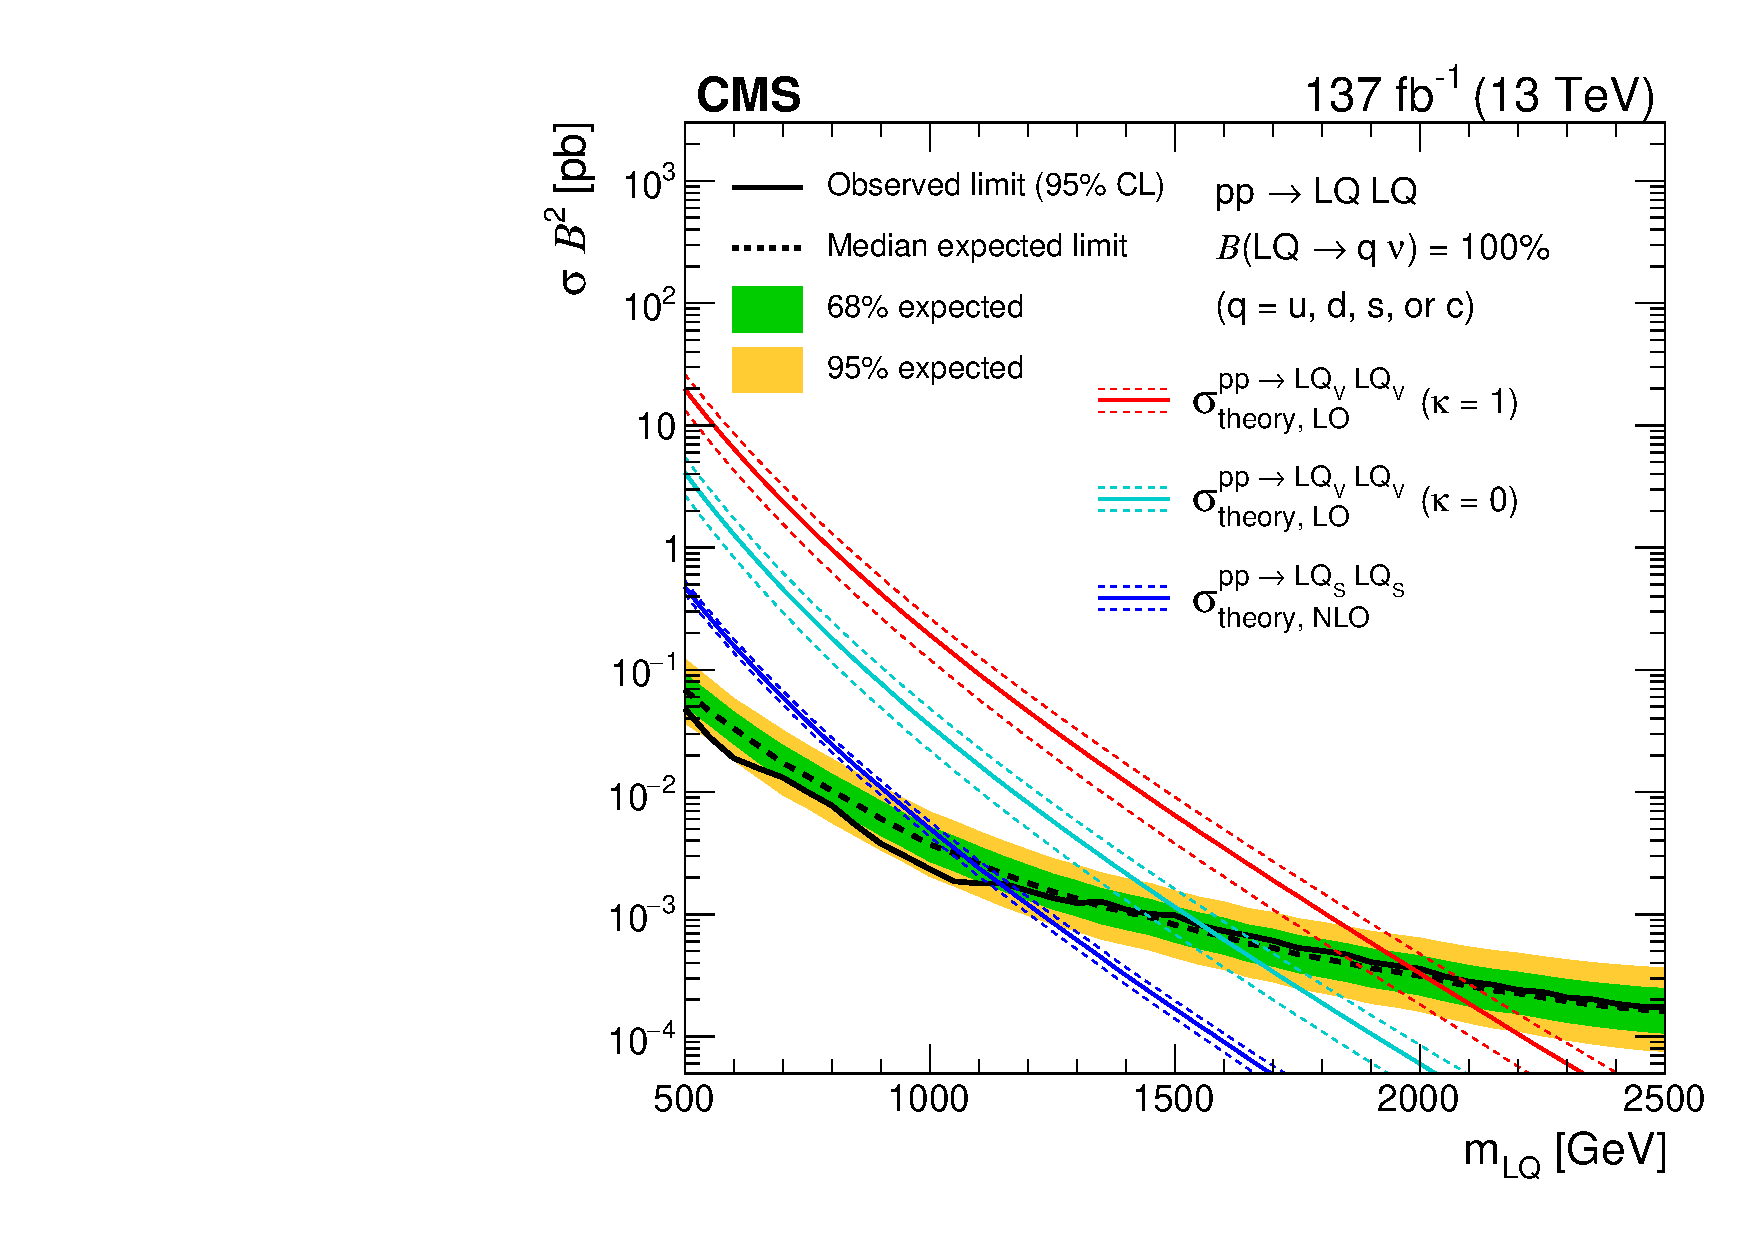
\includegraphics[width=0.49\textwidth]{figures/MT2_2019/Figure_016-a}
   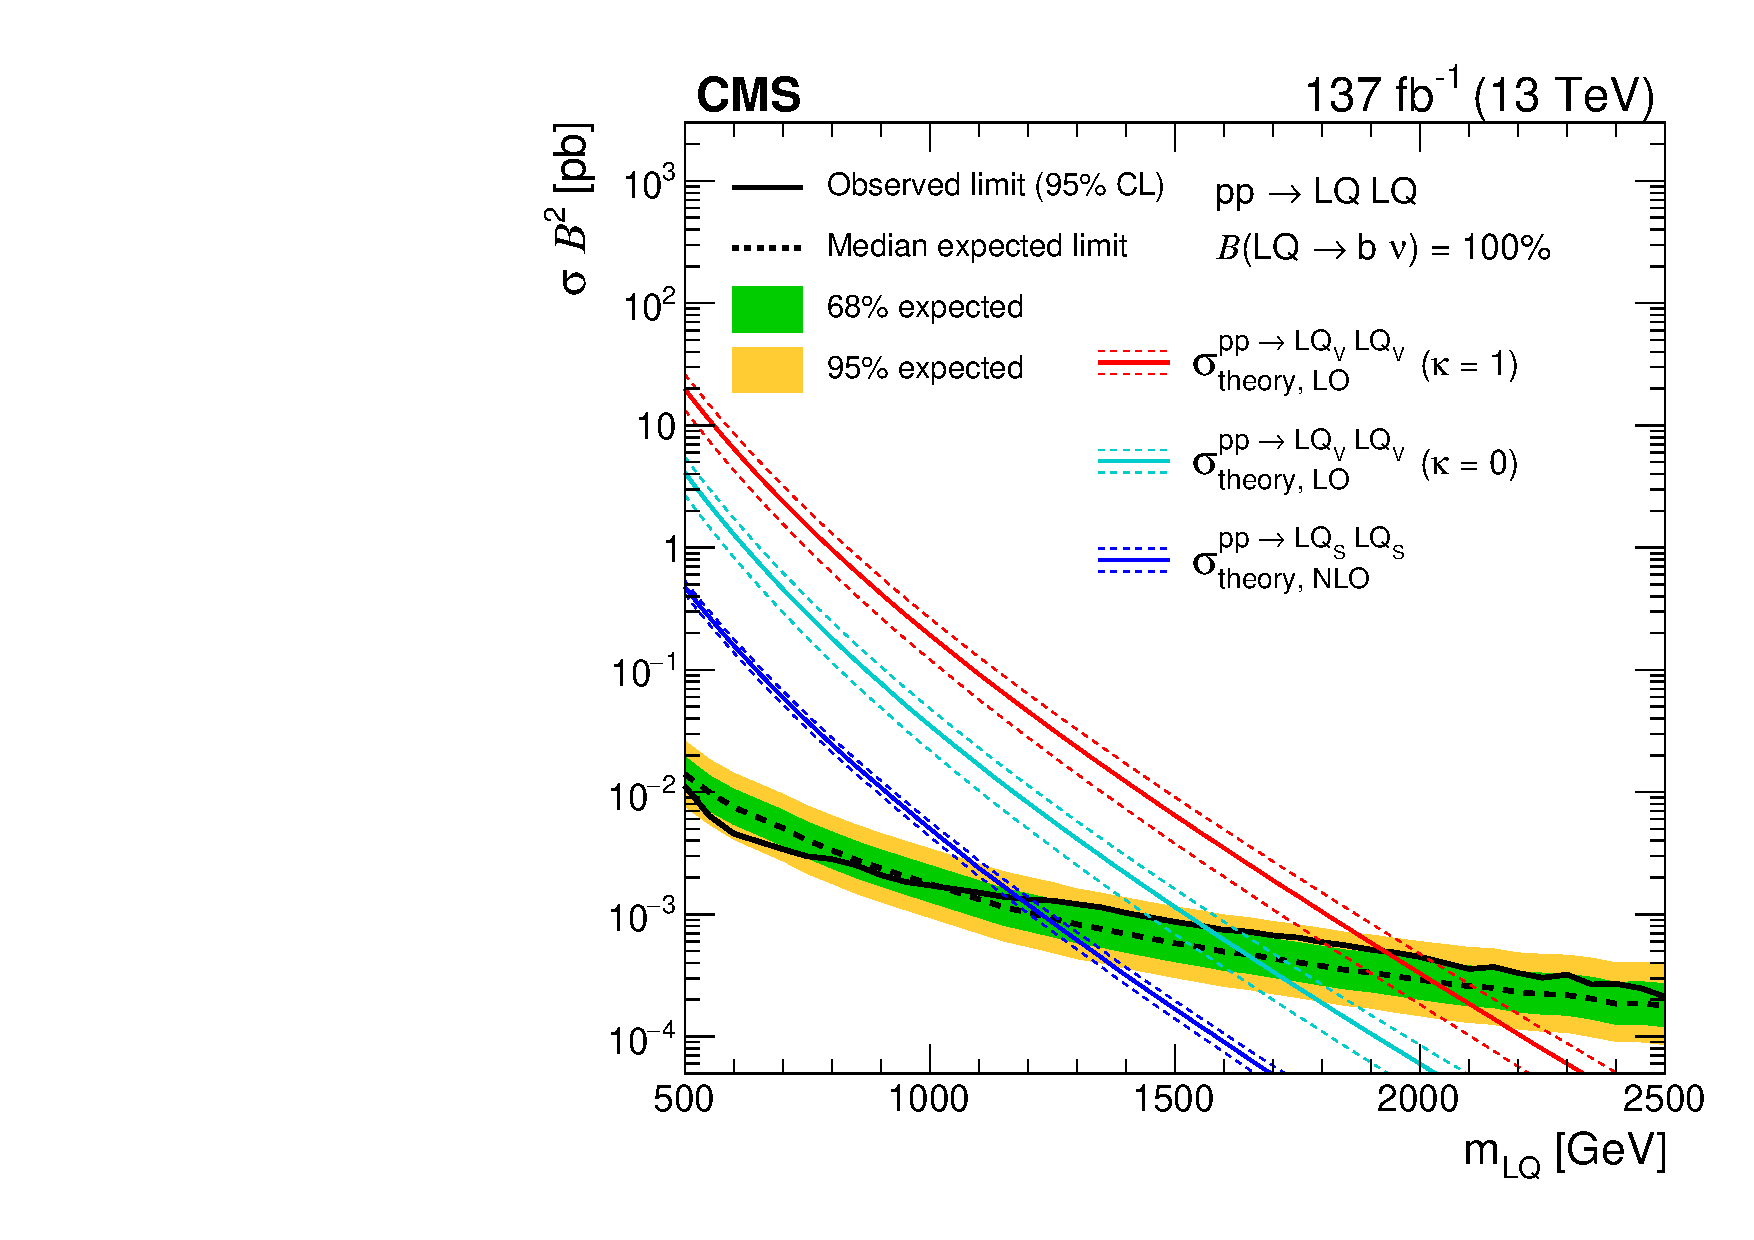
\includegraphics[width=0.49\textwidth]{figures/MT2_2019/Figure_016-b}
   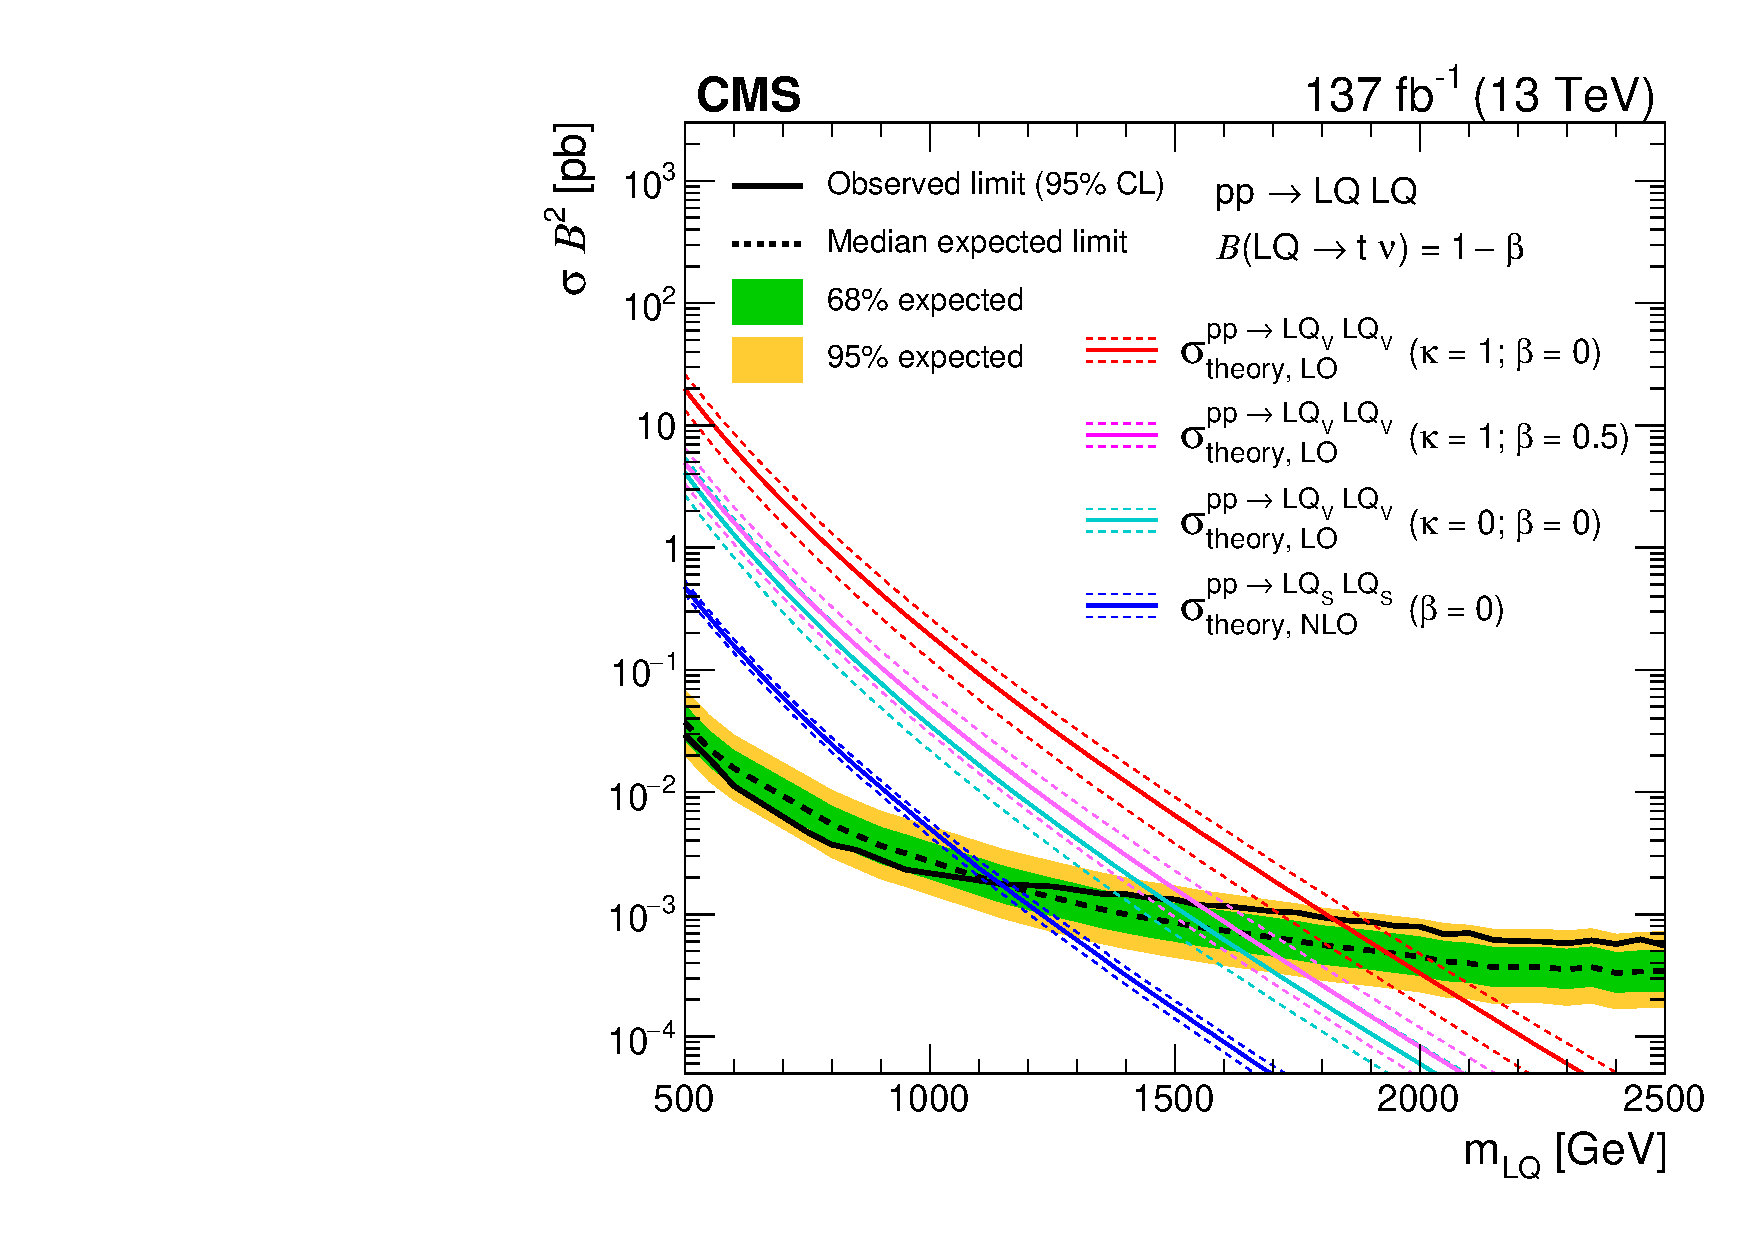
\includegraphics[width=0.49\textwidth]{figures/MT2_2019/Figure_016-c}
   \caption[Upper limits at 95\% \CL on the leptoquark production cross sections as a function of leptoquark mass.]{
     Upper limits at 95\% \CL on the leptoquark production cross sections as a function of leptoquark mass. 
     Unlike the limits on supersymmetric models, in which the mass of \lsp is a free parameter, the limits on leptoquarks are 1-dimensional in the leptoquark mass since the neutrino masses are known to be approximately zero.
     Taken from \cite{MT2_2019}.}
   \label{fig:lqlimit}
\end{figure*}

  Figure~\ref{fig:t5x} shows the exclusion curves for gluino pair production and decay to light quarks (upper), light quarks and the Z boson (lower left), and light quarks and the W boson (lower right).
  Figure~\ref{fig:t1x} shows the exclusion curves for gluino pair production and decay to bottom (left) and top (right) quarks.

  Figure~\ref{fig:t2x} shows the exclusion curves for light-flavor squark (upper left), bottom squark (upper right), and (lower) top squark pair production in which the top squark decays to a top quark. 
  The light-flavor figure contains two curves, one which assumes that there is only a single low mass light flavor squark, and another that assumes that there are eight light flavor squarks of (approximately) degenerate mass, which implies a production cross section eight times larger.
  The other top squark decay modes, in which the top decays to (upper left) a bottom quark and \chargino, which subsequently decays to a W boson and \lsp, (lower) a charm and \lsp, and (upper right) either \chargino and a bottom quark or \lsp and a top quark, are shown in Figure~\ref{fig:stop_other}.
  The charm decay channel is only shown for signal models with small mass splittings, as the top squark would strictly prefer to decay to a top quark and \lsp than to a charm quark and \lsp if kinematically allowed.

  Figure~\ref{fig:monophilimits} shows limits placed on the mono-$\phi$ model.
  Here, the horizontal axis is the mass of the singly-produced scalar $\phi$, and the vertical axis the mass of the invisible fermion $\psi$.
  A star indicates the mass point proposed by the original authors in \cite{monophi} as most phenomenologically interesting, which is not yet excluded.
  It is worth emphasizing that the background model is nevertheless consistent with data; this signal is simply very difficult to exclude with the \mttwo analysis methodology.
  To save computing resources, the mono-$\phi$ model is only simulated in the phenomenologically interesting subset of the mass plane, similarly to the top squark to charm model in Figure~\ref{fig:stop_other} (lower), hence the large white space beneath the considered range of masses.

  Figure~\ref{fig:lqlimit} shows limits for leptoquarks decaying to (upper left) a light flavor quark and neutrino, (upper right) a bottom quark and neutrino, and (lower) a top quark and neutrino.
  As the mass of the neutrinos, in contrast to the mass of \lsp, are known to be approximately zero, the leptoquark limits are one dimensional, in the leptoquark masses.

  The limits produced by this edition of the classic search improve upon the limits set by the previous edition \cite{MT2_2016} by hundreds of GeV, and in most cases are the strongest constraints on their respective signal models yet produced by any experiment.

  \subsection{Future of the Classic \mttwo Search} \label{sec:MT2future}

  The current limits produced by the classic \mttwo search are impressive, and are unlikely to improve much in the near future.
  The pair production cross section for squarks and gluinos drops rapidly with mass, as shown in Figure~\ref{fig:SUSYxsec}.
  Generically, a factor of 10 improvement in sensitivity is necessary to push the exclusion limits outward by around 500 GeV along the horizontal axis.
  At this mature statistical stage, a factor of 10 improvement in sensitivity requires a factor of 100 increase in the integrated luminosity, infeasible in the near future.
  Improvement along the \lsp axis is similarly difficult due to large backgrounds and low signal efficiency for models with small mass splittings.
  Therefore, attention in the near future will turn to other new techniques, one of which is discussed in the next section.

\section{Disappearing Tracks Search} \label{sec:distracks}

  \subsection{General Description} \label{sec:distracksdescription}

  As searches like that discussed in the previous section approach the practical limits of their sensitivities at the LHC, interest has grown in targeting plausible signals with peculiar features that more standard searches do not exploit.
  Among these features are those produced by relatively long-lived particles (LLPs) that do not decay promptly at the collision point, but instead travel a macroscopic distance into the detector before decaying. 
  An overview of some possibilities in the context of supersymmetry is provided in \cite{LLPsAtLHC}.

  One of these signatures is a disappearing track, produced when a charged particle, such as \chargino, travels into the tracker, then decays to an invisible particle, such as \lsp, with a mass so nearly equal to that of the decaying charged particle that the visible products of the decay are too low energy to be reconstructed. 
  The supersymmetric parameter space is vast and there is no way to know which if any version of supersymmetry is realized in nature, but models including LLPs that would produce disappearing tracks at CMS have been argued to be especially plausible on theoretical grounds \cite{distracks1, distracksAMSB, AMSBlifetime}.
  The \mttwo analysis is already well-optimized for all-hadronic supersymmetry, so it is natural to search for all-hadronic decays of these models by extending it with a disappearing track search.
  This extension begins with exactly the same set of selected events as the classic search, and then further selects the subset of events possessing a disappearing track.

  \subsection{Challenges} \label{sec:distrackschallenges}

  The disappearing tracks search must confront a pair of significant challenges.

  First, the background (see Section~\ref{sec:distracksbg}) entirely consists of events in which reconstruction failed, analogous to the classic search's detector mismeasurement background that was discussed in Section~\ref{sec:MT2QCD}, and is difficult to understand and estimate for many of the same reasons.
  Simulation cannot be trusted to account for all of the detector details that lead to extremely rare reconstruction errors.
  While the classic search can mitigate the impact of this issue with selections that make the mismeasurement background subdominant compared to the better understood neutrino backgrounds, this is not possible for the disappearing track search since no such genuine background exists.
  Moreover, since the background is dependent on details of the detector, it is strongly affected when these details change.
  Most prominently, the CMS pixel detector was entirely replaced between the 2016 and 2017 data taking periods \cite{phase1}, and this profoundly affected CMS track reconstruction, to the extent that the disappearing track search must treat the 2016 data entirely separately from the 2017 and 2018 data.
  The detector's state also evolves more subtly over the data taking period, due in large part to inevitable radiation damage, and the analysis must track, study, and account for the effect of this evolution on the occurrence of disappearing tracks.
  
  Second, disappearing tracks are extremely rare.
  This is of course one of the motivations for the disappearing tracks extension---they are a powerful tool to discriminate between background and likely signal events---but it also makes them difficult to study.
  
  Nevertheless, the disappearing tracks search produced a data-driven background estimation procedure, described in Section~\ref{sec:distracksbgest}, that was successfully validated in data, and achieved the best sensitivity to disappearing tracks in supersymmetric models to date.
  
  \subsection{Signal Models} \label{sec:distrackssig}

  \begin{figure*}[htbp]
    \centering
    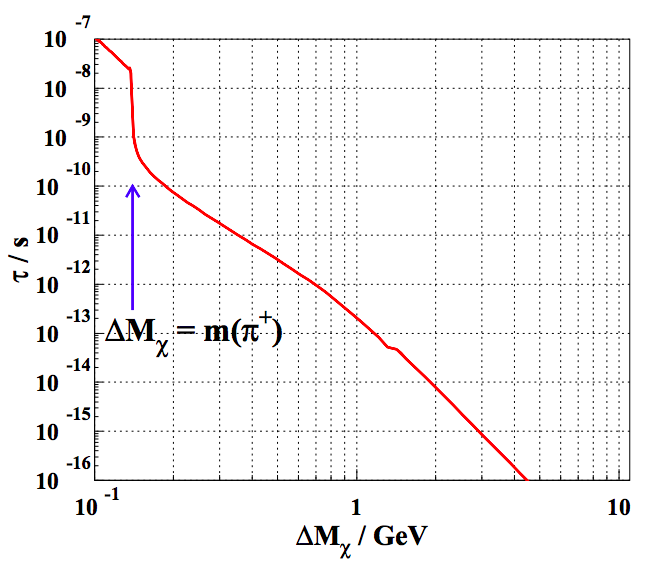
\includegraphics[width=0.55\textwidth]{figures/chargino_lifetime.png}
    \caption[Lifetime of \chargino as a function of mass splitting.]{
      The rest frame lifetime of \chargino as a function of the \chargino-\lsp mass splitting. 
      The lifetime is macroscopic for mass splittings less than 1~GeV in a broad class of supersymmetric models, a regime that is realized  when the superpartner mass scale is much larger than the Standard Model mass scale. 
      This mass splitting is so small that the charged daughter of \chargino decay is too low energy for track reconstruction.
      Thus, \chargino lives long enough to produce a short track in the CMS tracker, then disappears when it decays to \lsp and a lost charged daughter.
      For mass splittings less than $M_{\pi} \approx 140$~MeV, indicated on the plot, the lifetime of \chargino is so long that it typically does not decay inside the tracker.
      As a result, the sweet spot for the disappearing tracks search is lifetimes on the order of hundreds of MeV.
      The discontinuity at a mass splitting of 1.4~GeV is not physical.
      Taken from \cite{AMSBlifetime}.}
    \label{fig:charginolifetime}
  \end{figure*}

  For the class of supersymmetric models discussed in \cite{distracksAMSB} \& \cite{AMSBlifetime}, the relative mass splitting of \chargino and \lsp is proportional to $(M_{W}/\mu)^4$, where $\mu$ is a parameter that roughly represents the energy scale of supersymmetry.
  Non-observation of superpartners thus far at the LHC suggests that $\mu$ is probably large, on the order of TeV, implying $(M_{W}/\mu)^4 < 10^{-4}$.
  Such a tiny mass splitting leads to a remarkably long \chargino lifetime, shown in Figure~\ref{fig:charginolifetime}.

  \begin{figure*}[htbp]
    \centering
    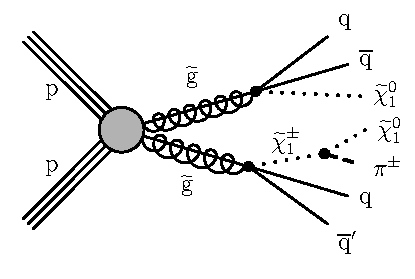
\includegraphics[width=0.3\textwidth]{figures/MT2_2019/Figure_010-a}
    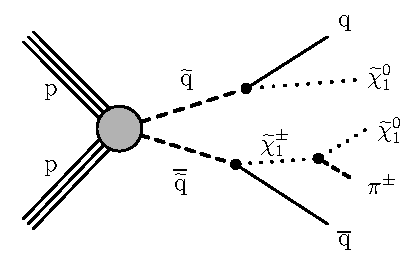
\includegraphics[width=0.3\textwidth]{figures/MT2_2019/Figure_010-b}
    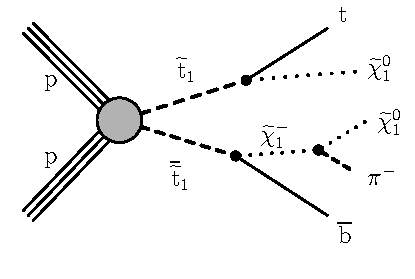
\includegraphics[width=0.3\textwidth]{figures/MT2_2019/Figure_010-c}
    \caption[Diagrams for (left) gluino, (center) light-flavor squark, and (right) top squark pair production, in which the gluinos and squarks can decay via a long-lived \chargino]{Diagrams for (left) gluino, (center) light-flavor squark, and (right) top squark pair production, in which the gluinos and squarks can decay via a long-lived \chargino. In this analysis, the gluino is taken to decay with branching fraction 1/3 each to the \lsp, \chargino plus, and \chargino minus. Squarks decay with branching fraction 1/2 each to the \lsp and the \chargino allowed by charge conservation. The \chargino mass is greater than the \lsp mass by hundreds of MeV, so that the charged product of the \chargino decay is too soft to be detected. Taken from \cite{MT2_2019}.}
    \label{fig:charginodiags}
  \end{figure*}
  
  Motivated by these models, the disappearing track seach considers signals that include an intermediate \chargino in the superpartner decay chain, similar to the models in Figure~\ref{fig:susyproduction} (upper right, lower left, and lower center) considered by the inclusive search.
  The \chargino is taken to be long-lived, only hundreds of MeV more massive than \lsp.
  Specifically, the rest frame \chargino lifetime, $\tau_0$, is varied from $c\tau_0 = 1$~cm to $c\tau_0 = 2000$~cm.
  This range of lifetimes is selected because the CMS tracker extends from $r\approx10$~cm to $r\approx 100$~cm, and a significant fraction of \chargino decays must occur inside the tracker for the disappearing track search to have meaningful sensitivity.
  If the decay occurs outside the tracker, the track does not disappear.
  The full set of models considered is shown in Figure~\ref{fig:charginodiags}.
  
  In the model at left, gluinos are pair-produced and decay with equal probability either to \chip, \chim, or \lsp, and light-flavor quarks.

  In the center second, light flavor squarks are pair-produced and decay with equal probability either to the allowed charge of \chargino, or to \lsp, and a light-flavor quark.

  In the model at right, top squarks are pair-produced and decay with equal probability either to the allowed charge of \chargino, or to \lsp, and a bottom quark.

  \begin{figure}[h!]
    \centering
    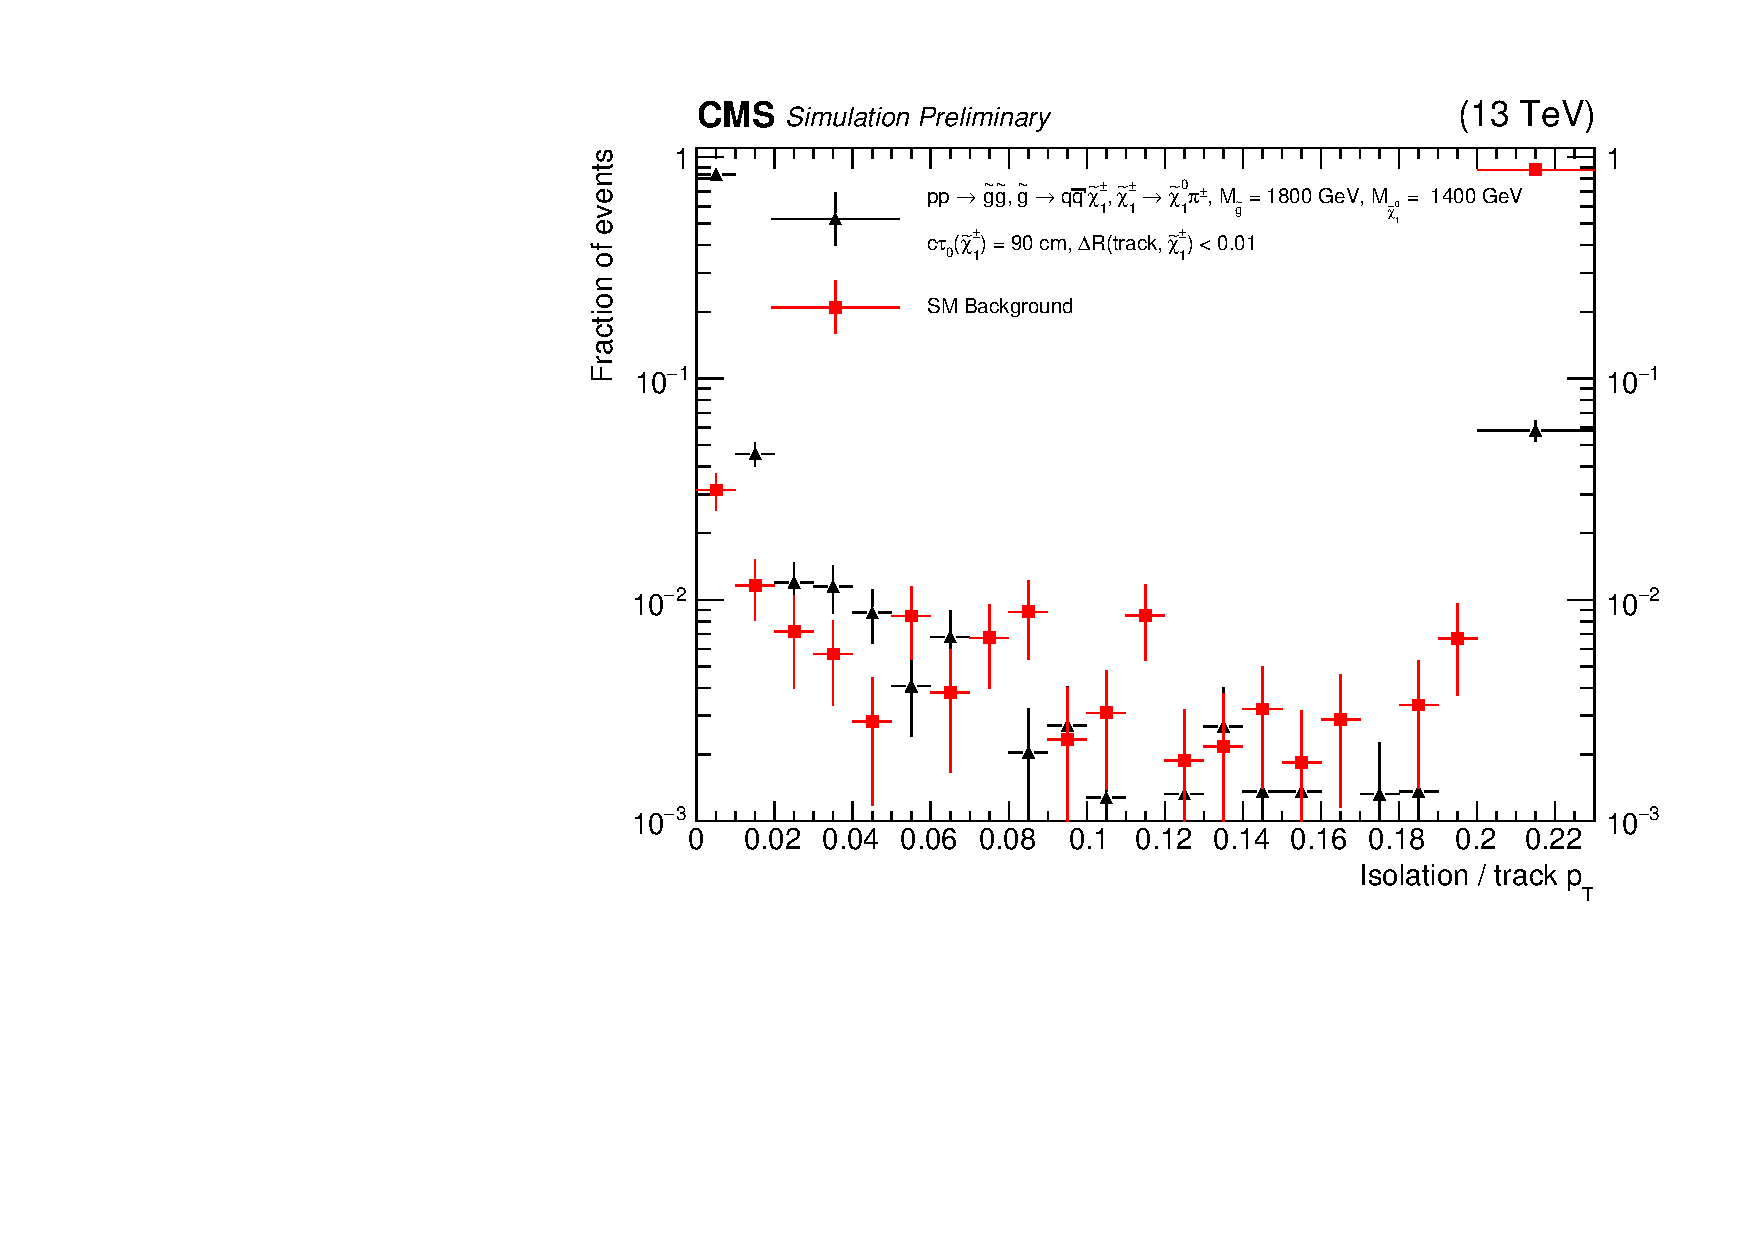
\includegraphics[width=0.85\textwidth]{figures/reliso_SvsB.pdf}
    \caption[Comparison of signal and background Short Track relative isolation distributions.]
            {Disappearing tracks produced by \chargino decays (black triangles) tend to be much more isolated than disappearing tracks in background events (red squares).
              All selections listed in Table~\ref{tab:shorttrackselection} are applied except the isolation selections.
              The last bin is an overflow bin, containing every track failing the relative isolation selection.
              The events containing those tracks will either populate control regions, or be rejected entirely, as described in Section~\ref{sec:distracksbgest}.
              Additional material from \cite{MT2_2019}.}
            \label{fig:distracksisolation}
  \end{figure}  

  The disappearing tracks produced by \chargino decays tend to be very high quality and highly isolated (shown in comparison with background in Figure~\ref{fig:distracksisolation}), with negligible energy deposits in any of the calorimeter cells along the track's extrapolated path.
  The quality metrics in this context include the track's impact parameter with respect to the primary vertex, the size of the uncertainty in the track's assigned \pt, and the number of tracker layers in which the track failed to leave a hit when one would be expected.
  Alongside isolation, shown in Figure~\ref{fig:distracksisolation}, these quality metrics allow for signal-like disappearing tracks to be distinguished from disappearing tracks that are very likely to be due to a reconstruction error.
  This forms the basis of the background estimate described in Section~\ref{sec:distracksbgest}.

  \subsection{Backgrounds} \label{sec:distracksbg}

  In contrast to the classic search, there are no irreducible disappearing track backgrounds produced by the Standard Model.
  However, there are a number of detector reconstruction issues that can lead to apparent disappearing tracks, many of which can be greatly or even entirely rejected by various cleaning selections.

  Of the near-entirely reducible backgrounds, the largest before cleaning is that produced by electrons undergoing unusually strong bremsstrahlung inside the tracker, effectively converting the electron into a photon.
  While electrons are charged and therefore produce tracks, photons are neutral and do not.
  So, these tracks disappear, but can normally be rejected due to large photon energy deposits in the electromagnetic calorimeter cells to which the track extrapolates.
  However, some ECAL cells do not perform well for a variety of reasons and may fail to register the photon energy deposits, and so fail to veto the disappearing track.
  Fortunately, the majority of the ECAL performs well enough to make this background significant only for tracks extrapolating to defective cells.

  Defective cells are mapped and vetoed using a tag-and-probe strategy, in which a PF electron ``tag'' identifies potential $Z\rightarrow e^+e^-$ events, and a disappearing track of opposite charge serves as the ``probe.''
  If an event contains exactly one PF electron, the event is searched for a disappearing track of opposite charge, under the hypothesis that the event was in fact $Z\rightarrow e^+e^-$ and the second electron was not successfully reconstructed due to the conversion process described above.
  If such a track is found and the invariant mass of the electron-disappearing track pair is consistent with the mass of the Z boson, the region of the ECAL to which the disappearing track extrapolated is deemed faulty.
  $Z\rightarrow e^+e^-$ events are sufficiently common that the map of faulty ECAL cells can be assembled as a function of time.
  As expected, the performance of the ECAL steadily degrades over time, so that the fraction of the ECAL that must be vetoed increases from 2016 to 2017 to 2018.
  This veto essentially entirely rejects the electron conversion background, but at a price. 
  It is the single largest cause of signal inefficiency, as 15-20\% of signal disappearing tracks point, by chance, into vetoed regions of the ECAL.

  Another, much smaller reducible background is produced by the decay of strange baryons, including the $\Xi^{\pm}$, $\Sigma^{\pm}$, and $\Omega^{\pm}$.
  These baryons have lifetimes in the proper range to produce tracks 10s of centimeters long, before decaying with a small mass splitting to a neutral baryon and a charged daughter that is sometimes low enough \pt to escape reconstruction.
  While these tracks disappear from the perspective of the tracker and the ECAL, the neutral baryon is still detectable in the hadronic calorimeter via its nuclear interactions, which allows for efficient rejection of this background.
  Additionally, strange baryons are almost always found inside jets, so the vast majority of their tracks can be vetoed on the basis of isolation.
  Even so, a region of the HCAL with known performance issues in 2018 showed significantly increased disappearing track counts that required it to be vetoed, likely in part because of this background.

  The final two backgrounds are fake tracks and mesons, mostly pions, that undergo nuclear interactions in the tracker, neither of which can be entirely rejected.
  
  Fake tracks are tracks comprised of hits that are not all associated to the same genuine particle.
  The probability that track reconstruction produces a fake track is small, and can be suppressed by requiring that tracks pass a sophisticated selection called high purity, as shown in Figure~\ref{fig:trackfakerate} for the 2016 tracker \cite{cmstracking}, which improved after the pixel tracker upgrade between 2016 and 2017 \cite{cmstrackingphase1}.
  Furthermore, the probability that more than 3 or 4 unassociated hits will be strung together into a track is negligible, limiting the fake track background to very short tracks.
  It is also rare for unassociated hits to lie on a tight, relatively straight line; instead, they tend to be somewhat scattered.
  Therefore, fake tracks also tend to be have low assigned \pt, since low energy track have greater curvature in the detector's magnetic field.
  The disappearing tracks analysis considers only tracks with $\pt > 15$~GeV in part to avoid the majority of the fake track background.

  While the fake track background is limited to shorter tracks, the meson background is not and so constitutes the dominant longer disappearing track background.
  This background is generated when a meson undergoes a nuclear interaction inside the tracker, and showers in such a way that no single charged daughter is high enough energy to be reconstructed as a track, and any neutral products are sufficiently low energy or widely scattered that calorimeter deposits are insufficient to reject the track.
  While it is merely unusual for a meson to undergo a nuclear interaction in the tracker as shown in Figure~\ref{fig:pionsurvival}, a shower leaving no detectable products is extraordinarily rare, occurring only a handful of times across three years of data taking.
  Mesons tend not to be isolated, allowing most of this background to be distinguished from signal-like tracks, but with one major exception.
  The $\tau$ lepton, almost always isolated when produced in the hard interaction, undergoes the decay $\tau^{\pm} \rightarrow h^{\pm}\nu$ for some meson $h^{\pm}$, almost always a $\pi^{\pm}$, with probability approximately 11.5\% \cite{pdg}.
  In this decay, the $\pi^{\pm}$ effectively inherits the isolation of the $\tau$.
  If this $\pi^{\pm}$ undergoes the rare shower described above, it produces an isolated disappearing track of potentially significant length, scarcely distinguishable from a signal track.
  For this reason, observation of even a relatively long, isolated, maximally signal-like disappearing track is not itself sufficient to discover a signal. 
  An estimate of the background's rate is necessary, to allow a comparison to the observed frequency of disappearing tracks.

  \subsection{The Short Track Selection and Data-Driven Background Estimate} \label{sec:distracksbgest}

  The two surviving disappearing track backgrounds, fake tracks and lost pions, are both produced by extremely rare failure modes of the detector.
  A data-driven background estimate is mandatory, as replicating such pathological edge cases is beyond the capabilities of any feasible simulation.
  This requires definition of signal-depleted control regions that can be used to measure the rate at which known physics processes produce disappearing tracks.
  As discussed with respect to the classic search's mismeasurement background in Sections~\ref{sec:MT2QCD}~\&~\ref{sec:RandS}, events with low \mttwo are extremely background dominated.
  Low \mttwo events compose one such control region.
  This dependence on \mttwo to define a signal-depleted control region restricts the disappearing track search to multijet events, as no comparably powerful discriminant is known for monojet events.
  In high \mttwo events, properties of the disappearing tracks themselves are used to divide events with signal-like disappearing tracks, called Short Tracks (ST), and background-like disappearing tracks, called Short Track Candidates (STCs), into ST signal regions and STC control regions.
  The ST and STC selections are summarized in Table~\ref{tab:shorttrackselection}.
  Signal disappearing tracks pass this selection in simulation with efficiency between 50\% and 65\%, while only around 1 in 1000 to 1 in 10,000 background events passing the baseline selection of the \mttwo analysis possess a track passing the ST selection.
  The STC selection is not maximally background-like; rather, it selects tracks that nearly pass the ST selection, but are not STs.
  Instead, these tracks pass only a relaxed version of the ST selection.
  This choice ensures that STCs are as closely linked to STs produced by background as possible, without including a significant amount of true signal tracks.
  Only a few per cent of signal tracks are selected as STCs, but they are a few times more common in background events than STs.

  The selections relaxed for STCs with respect to the ST definition can be grouped into two categories, those concerned with track quality, which are loosened by a factor of 3, and with isolation, which are loosened by a factor of 6.
  The specific track quality selections affected are the impact parameter, both along the beam axis and in the transverse plane, and the \pt error $\sigma(\pt)$.
  All isolation selections are loosened.  

  \begin{table}[htbp]
    \caption[Table of ST and STC selections.]
            {Selection requirements for STs and STCs.
              Some requirements differ for tracks of different lengths; the length categories are described in Section~\ref{sec:distracksbinning}.
              For the subset of medium (M) length tracks that have just four tracking layers with a measurement, the minimum required number of layers of the pixel tracking detector with a measurement is three ($\dagger$).
              The selected tracks are required not to overlap with any identified electrons or muons, of any quality.
              The selected tracks are as well required to not be identified as PF candidates, 
              and not to overlap with other tracks with $\pt>15\GeV$, even if those tracks are not associated to PF candidates.
              The table also reports the factor by which a selection is relaxed to define STCs, when applicable.
              If no factor is reported, the requirement is not relaxed for the selection of short track candidates.
              \label{tab:shorttrackselection}}
    \small
    \centering
    \begin{tabular}{l | l | c | c}
      \hline
      Observable                            & Selection         & Track length          & STC factor\\
      \hline
      \pt [GeV]                                            & $> 15$         & All                     & \\
      $\left|\eta\right|$                                 & $< 2.4$ and not $1.38 < \left|\eta\right| < 1.6$ & All & \\
      %  & not $1.38 < \left|\eta\right| < 1.6$           &  & \\
      \hline
      $\sigma(\pt)$ / $\pt^2$ [GeV$^{-1}$]                          & $< 0.2$; $< 0.02$; $< 0.005$           & P; M; L                        & $\times 3$ \\
      $d_{\mathrm{xy}}$ (from primary vertex) [cm]                                            & $< 0.02$ ( $< 0.01$ )           & P ( M, L )                       & $\times 3$  \\
      $d_{\mathrm{z}}$ (from primary vertex) [cm]                                             & $< 0.05$           & All                     & $\times 3$  \\
      \hline
      Neutral isolation ($\Delta R < 0.05$) [GeV]                          & $< 10$         & All                     & $\times 6$  \\
      Neutral isolation / \pt                & $< 0.1$            & All                     & $\times 6$  \\
      Isolation ($\Delta R < 0.3$) [GeV]                             & $< 10$         & All                     & $\times 6$  \\
      Isolation / \pt                          & $< 0.2$            & All                     & $\times 6$   \\
      \hline
      Number of pixel layers             & $\geq 3$ ( $\geq 2$ )           & P, M$^{\dagger}$ ( M, L )                 & \\
      Number of tracker layers             & $\geq 3$; $<7$; $\geq7$           & P; M; L                 & \\
      Number of lost inner hits                           & $= 0$              & All                     & \\
      Number of lost outer hits                           & $\geq 2$           & M, L                     & \\
      \hline
      Is a PF candidate?                                    & No                 & All                     & \\  
      PF lepton veto ($\Delta R < 0.1$)           & Yes   & All                     & \\
      Lepton veto ($\Delta R < 0.2$)              & Yes   & All                     & \\
      Track veto ($\Delta R < 0.1$)               & Yes   & All                     & \\
      Bad calorimeter module veto                 & Yes                 & All                     &  \\
      \Mt(track, $\vec{\met}$) [GeV]                     & $> 100$, if $\pt < 150\GeV$ & L  &  \\
      \hline
    \end{tabular}
  \end{table}

    \begin{figure}[h!]
      \centering
      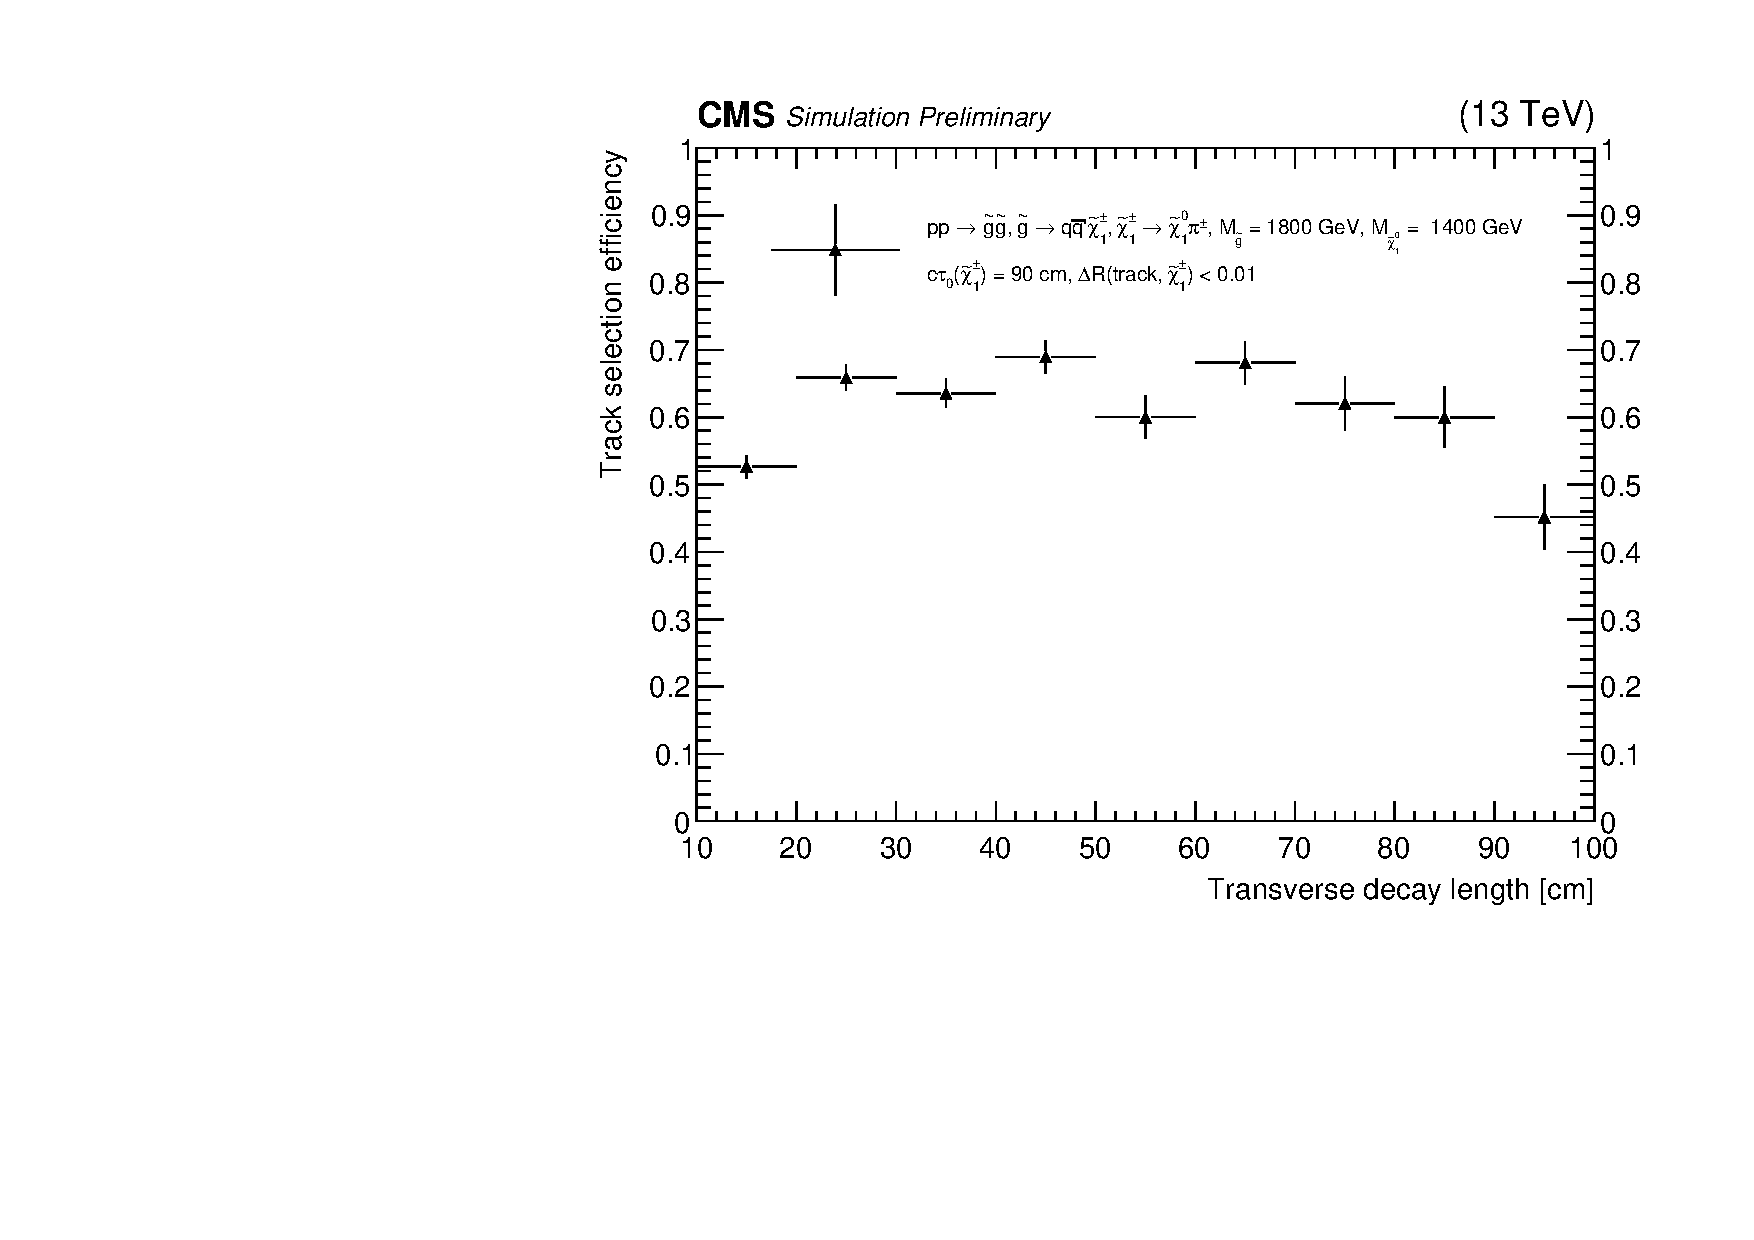
\includegraphics[width=0.85\textwidth]{figures/sigeff_bylength.pdf}
      \caption[Signal efficiency with respect to the short track selection.]
              {The signal efficiency with respect to the full short track selection after selecting events passing the baseline kinematic signal region selection.
                Additional material from \cite{MT2_2019}.}
      \label{fig:distrackssigeff}
    \end{figure}  

    The efficiency for signal tracks to pass this selection is high, 50--65\%, as shown in Figure~\ref{fig:distrackssigeff}.

    \subsubsection{Binning} \label{sec:distracksbinning}

    The background for shorter disappearing tracks is dominated by fakes, while the background for longer disappearing tracks is dominated by lost pions.
    Additionally, signals with different LLP lifetimes produce tracks of different lengths.
    Thus, binning the signal region by track length allows backgrounds of different origins to be segregated in different bins, and maximizes sensitivity to a variety of signal lifetimes.
    The disappearing track search adopts 3 categories of tracks length.
    \begin{itemize}
      \item Pixel-only (P) tracks have hits only inside the pixel tracker. Fakes dominate the background. In 2017 and 2018 data, these tracks are further subdivided into pixel tracks with hits in 3 distinct layers (P3) and pixel tracks with hits in 4 distinct layers (P4).
      \item Medium length (M) tracks have hits in fewer than 7 distinct layers, but have at least one hit outside the pixel detector. Lost mesons dominate the background.
      \item Relatively long (L) tracks have hits in 7 or more distinct layers, but still disappear, having missing expected hits in at least the two outermost layers of the tracker. Lost mesons dominate the background, and the better opportunity to measure the track allows for an especially tight selection, allowing for extremely strong background suppression.
    \end{itemize}
    Additionally, P and M tracks are divided into tracks with $15 < \pt < 50$~GeV (``lo'') and tracks with $\pt \geq 50$~GeV (``hi'').
    Most background falls into the low \pt bins, and signals generically populate the high \pt bins, making the high \pt bins the drivers of sensitivity to most signals.
    This division is not adopted for L tracks, as statistics are too low to allow further division of that population of tracks.

    Finally, events are binned based on the global event kinematics, using \njet and \Ht, again partly to segregate backgrounds produced by different signals and partly to enhance sensitivity to a variety of signal models.
    The \njet bins are $2 < \njet \leq 3$ (denoted by a trailing L, targeted at squark production), and $\njet > 4$ (H, targeted at gluino production).
    The \Ht bins are $250 < \Ht < 575$~GeV (denoted by a leading ``L''), $575 \leq \Ht < 1200$~GeV (``M''), and $\Ht \geq 1200$~GeV (``H'').
    For events with L length tracks, the L and M \Ht bins are merged into ``LM'' to preserve statistics.

    For example, the ``L HLM'' region is populated by events with L length tracks, with $\njet \geq 4$ and $\Ht \geq 1200$~GeV.
    The ``M LM lo'' region is populated by events with M length tracks of $15 < \pt < 50$~GeV, with $2 \njet \leq 3$ and $250 < \Ht < 575$~GeV.

    The STC control region binning mirrors the ST signal region, with each STC bin mapping to a corresponding ST bin.

    \subsubsection{Short Track Candidates and \fshort} \label{sec:fshort}

    The background estimation procedure makes use of the ratio of the counts of STs and STCs, called \fshort,
    \begin{equation}
      \fshort = \frac{N_{\mathrm{ST}}}{N_{\mathrm{STC}}}.
      \label{eqn:fshort}
    \end{equation}
    This ratio is measured in events with $60 < \mttwo < 100$~GeV, as these events are so background-dominated that even STs are assuredly background-dominated.
    A separate \fshort is measured for every bin, except that the measurement is inclusive in \Ht, exploiting an empirical invariance of \fshort with respect to \Ht to improve the statistical precision of the measurement.
    The ratio is then applied at high \mttwo to estimate the number of signal-like STs produced by background, $N_{\mathrm{ST}}^{\mathrm{B}}$, using the number of STC events observed in the corresponding control region, $N_{\mathrm{STC}}^{\mathrm{Obs}}$,
    \begin{equation}
      N_{\mathrm{ST}}^{\mathrm{B}} = \fshort N_{\mathrm{STC}}^{\mathrm{Obs}}.
      \label{eqn:fshortest}
    \end{equation}
    This estimate is correct up to statistical fluctuations, subject to the assumption that \fshort is invariant with respect to \mttwo, an assumption which is validated in data in the next subsection.
    Even without this explicit validation, there is no reason to expect that a ratio based on track-level observables, namely the impact parameter, \pt error, and isolation, ought to be sensitive to a global event kinematic variable like \mttwo.
    By tethering the background estimate to the observed count of STCs in data, the analysis is able to remain agnostic of the details of background disappearing track production.

    \subsubsection{Validation} \label{sec:distracksvalidation}

    \begin{figure}[h!]
      \centering
      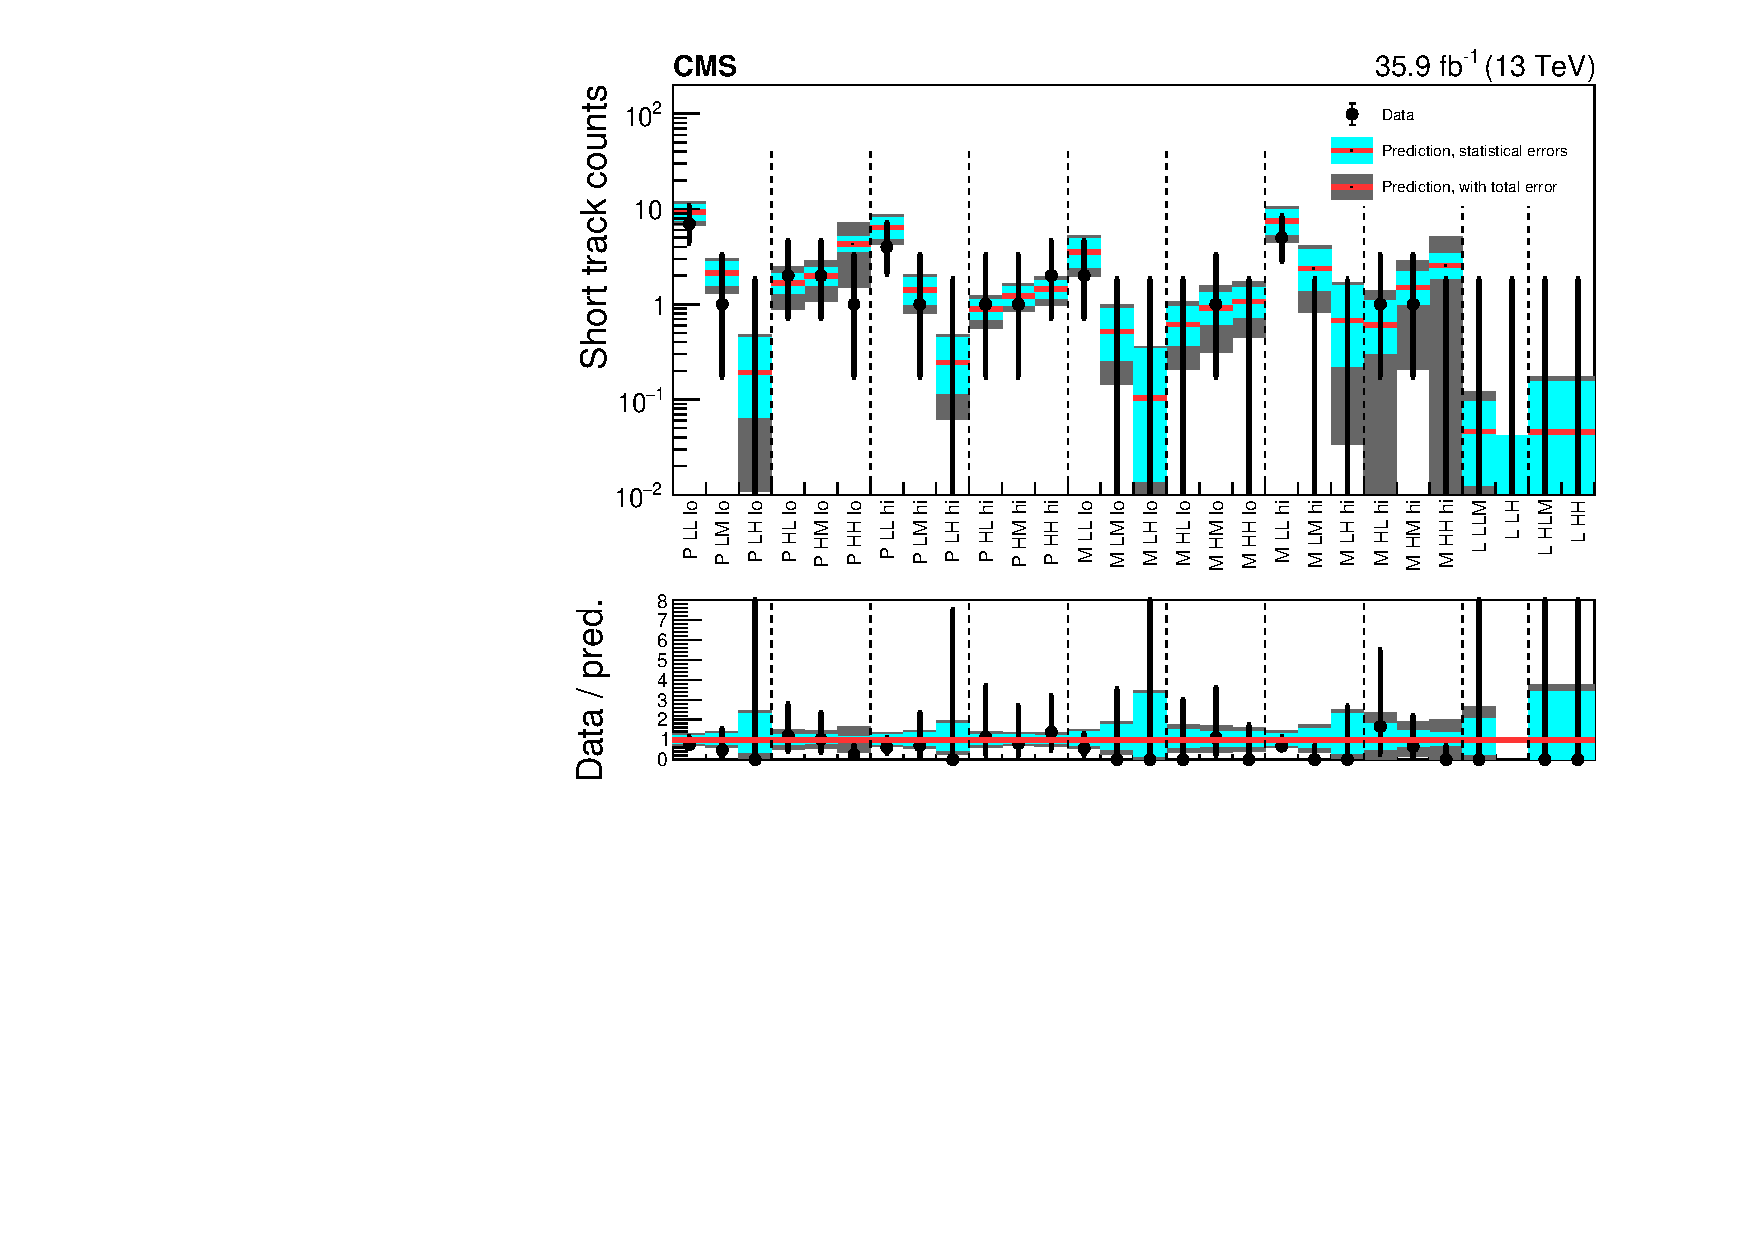
\includegraphics[width=0.85\textwidth]{figures/MT2_2019/Figure_004-a.pdf}
      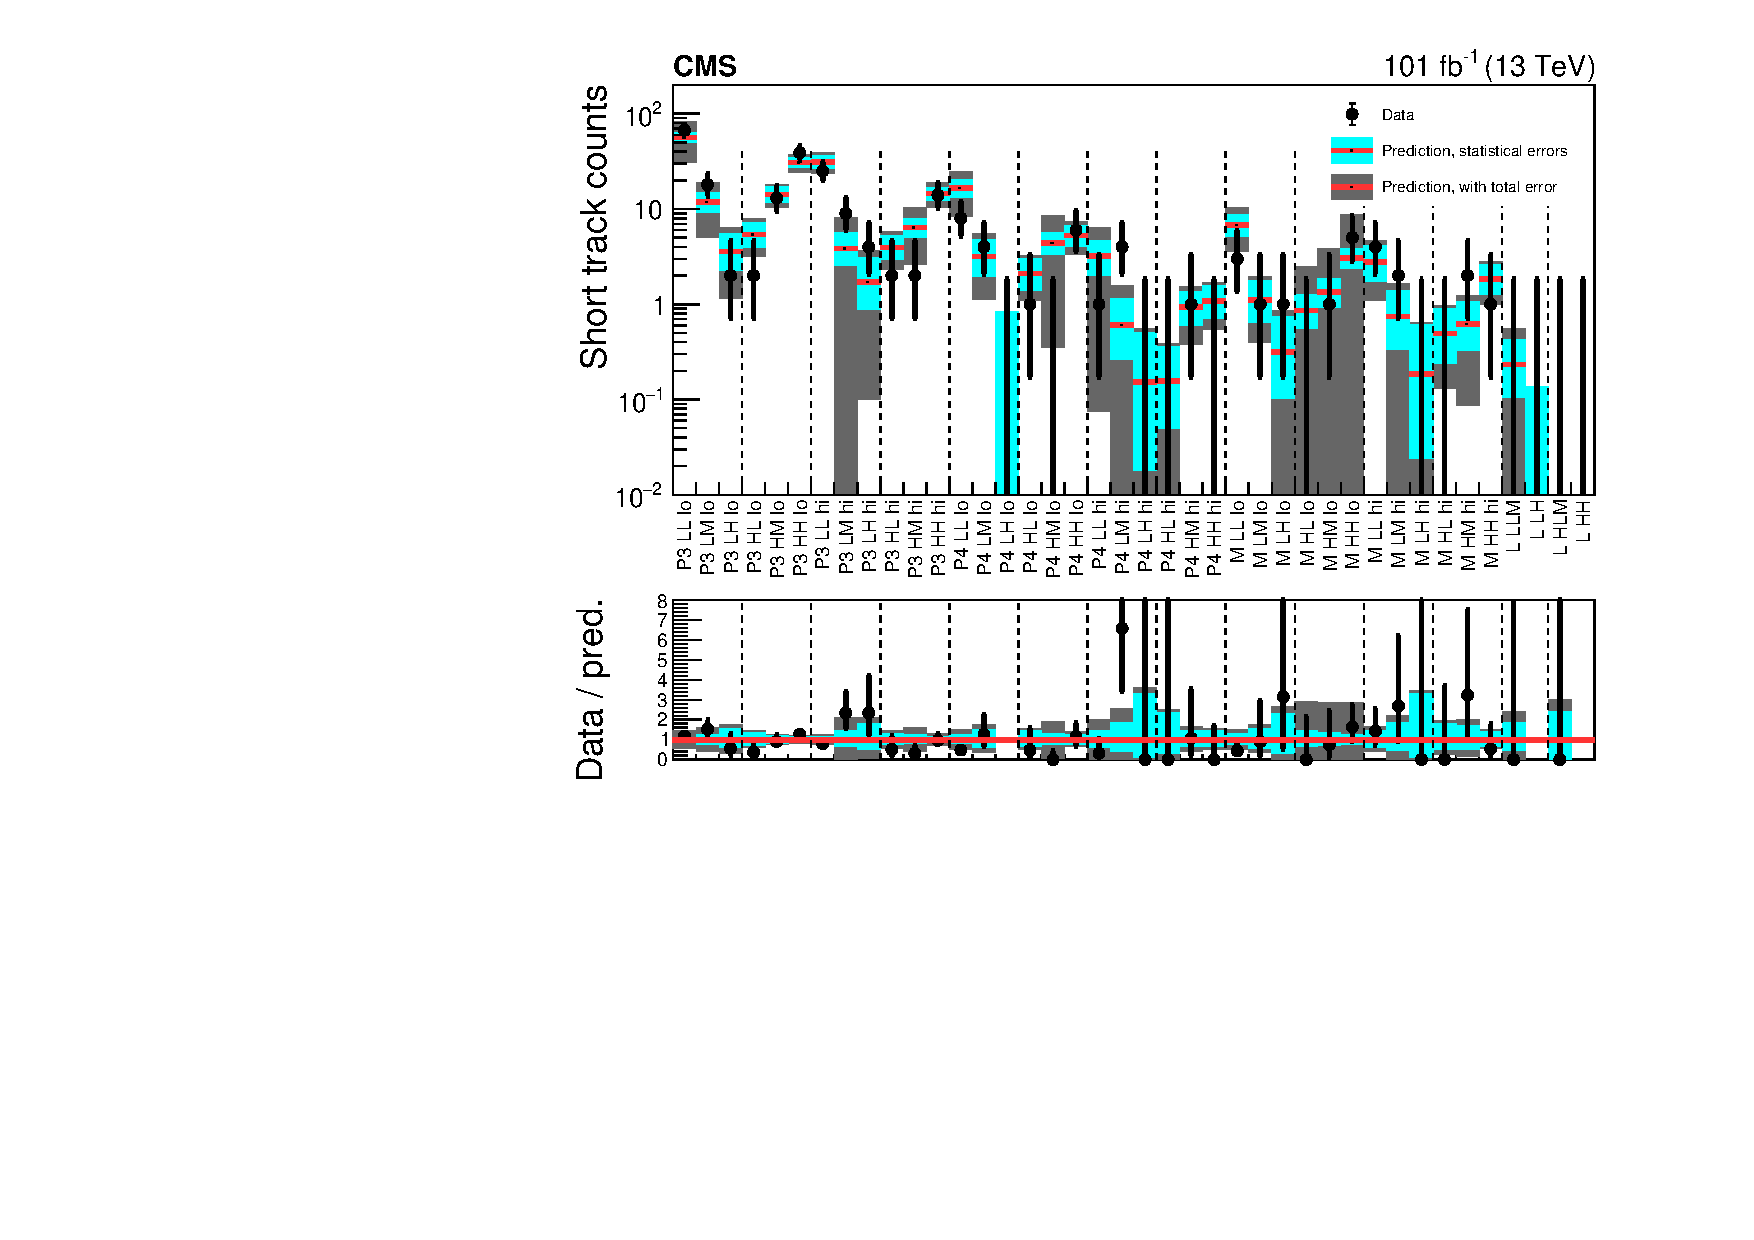
\includegraphics[width=0.85\textwidth]{figures/MT2_2019/Figure_004-b.pdf}
      \caption[Validation of the disappearing tracks background estimate in (upper) 2016 and (lower) 2017--2018 data.]
              {Validation of the disappearing tracks background estimate in (upper) 2016 and (lower) 2017--2018 data.
                There are no discrepancies inconsistent with statistical fluctuations.
                To be conservative, a systematic uncertainty (gray) is assessed region-by-region to account for any discrepancy greater than 1 statistical standard deviation (blue).
                Dotted vertical lines group bins that use the same measured value of \fshort, because they differ only in \Ht.
                Taken from \cite{MT2_2019}.}
      \label{fig:distracksval}
    \end{figure}  

    The \fshort-based estimate of background ST production relies on the invariance of \fshort with respect to \mttwo. 
    The \fshort ratio is measured at $60 < \mttwo < 100$~GeV, a background-dominated region, and applied in the $\mttwo > 200$~GeV signal region. 
    In Figure~\ref{fig:distracksval}, the invariance of \fshort with respect to \mttwo is validated in the intermediate region, $100 < \mttwo < 200$~GeV, in both 2016 and 2017--2018 data, by carrying out the background estimation procedure as used for the signal region in this \mttwo sideband.
    There are no discrepancies inconsistent with statistical fluctuations, so the estimate is considered validated.
    To be conservative, a systematic uncertainty is assessed bin-by-bin that is no less than the statistical uncertainty, to prevent any cases of accidental closure, and as large as is necessary to cover any observed discrepancy larger than 1 standard deviation of statistical uncertainty.

  \subsection{Systematics} \label{sec:distrackssysts}

  \begin{table}[htb!]
    \centering
    \topcaption[Table of uncertainties affecting the disappearing tracks background prediction.]{\label{tab:distracksyst}
      Summary of systematic uncertainties in the disappearing track background prediction, together with their typical size ranges across the search bins.
      The systematic uncertainties arising from the assumption of kinematic invariance of \fshort and from the validation of the background prediction are always taken
      to be at least as large as the statistical uncertainties on the measured values of  \fshort and on the background prediction in the validation region,
      respectively.
      Taken from \cite{MT2_2019}.
    }
    \begin{tabular}{ l  c }
      \hline
      Source & Range [\%] \\
      \hline
      Limited size of data control samples (high \mttwo STC counts) & 1--100\\
      Limited size of data \fshort measurement samples (low \mttwo disappearing track counts) & 5--45\\
      Kinematic invariance of \fshort & 10--80\\
      Validation of background prediction & 25--75\\
      \hline
    \end{tabular}
  \end{table}
  
  The uncertainties uniquely affecting the disappearing tracks the background prediction, in addition to those obtained from the validation region, are summarized in Table~\ref{tab:distracksyst} together with their typical size ranges across the search bins.

  The first two uncertainties are purely statistical and dominate the total uncertainty. 

  The kinematic invariance of \fshort is checked by varying the \Ht and \met definitions of the \fshort measurement region.
  Any uncertainty greater than 1 statistical standard deviation is covered by applying a systematic, just as for the validation region systematic.
  Although the relative uncertainties thus assessed can be large, this is an artifact of extremely low statistics.
  Discrepancies easily consistent within 2 statistical standard deviations can nonetheless lead to assessment of a large relative systematic uncertainty.
  Still, these uncertainties are applied to ensure that the disappearing tracks search is conservative.

  As for the classic search, the disappearing tracks signal simulation is subject to extra uncertainties, all of which are shared except the uncertainties assessed to cover the reconstruction of signal disappearing tracks, produced by decaying \chargino.
  There are three such uncertainties.

  First, fast simulation is used for signals simulated in 2017 and 2018 conditions. 
  The selection efficiency for signal tracks in fast simulation differs slightly from full simulation, and so a systematic is assessed to cover the difference.

  A 10\% uncertainty is assessed to cover any potential mismodeling of how efficiently the detector would reconstruct tracks from a long-lived \chargino.
  This is half the difference between unity and the observed efficiency in simulation, for \chargino decays in the regions of the detector that ought to be able to reconstruct the tracks successfully.

  Finally, an uncertainty of 1.5\% is assessed to cover observed differences between full simulation and fast simulation in how often a \chargino that reaches the muon chamber is falsely reconstructed as a muon, triggering the lepton veto.

  \subsection{Results} \label{sec:distracksresults}

  \begin{figure}[h!]
    \centering
    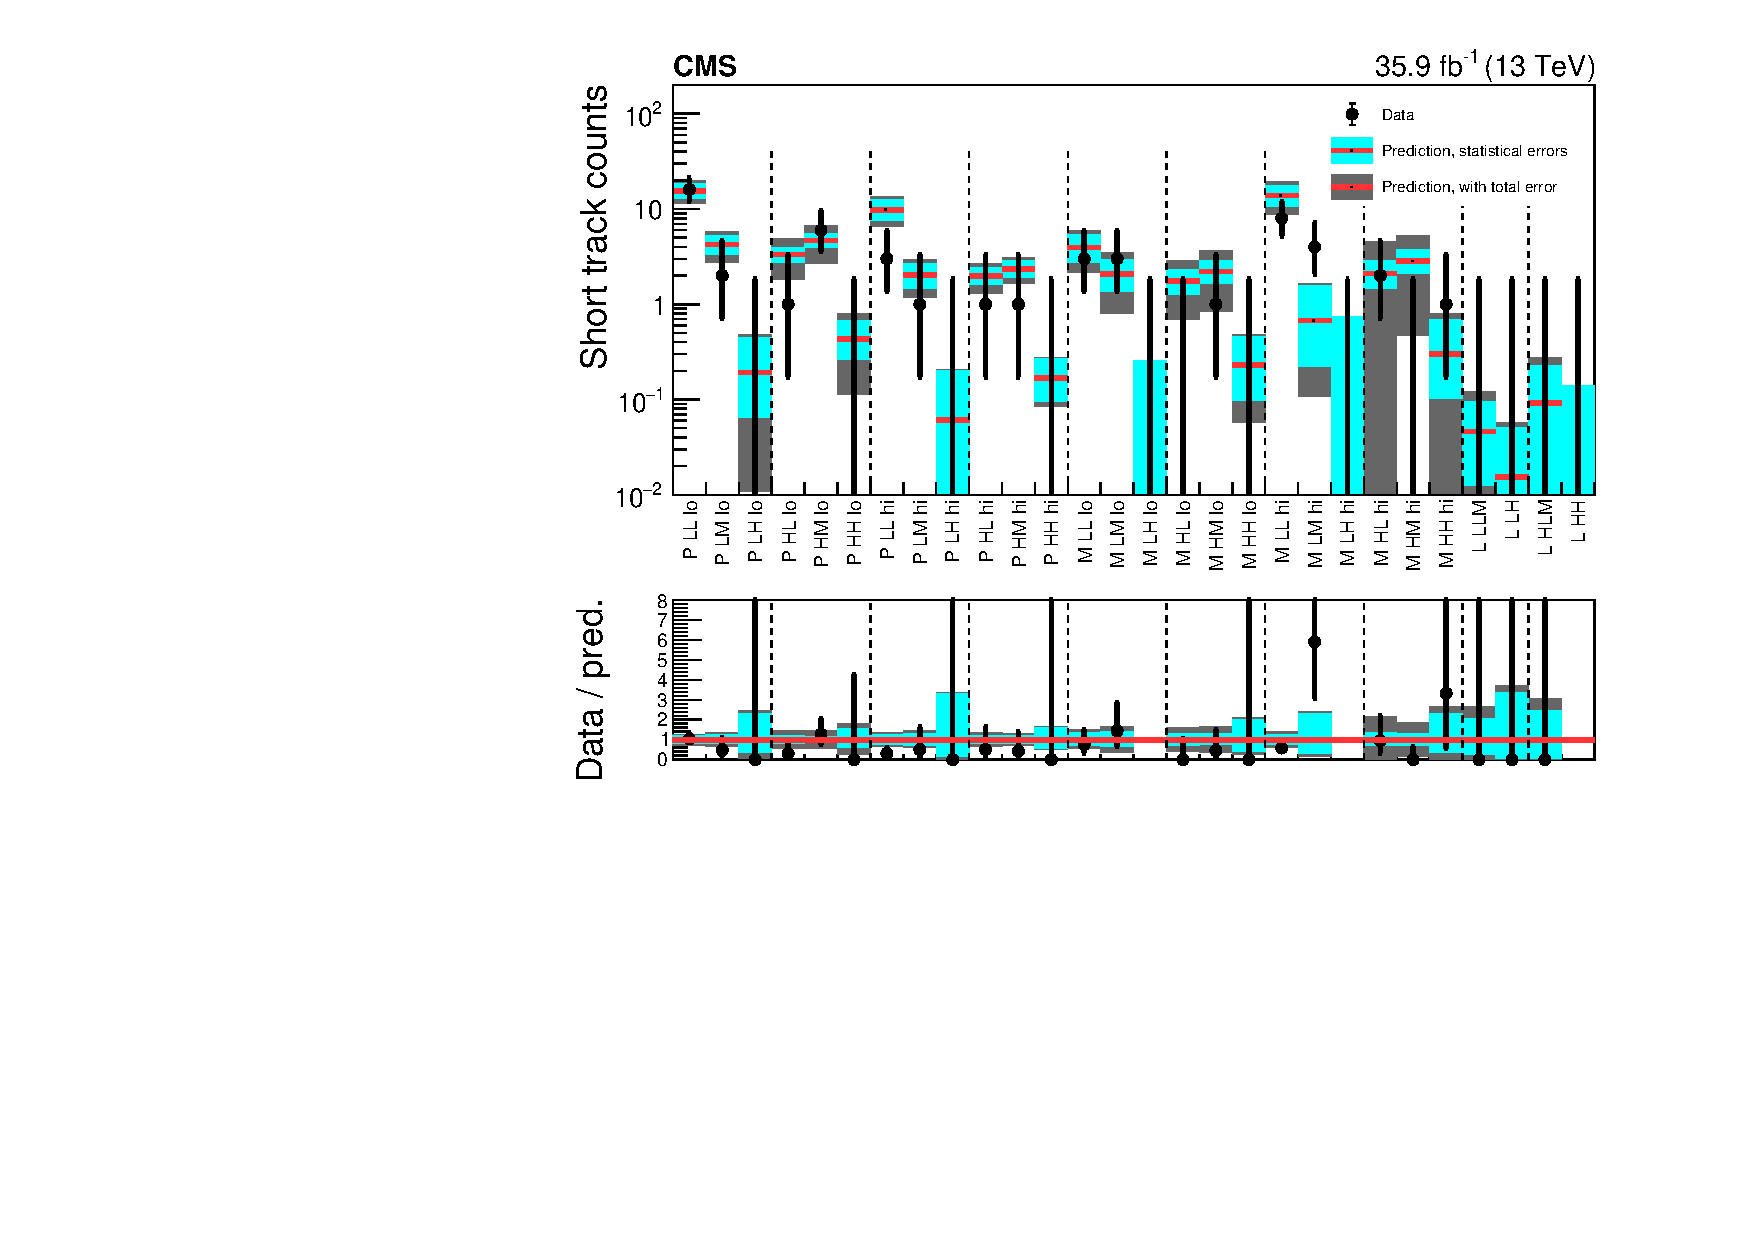
\includegraphics[width=0.85\textwidth]{figures/MT2_2019/Figure_006-a.pdf}
    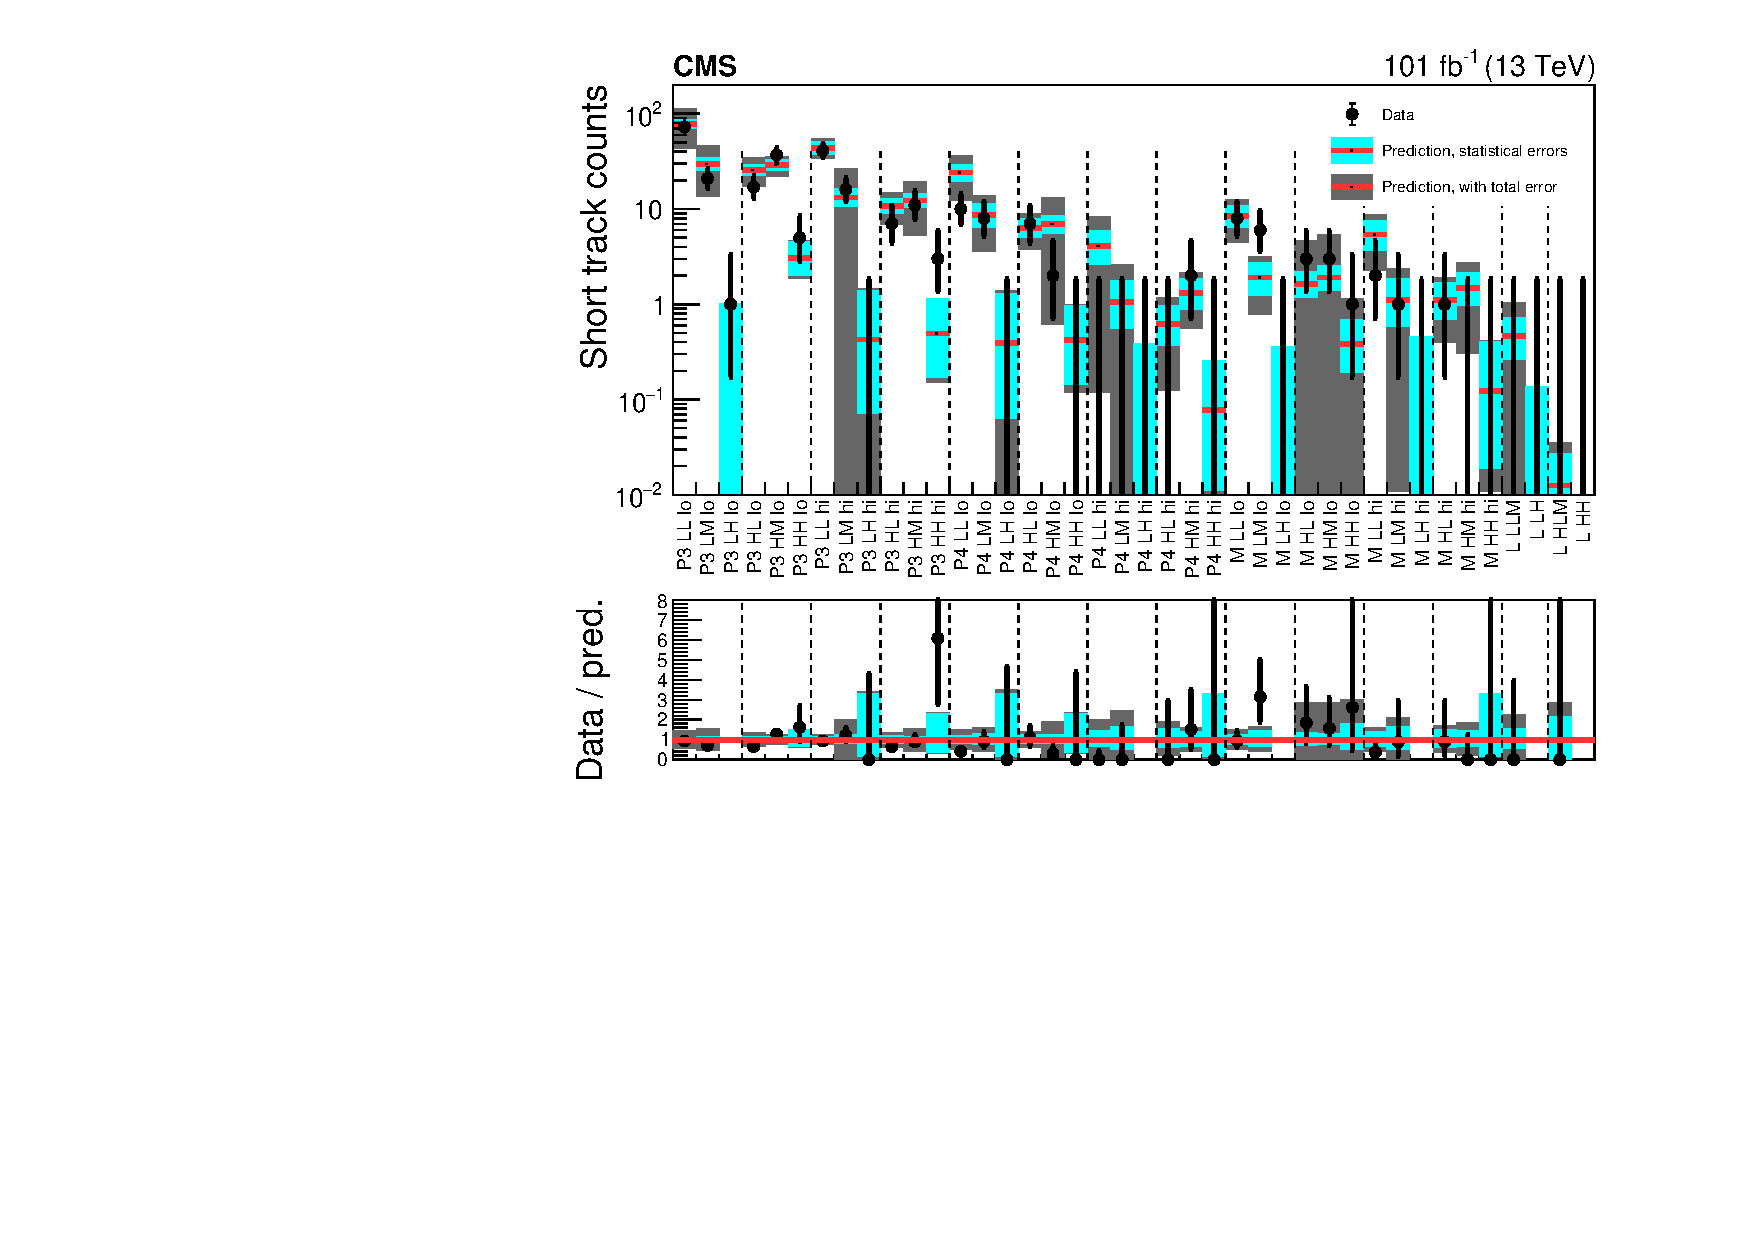
\includegraphics[width=0.85\textwidth]{figures/MT2_2019/Figure_006-b.pdf}
    \caption[Comparison of the predicted background and observed data events in the disappearing track search for (upper) 2016 and (lower) 2017--2018.]{Taken from \cite{MT2_2019}}
    \label{fig:distracksresults}
  \end{figure}  

  Figure~\ref{fig:distracksresults} shows the observed counts compared with the background estimate for both 2016 and 2017--2018 data.
  It is worth noting how small the expected background is, especially in the high \pt M and L bins, in which only a few events are observed across the entire 13 TeV dataset recorded from 2016 to 2018, at an event rate on the order of 1 GHz.
  The background-only hypothesis is consistent with the data, and so these results are interpreted as exclusion limits on the signal models shown in Figure~\ref{fig:charginodiags} with a variety of lifetimes.
  Since counts in the M and L bins are so small, signals populating the M and L bins need only to have a few expected events to be excluded at 95\% CL by these results.



    \subsubsection{Signal Contamination} \label{sec:distrackssigcontam}

    As with the contamination of lepton control regions in the classic search (Section~\ref{sec:MT2sigcontam}), the disappearing tracks search must adjust its expected signal counts for contamination of its control regions.
    In this case, there is some additional complexity because the signal can contaminate the background estimate by multiple routes.
    Any signal tracks in the \fshort measurement region at low \mttwo can bias the measurement of \fshort, and signal STCs in the high \mttwo STC control regions can bias the application of \fshort.
    We can separate these two factors to express the effect of contamination bias schematically as,
    \begin{equation}
      N_{\mathrm{ST}}^{\mathrm{Est}} + N_{\mathrm{Signal}}^{\mathrm{Bias}} = (\fshort+\Delta\fshort)(N_{\mathrm{STC}}+\Delta N_{\mathrm{STC}}) = \fshort N_{\mathrm{STC}}+\fshort\Delta N_{\mathrm{STC}} + \Delta\fshort N_{\mathrm{STC}} + \Delta\fshort\Delta N_{\mathrm{STC}}
      \label{eqn:fullsigcontam}
    \end{equation}
    The bias is not linear in the signal strength, due both to the manifestly nonlinear final term, $\Delta\fshort\Delta N_{\mathrm{STC}}$, and to the hidden nonlinearity in $\Delta\fshort$, 
    \begin{equation}
      \fshort + \Delta\fshort = \frac{N_{\mathrm{ST}}^{\mathrm{B}}+N_{\mathrm{ST}}^{\mathrm{S}}}{N_{\mathrm{STC}}^{\mathrm{B}}+N_{\mathrm{STC}}^{\mathrm{S}}}
    \end{equation}
    (Recall that these quantities are measured in the $60 < \mttwo < 100$~GeV sideband for the \fshort measurement.)
    
    If the overprediction of background due to contamination, $N_{\mathrm{Signal}}^{\mathrm{Bias}}$, is nonlinear, then the contamination factor $C$ is a function of the signal strength $\mu$, which means that the adjusted signal count must be recomputed for every trial signal strength during the statistical analysis,
    \begin{equation}
      N_{\mathrm{Signal}}^{\mathrm{Adjusted}} = \mu\left(N_{\mathrm{Signal}}^{\mathrm{Raw}}-N_{\mathrm{Signal}}^{\mathrm{Bias}}\right) = \mu \left(1-\frac{N_{\mathrm{Signal}}^{\mathrm{Bias}}}{N_{\mathrm{Signal}}^{\mathrm{Raw}}}\right)N_{\mathrm{Signal}}^{\mathrm{Raw}} = \mu C(\mu) N_{\mathrm{Signal}}^{\mathrm{Raw}}.
    \end{equation}
    This is computationally utterly infeasible.
    Fortunately, $N_{\mathrm{Signal}}^{\mathrm{Bias}}$ is {\it approximately} linear in $\mu$, and the approximation error is strictly conservative, so that adopting the approximation will never lead to a false discovery or false exclusion.
    
    First, one may approximate $\Delta \fshort$ thus,
    \begin{equation}
      \fshort + \Delta\fshort = \frac{N_{\mathrm{ST}}^{\mathrm{B}}+N_{\mathrm{ST}}^{\mathrm{S}}}{N_{\mathrm{STC}}^{\mathrm{B}}}.
    \end{equation}
    The term $N_{\mathrm{STC}}^{\mathrm{S}}$ is doubly small.
    First, signal is rare relative to background at low \mttwo, and second, only on the order of 1\% of signal tracks fall into the STC category, so that $N_{\mathrm{STC}}^{\mathrm{S}} \ll N_{\mathrm{STC}}^{\mathrm{B}}$ in the \fshort measurement region.
    This approximation linearizes $\Delta\fshort$, and strictly makes $\Delta\fshort$ larger by reducing the denominator, tending to overestimate the bias and, therefore, produce conservative signal counts.

    Next, adjusting the applied \fshort to $\fshort^{\prime}=\fshort-\Delta\fshort$, Equation~\ref{eqn:fullsigcontam} becomes
    \begin{equation}
      N_{\mathrm{ST}}^{\mathrm{Est}} + N_{\mathrm{Signal}}^{\mathrm{Bias}} = \fshort^{\prime}(N_{\mathrm{STC}}+\Delta N_{\mathrm{STC}}) = \fshort^{\prime}N_{\mathrm{STC}} + \fshort^{\prime}\Delta N_{\mathrm{STC}}
    \end{equation}
    The second component of $\fshort^{\prime}\Delta N_{\mathrm{STC}} = \fshort\Delta N_{\mathrm{STC}} - \Delta\fshort\Delta N_{\mathrm{STC}}$ is nonlinear in the signal strength, but is again doubly small, for the same reasons as the first neglected term.
    Neglecting it again produces a strictly larger estimate of the contamination, making the approximation conservative once again.

    Ultimately, then, there are two adjustments to the expected signal counts.
    First, the analysis subtracts the effect of signal contamination of low \mttwo STs, which bias the \fshort measurement.
    Then, the analysis subtracts the effect of signal contamination of high \mttwo STCs, which bias the application of \fshort.
    Both of these effects are small.
    Any terms that consider the combined effect of low \mttwo signal and signal STCs are dropped, as signal is rare in both cases, and so doubly rare in the combined case.
    This procedure outputs an adjustment to expected signal counts that is linear in the signal strength, and conservative, allowing for a straightforward and safe statistical interpretation.

  \subsection{Limits} \label{sec:distrackslimits}

  \begin{figure*}[htbp]
    \centering
    \includegraphics[width=0.48\textwidth]{figures/MT2_2019/Figure_017-a}
    \includegraphics[width=0.48\textwidth]{figures/MT2_2019/Figure_017-b}
    \includegraphics[width=0.48\textwidth]{figures/MT2_2019/Figure_017-c}
    \caption[Exclusion limits at 95\% \CL for gluino pair production, in the disappearing tracks search.]
            {Exclusion limits at 95\% \CL for direct gluino pair production where the gluinos decay to light-flavor quarks, with $c\tau_{0}(\chargino) =$ (upper left) 10\cm, (upper right) 50\cm, and (lower) 200\cm. Taken from \cite{MT2_2019}.}
    \label{fig:t1st_qqqq}
  \end{figure*}
  
  \begin{figure*}[htbp]
    \centering
    \includegraphics[width=0.48\textwidth]{figures/MT2_2019/Figure_018-a}
    \includegraphics[width=0.48\textwidth]{figures/MT2_2019/Figure_018-b}
    \includegraphics[width=0.48\textwidth]{figures/MT2_2019/Figure_018-c}
    \caption[Exclusion limits at 95\% \CL for light squark pair production, in the disappearing tracks search.]
      {Exclusion limits at 95\% \CL for light squark pair production with $c\tau_{0}(\chargino) =$ (upper left) 10\cm, (upper right) 50\cm, and (lower) 200\cm. 
        Taken from \cite{MT2_2019}.}
    \label{fig:t2st_qq}
  \end{figure*}
  
  \begin{figure*}[htbp]
    \centering
    \includegraphics[width=0.48\textwidth]{figures/MT2_2019/Figure_019-a}
    \includegraphics[width=0.48\textwidth]{figures/MT2_2019/Figure_019-b}
    \includegraphics[width=0.48\textwidth]{figures/MT2_2019/Figure_019-c}
    \caption[Exclusion limits at 95\% \CL for top squark pair production, in the disappearing tracks search.]
      {Exclusion limits at 95\% \CL for top squark pair production with $c\tau_{0}(\chargino) =$ (upper left) 10\cm (upper right) 50\cm, and (lower) 200\cm. Taken from \cite{MT2_2019}.}
    \label{fig:t2st_tt}
  \end{figure*}
  
  \begin{figure*}[htbp]
    \centering
    \includegraphics[width=0.48\textwidth]{figures/MT2_2019/Figure_020-a}\\
    \includegraphics[width=0.48\textwidth]{figures/MT2_2019/Figure_020-b}
    \includegraphics[width=0.48\textwidth]{figures/MT2_2019/Figure_020-c}
    \caption[Exclusion limits at 95\% \CL on the \lsp mass as a function of \chargino proper decay length for gluino pair production and decay to light quarks, and light squark pair production, in the disappearing tracks search.]
      {Exclusion limits at 95\% \CL on the \lsp mass, with $m_{\chargino}=m_{\lsp}+\mathcal{O}(100\MeV)$, as a function of the \chargino proper decay length,
      for (upper) direct gluino and (lower) direct light-flavor squark pair production, for representative gluino and squark masses. Taken from \cite{MT2_2019}.}
    \label{fig:limits1fixedmass}
  \end{figure*}
  
  \begin{figure}[htb!]
    \centering
    \includegraphics[width=0.48\textwidth]{figures/MT2_2019/Figure_021}
    \caption[Exclusion limits at 95\% \CL on the \lsp mass as a function of \chargino proper decay length for top squark pair production, in the disappearing tracks search.]
      {Exclusion limits at  95\% \CL on the \lsp mass, with $m_{\chargino}=m_{\lsp}+\mathcal{O}(100\MeV)$, as a function of the \chargino proper decay length,
      for direct top squark pair production, as obtained for a representative top squark mass. Taken from \cite{MT2_2019}.}
    \label{fig:limits1fixedmass_stop}
  \end{figure}
  
  \begin{figure*}[htbp]
    \centering
    \includegraphics[width=0.48\textwidth]{figures/MT2_2019/Figure_022-a}\\
    \includegraphics[width=0.48\textwidth]{figures/MT2_2019/Figure_022-b}
    \includegraphics[width=0.48\textwidth]{figures/MT2_2019/Figure_022-c}
    \caption[Exclusion limits at 95\% \CL on gluino, light squark, and top squark pair production cross sections as a function of \chargino proper decay length, in the disappearing tracks search.]
      {Exclusion limits at 95\% \CL on $\sigma/\sigma_{\mathrm{theory}}$ as a function of the \chargino decay length, for
      (upper) gluino pair production where the gluinos decay to light-flavor quarks, (lower left) light-flavor squark pair production,
      and (lower right) top squark pair production, as obtained from the search for disappearing tracks. Taken from \cite{MT2_2019}.}
    \label{fig:limits2fixedmasses}
  \end{figure*}
  
  The statistical procedure for extracting limits in the disappearing tracks search is exactly identical to that used in the classic search, described in Section~\ref{sec:MT2limits}, with the addition of the LLP lifetime as a parameter of interest.
  Figures~\ref{fig:t1st_qqqq}-\ref{fig:t2st_tt} show limits in the mass plane for gluinos decaying to light squarks, bottom squarks, and top squarks, respectively, with the \chargino $c\tau$ set to 10~cm~(upper left), 50~cm~(upper right), and 200~cm~(bottom).
  These limits can be compared directly to those obtained by the classic search, shown respectively in Figures~\ref{fig:t5x} (upper), \ref{fig:t2x} (upper left), and \ref{fig:stop_other} (upper right).
  In each case, the limits improve by hundreds of GeV along each axis, due entirely to the strong background suppression of the ST requirement.
  
  An interesting feature of these exclusion curves is evident when comparing longer to shorter \chargino lifetimes.
  For $c\tau = 200$~cm, the limit curve abruptly turns inward at the bottom right of each plot, where the gluino or squark is much more massive than \chargino and \lsp.
  At $c\tau = 50$~cm, this feature is reduced in prominence, and it is inverted when $c\tau = 10$~cm.
  This is caused by the large Lorentz boost and correspondingly extended lab frame lifetime of \chargino in these mass scenarios.
  At longer lifetimes, \chargino often lives long enough to escape the tracker, or at least make it near enough to the edge not to leave a disappearing track, defined as a track with at least two tracker layers missing expected hits.
  With no disappearing track, the event fails the ST selection, so the signal efficiency for long \chargino lifetime is reduced in the large mass splitting scenario, and limits are weakened.
  In contrast, shorter lifetimes benefit from the boost, as tracks more often extend into the more sensitive M and L bins.
  Masses of \chargino below 91.9~GeV are excluded by searches at CERN's Large Electron Positron collider \cite{lep_chargino}, while previously occupied the LHC tunnel, mitigating the impact of this effect.

  Figures~\ref{fig:limits1fixedmass} and ~\ref{fig:limits1fixedmass_stop} show limits at 95\% CL on the \lsp mass as a function of the lifetime of \chargino, at representative fixed masses of the considered gluino or squark, with the 68\% and 95\% uncertainty bands shown in green and yellow, respectively.
  Figure~\ref{fig:limits1fixedmass} (upper) considers gluino pair production at gluino mass 1900~GeV.
  Figure~\ref{fig:limits1fixedmass} (lower left) considers light squark pair production in the case of a single light squark of mass 900~GeV.
  Figure~\ref{fig:limits1fixedmass} (lower right) considers light squark pair production in the case of eight degenerate light squarks of mass 1500~GeV.
  Figure~\ref{fig:limits1fixedmass_stop} considers top squark pair production and at top squark mass 1000~GeV.

  There is a discontinuity at low \chargino lifetime in the exclusion curves of all four of these figures.
  At this discontinuity, the limits obtained for the classic search, applicable to any \chargino of lifetime short enough not to reach the calorimeters, become superior to those obtained by the disappearing track search.
  At these very short lifetimes, many of the charginos decay before reaching the tracker or soon after, and so do not produce tracks.
  As the disappearing track search only selects events with a disappearing track, it suffers from large selection inefficiencies at these very short lifetimes.
  The classic search does not require a track, and so avoids this selection inefficiency, as the cost of a larger background.
  For short enough \chargino lifetimes, to the left of the discontinuity in each figure, this tradeoff becomes advantageous as measured by the expected sensitivity.

  When the exclusion curves approach the kinematic limit, at which the mass of the decaying particle and the mass of the \chargino are nearly equal, the errors tend to become greatly compressed.

  Finally, Figure~\ref{fig:limits2fixedmasses} show the exclusion limits at 95\% CL on the production cross section of gluinos and squarks as a function of \chargino lifetime for fixed gluino or squark mass and \lsp mass, for gluinos of mass 1600~GeV decaying to light quarks and \lsp of mass 1575~GeV (upper), light squarks of mass 2000~GeV and \lsp mass 1000~GeV (lower left), and top squarks of mass 1100~GeV and \lsp mass 1000~GeV (lower right).
  The limits are strongest for intermediate \chargino lifetimes for which the fraction of \chargino decays producing disappearing tracks tens of centimeters long is maximized.
  Sensitivity is lesser for longer and shorter lifetimes due to reduced efficiency to produce disappearing tracks, and consequently reduced signal selection efficiency.

  All of these limits are the strongest produced to date by any analysis, and constitute stringent constraints on the entire class of signal models discussed in Section~\ref{sec:distrackssig}.

  \subsection{Future} \label{sec:distracksfuture}
  
  The subject of LLPs in supersymmetric extensions of the Standard Model, and the potential sensitivity gains that LLPs can provide for new physics searches in general, will continue to inspire interest for the foreseeable future of the LHC's physics program.
  The \mttwo disappearing track extension is no exception.
  Furthermore, unlike the classic search, which has non-negligible backgrounds that will grow larger with increased integrated luminosity luminosity, the most sensitive bins of the disappearing tracks search are effectively entirely background-depleted.
  In fact, while the background should not meaningfully increase in the foreseeable future, the statistical precision of the background estimate {\it will} improve with the addition of more data.
  As a result, the sensitivity of the disappearing track search projects to improve roughly linearly with increasing integrated luminosity rather than as its square root.
  With continuing interest and better scaling of the sensitivity, this search is a potentially worthwhile candidate for continued updates as the CMS dataset expands.

  Additionally, the disappearing tracks search in its current form targets only tracks that disappear inside the silicon tracker, and does not consider the case of tracks disappearing inside the muon system, as mentioned in Section~\ref{sec:muon}.
  Indeed, it explicitly vetoes tracks potentially associated with hits in the muon system.
  However, sufficiently long-lived charginos would leave hits in the muon system, and so there exists a possibility to extend the lifetime sensitivity range of the disappearing tracks search by expanding the definition to include disappearing tracks in the muon system, or even non-disappearing tracks in the muon system that appear to be produced by a particle too heavy to be consistent with a muon.

  In any case, the disappearing tracks signature certainly has not been fully exploited, and will remain an interesting search strategy in future LHC datasets.


